\documentclass[11pt,a4paper]{article}

\usepackage[utf8]{inputenc}
\usepackage[T1]{fontenc}
\usepackage{lmodern}
\usepackage[a4paper,top=2.3cm,bottom=2.3cm,left=2.4cm,right=2.4cm]{geometry}
\usepackage{amsmath,amssymb,amsfonts,bm}
\usepackage{booktabs,array,tabularx,multirow}
\usepackage{graphicx}
\usepackage{xcolor}
\usepackage{siunitx}
\PassOptionsToPackage{hyphens,obeyspaces,spaces}{url}
\usepackage[backend=biber,style=ieee,sorting=none]{biblatex}
\addbibresource{references.bib}
\renewcommand*{\bibfont}{\small}
\setlength{\bibitemsep}{2pt}
\usepackage{microtype}
\usepackage[colorlinks=true,linkcolor=blue!55!black,citecolor=blue!55!black,urlcolor=blue!55!black]{hyperref}
\usepackage[capitalise,noabbrev]{cleveref}
\usepackage{enumitem}
\usepackage{titlesec}
\usepackage{placeins}
\usepackage{tikz}
\usetikzlibrary{arrows.meta,positioning,calc,patterns}

\DeclareSIUnit{\mbps}{Mbps}
\DeclareSIUnit{\kbps}{kbps}
\DeclareSIUnit{\pkt}{pkts}
\DeclareSIUnit{\tick}{ticks}
\DeclareSIUnit{\pp}{pp}
\DeclareSIUnit{\byte}{B}
\sisetup{
  group-separator={,},
  group-minimum-digits=4,
  group-digits=integer,
  retain-explicit-plus=true,
  mode=match,
  propagate-math-font=true,
  reset-math-version=false,
  reset-text-family=false,
  reset-text-series=false,
  reset-text-shape=false,
  text-family-to-math=true,
  text-series-to-math=true,
  per-mode=symbol
}

% Semantic notation macros (eliminating symbol overloading and inline-math clutter)
\newcommand{\Namr}{\ensuremath{N_{\mathrm{AMR}}}}
\newcommand{\ltel}{\ensuremath{\lambda_{\mathrm{tel}}}}
\newcommand{\Rphy}{\ensuremath{R_{\mathrm{PHY}}}}
\newcommand{\Tsuper}{\ensuremath{T_{\mathrm{super}}}}
\newcommand{\MissA}{\ensuremath{\operatorname{Miss}_A}}
\newcommand{\MissB}{\ensuremath{\operatorname{Miss}_B}}
\newcommand{\ploss}{\ensuremath{p_{\mathrm{loss}}}}
\newcommand{\Wone}{\ensuremath{\mathcal{W}_1}}
\newcommand{\rdist}{\ensuremath{r_{\mathrm{dist}}}}
\newcommand{\GainP}{\ensuremath{\Delta_{\mathrm{P}}}}
\newcommand{\GainS}{\ensuremath{\Delta_{\mathrm{S}}}}
\newcommand{\GainW}{\ensuremath{\Delta_{\mathrm{W}}}}
\newcommand{\GainPbar}{\ensuremath{\bar{\Delta}_{\mathrm{P}}}}
\newcommand{\GainSbar}{\ensuremath{\bar{\Delta}_{\mathrm{S}}}}
\newcommand{\GainWbar}{\ensuremath{\bar{\Delta}_{\mathrm{W}}}}
\newcommand{\GainPpair}{\ensuremath{\Delta_{\mathrm{P}}^{(1\to 3)}}}
\newcommand{\GainWpair}{\ensuremath{\Delta_{\mathrm{W}}^{(1\to 2)}}}

\setlist{nosep}
\emergencystretch=1.5em
\Urlmuskip=0mu plus 2mu\relax
\newcolumntype{Y}{>{\raggedright\arraybackslash}X}
\newcolumntype{P}[1]{>{\raggedright\arraybackslash}p{#1}}
\newcolumntype{R}[1]{>{\raggedleft\arraybackslash}p{#1}}
\newcolumntype{C}[1]{>{\centering\arraybackslash}p{#1}}

\definecolor{cWlan}{HTML}{D55E00}
\definecolor{cSw}{HTML}{0072B2}
\definecolor{cWire}{HTML}{7F7F7F}
\definecolor{cTeal}{HTML}{009E73}

\titleformat{\section}{\large\bfseries}{\thesection}{0.8em}{}
\titleformat{\subsection}{\normalsize\bfseries}{\thesubsection}{0.8em}{}
\titleformat{\subsubsection}{\normalsize\itshape}{\thesubsubsection}{0.8em}{}
\titlespacing*{\section}{0pt}{1.8ex plus 0.4ex minus 0.2ex}{0.8ex plus 0.2ex}
\titlespacing*{\subsection}{0pt}{1.4ex plus 0.3ex minus 0.2ex}{0.5ex plus 0.1ex}
\titlespacing*{\subsubsection}{0pt}{1.1ex plus 0.2ex minus 0.1ex}{0.4ex plus 0.1ex}
\titlespacing*{\paragraph}{0pt}{0.9ex plus 0.2ex minus 0.1ex}{0.7em}

\setlength{\floatsep}{8pt plus 2pt minus 2pt}
\setlength{\textfloatsep}{10pt plus 2pt minus 3pt}
\setlength{\intextsep}{8pt plus 2pt minus 2pt}
\setlength{\abovecaptionskip}{4pt}
\setlength{\belowcaptionskip}{4pt}

\title{\textbf{Bottleneck Migration in Hybrid Wired and Wireless Industrial Networks: Validation}}

\author{
  \textbf{Breno da Silva Pereira} \qquad\qquad \textbf{Gabriel S. Stuart} \\[1.2ex]
  \textit{Advisor:} Prof.\ Dr.\ Ant\^{o}nio Augusto Medeiros Fr\"{o}hlich \\[1.2ex]
  Department of Informatics and Statistics (INE) \\
  Universidade Federal de Santa Catarina (UFSC) \\
  Florian\'{o}polis, SC, Brazil
}

\date{November 2026}

\begin{document}

\maketitle

\begin{abstract}
Modern matrix-manufacturing cells coordinate Autonomous Mobile Robots (AMRs) and fixed production stations through discrete-event digital twins whose end-to-end timeliness depends simultaneously on a wireless shop-floor link and a wired factory backbone. Because industrial networks are frequently upgraded incrementally, improving one communication domain in isolation can leave end-to-end deadlines dominated, or even degraded, by queueing and scheduling waits in the companion domain. Using OMNeT++/INET discrete-event simulation across a full 80-point factorial grid of fleet sizes, wireless physical bitrates, and background telemetry loads (\num{6947} runs), this study evaluates six hybrid architectures crossing three Ethernet switch disciplines (best-effort FIFO, IEEE~802.1Q strict priority, and a static IEEE~802.1Qbv time-aware shaper schedule) with two IEEE~802.11g wireless access mechanisms (contention-based CSMA/CA and fixed single-slot TDMA). Results show that wired strict priority eliminates backbone congestion for critical control traffic, whereas the configured static time-aware gate windows throttle heavy background telemetry. On the wireless link, TDMA eliminates access-point buffer drops and runaway contention tails in dense low-rate fleets, yet degrades uplink timeliness---and interacts negatively with a congested FIFO switch---when its fixed cycle exceeds the control deadline or when downlink slots are tightly provisioned. Under simultaneous wired and wireless saturation, eliminating critical physical loss alongside bounded delivered-packet staleness requires deterministic isolation in both domains, though sub-\qty{50}{\milli\second} state timeliness on the \qty{10}{\milli\second} tick grid at high density additionally requires \qty{54}{\mbps} PHY or multi-slot access. Three targeted verification pilots confirm that expanding and sub-blocking downlink TDMA slots lowers tick-grid command misses, port-specific switch gate rebalancing eliminates \qty{45.0}{\mbps} telemetry losses and leaves \qty{0.13}{\percent} at \qty{60.0}{\mbps} while still throttling above \qty{67.20}{\mbps}, and enlarging the 802.1Q low-priority queue eliminates near-saturation burst drops (\qty{0.47}{\percent} $\to$ \qty{0.00}{\percent} at \qty{85.0}{\mbps}) while deep-saturation overflow remains governed by priority preemption (\qty{38.93}{\percent} at \qty{149.3}{\mbps}). Finally, densifying the sampled grid across wired saturation transitions cuts Leave-One-Out Wasserstein interpolation error by \qtyrange{70.0}{71.1}{\percent} on shared-trunk classes.
\end{abstract}

\noindent\textbf{Keywords:} Time-Sensitive Networking, IEEE~802.1Qbv, IEEE~802.1Q, Scheduled Wireless Access, hybrid industrial networks, discrete-event simulation, OMNeT++/INET, digital twin, autonomous mobile robots.

% =============================================================================
\section{Introduction}
\label{sec:intro}

Whereas IEEE~1516.1-2010~\cite{ieee1516} defines the conservative \emph{Next Message Request} (NMR) time-advance service, the \textit{Matrix Factory Twin} implements a project-specific fixed-tick Next Event Request (NER) interface advancing the digital-twin clock in discrete ticks of period $T$ after resolving all events with earlier timestamps. Unlike continuous-time packet sinks, an NER consumer inspects network messages only at scheduled tick boundaries: control loops either discard late delivered commands exceeding a project-defined continuous Watchdog Time-To-Live ($a > g + D_c$, Watchdog KILL, making continuous $\MissA$ the Watchdog-enforced command unavailability metric, while $\MissB$ measures uniform NER tick-grid arrival timeliness without an intervening continuous watchdog)~\cite{pazzaglia2019dmac} or hold the previous state across missed NER ticks via Zero-Order Hold (ZOH), accumulating Age of Information and tick staleness~\cite{kaul2012real}. End-to-end timeliness across the factory floor depends simultaneously on the wireless link connecting mobile robots to the Access Point (AP) and the wired Ethernet backbone connecting fixed stations, the AP, and the central Fleet Management System (FMS).

Recent Wireless Time-Sensitive Networking (W-TSN) architectures extend deterministic scheduling from wired IEEE~802.1Q/802.1Qbv backbones to wireless access links~\cite{zanbouri2025survey, cavalcanti2019extending, seijo2022sharp}. In practice, however, industrial deployments often upgrade one domain at a time, retrofitting an IEEE~802.1Q or 802.1Qbv switch behind an existing IEEE~802.11 AP, or deploying scheduled TDMA wireless access over a best-effort switch. Evaluating this fixed-schedule hybrid network architecture across its full factorial parameter space, we first resolve three operational research questions and additionally test a naive additive domain-share baseline (\Cref{sec:rq2}) to separate regimes where linear drop and delay attribution holds from regimes where deterministic scheduling wait in the upgraded domain sums with queueing delay in the companion domain across a step deadline threshold.

We structure the investigation around three operational research questions:
\begin{enumerate}[label=\textbf{RQ-(\roman*)}, leftmargin=3.8em]
    \item \textbf{Isolated Domain Upgrades:} Under which background telemetry load ($\ltel$) and fleet size ($\Namr$) regimes does an isolated upgrade in either the wired Ethernet backbone or the wireless access link reduce application deadline misses?
    \item \textbf{Cross-Domain Masking and Negative Interaction:} When does congestion or structural scheduling wait in the companion domain mask or reverse the benefit of a local domain upgrade, and how do per-packet delay and drop shares explain this interaction?
    \item \textbf{Dual-Domain Determinism:} Which combinations of Ethernet load, fleet density, and physical data rate require deterministic mechanisms in both domains simultaneously to eliminate critical physical loss, bound observed delivered-packet staleness, and satisfy the distribution-free per-seed operating-envelope criterion?
\end{enumerate}

The remainder of this report defines the hybrid topology, literature-informed traffic inputs, packet-level timing semantics, and dataset structure in \Cref{sec:methodology}; derives analytical Ethernet, gate-window, wireless-airtime, and queueing limits in \Cref{sec:analytical}; synthesizes quantitative answers to RQ-(i) through RQ-(iii) (\Cref{tab:rq_summary}) in \Cref{sec:results}; examines contention collapse, multi-rate tick sensitivity, lookup interpolation error, and co-design schedule sensitivity in \Cref{sec:supporting}; discusses architectural implications and threats to validity in \Cref{sec:discussion}; synthesizes conclusions, future work, and artifact availability in \Cref{sec:conclusion}; and documents runtime-optimization equivalence and dataset traceability in \Cref{app:speedup,app:traceability}.

% =============================================================================
\section{Background and Related Work}
\label{sec:related_work}

\paragraph{Hybrid Wired and Wireless TSN Integration.}
Standard Ethernet TSN guarantees bounded latency on wired trunks through IEEE~802.1Q-2022 strict priority queuing (Clause~8.6.8.1) and scheduled traffic (Clause~8.6.8.4)~\cite{ieee8021q}, originally amended by IEEE~802.1Qbv~\cite{ieee8021qbv}. Extending these guarantees across wireless links is a central challenge in industrial automation~\cite{zanbouri2025survey}. Cavalcanti et al.~\cite{cavalcanti2019extending} analyze the architectural requirements and timing capabilities needed to extend TSN features over IEEE~802.11 WLANs, while Seijo et al.~\cite{seijo2022sharp} analytically model how misaligned wired GCL and wireless TDMA windows inject queuing jitter in their three-hop SHARP hybrid wired and wireless TSN architecture and experimentally evaluate congestion when wired scheduling is disabled. Whereas existing hardware testbeds and analytical evaluations focus on small-scale factory cells, including the three-hop SHARP testbed~\cite{seijo2022sharp}, small multi-node DDS/OPC~UA benchmarks~\cite{calvo2013dds, maia2020opcua}, and low-density AGV cells~\cite{11511549}, our factorial campaign characterizes how wired and wireless scheduling interact up to $\Namr=80$ AMRs and \qty{149.3}{\mbps} backbone loads.

\paragraph{IEEE 802.11 DCF Contention, Industrial WLANs, and Physical Capture.}
Under the IEEE~802.11 Distributed Coordination Function (DCF / CSMA/CA)~\cite{ieee80211}, collision probability and backoff delay grow non-linearly with the number of contending stations, as established by Bianchi's Markov chain analysis~\cite{bianchi2000performance} and industrial WLAN response-time studies by Cena et al.~\cite{cena2007evaluation}. In asymmetric star topologies where an AP dispatches downlink commands while dozens of stations contend on the uplink, the AP shares the same contention access opportunity as a single station, creating severe downlink queuing bottlenecks. Furthermore, when multiple uplink frames collide at the AP receiver, physical-layer capture allows a higher-power frame from a nearby station to survive Signal-to-Noise-plus-Interference Ratio (SNIR) decoding while distant stations suffer repeated retry-limit drops~\cite{lee2007experimental}. Our supporting diagnostics examine how these two mechanisms interact in dense AMR fleets.

\paragraph{Industrial Workloads and Digital-Twin Consumption Semantics.}
Modern matrix manufacturing multiplexes heterogeneous traffic classes: VDA~5050 fleet orders and state telemetry~\cite{vda5050, 11511549}, OMG Data Distribution Service (DDS) real-time inter-station coordination over RTPS/UDP~\cite{omgdds, omgrtps, calvo2013dds}, and OPC~UA / MQTT background machine telemetry~\cite{opcua, mqtt5, profanter2019opcua, maia2020opcua}. Empirical ICS traffic characterizations such as Brenner et al.~\cite{brenner2024ics} highlight mixed operational protocol payloads on factory links, motivating our stress-testing of background \qty{1400}{\byte} UDP bursts alongside critical control traffic. When feeding an HLA time-stepped or Next Message Request digital twin~\cite{ieee1516}, latency distributions cannot be judged solely by mean transport delay: deadline-miss-aware control~\cite{pazzaglia2019dmac} and Age of Information (AoI) metrics~\cite{kaul2012real} motivate separating discarded expired commands (KILL) from state feedback held across missed ticks (ZOH) and tracking excess tick staleness alongside miss rates, while keeping closed-loop stability unsimulated here. To replay empirical network behavior inside a fast digital twin without co-simulating every packet, tabular ECDF lookup interpolation in 1D Wasserstein quantile space~\cite{panaretos2019wasserstein} via monotone PCHIP splines~\cite{fritsch1984pchip} provides a distribution-preserving surrogate.

% =============================================================================
\section{Experimental Methodology}
\label{sec:methodology}

\subsection{Hybrid Star Topology, Six-Cell Matrix, and RNG Orthogonality}
\label{sec:topology}

The Discrete-Event Simulation (DES) framework is implemented in OMNeT++~6.4.0~\cite{omnetpp, omnetpp640} and INET~4.7.0~\cite{inet} under a pinned simulation toolchain. As illustrated in \Cref{fig:topology}, the network forms a single-switch star centered on an IEEE~802.1Q/802.1Qbv-capable Ethernet switch (\texttt{tsnSwitch}) connected via full-duplex \qty{100}{\mbps} Fast Ethernet links to the central FMS (\texttt{eth[0]}), a wireless AP (\texttt{eth[1]}), and $M=4$ fixed manufacturing workstations (\texttt{eth[2..5]}). A stationary fleet of $\Namr \in \{5, 10, 20, 40, 80\}$ AMRs distributed uniformly across $[\qty{70}{\meter}, \qty{130}{\meter}] \times [\qty{70}{\meter}, \qty{130}{\meter}]$ communicates with the AP at $(\qty{100}{\meter}, \qty{100}{\meter})$ over a fading-free (free-space path-loss) IEEE~802.11g scalar radio channel with SNIR collision decoding at physical bitrates $\Rphy \in \{\qty{12}{\mbps}, \qty{54}{\mbps}\}$.

\begin{figure}[!tb]
\centering
\begin{tikzpicture}[
    scale=0.78, transform shape,
    font=\footnotesize,
    box/.style={draw, rectangle, thick, minimum width=2.15cm, minimum height=1.18cm, align=center, fill=white},
    coordbox/.style={draw, rectangle, dashed, thick, minimum width=13.5cm, minimum height=0.65cm, align=center, fill=white},
    uniarrow/.style={-{Stealth[length=2.1mm]}, thick},
    biarrow/.style={{Stealth[length=2.1mm]}-{Stealth[length=2.1mm]}, thick},
    dotarrow/.style={-{Stealth[length=1.8mm]}, densely dotted, thick}
]
    \node[box] (amr) at (0.0, 0) {AMR Fleet ($\Namr$)\\(\texttt{amr[0..N-1]})};
    \node[box] (ap)  at (5.7, 0) {Access Point\\(\texttt{ap})};
    \node[box] (sw)  at (11.4, 0) {TSN Switch\\(\texttt{tsnSwitch})\\[-1pt]\scriptsize$(t_{\mathrm{sw,arr}}, t_{\mathrm{sw,dep}})$};
    \node[box] (fms) at (17.1, 0) {Central FMS\\(\texttt{fms})};
    \node[box] (sta) at (11.4, -2.55) {Workstations ($M{=}4$)\\(\texttt{station[0..3]})};
    \node[coordbox] (coord) at (8.55, 2.25) {Experiment Coordinator (Global NER Tick Phases \& Conservation Ledger)};

    % Wireless link (AMR <-> AP)
    \draw[biarrow, densely dashed] (amr.east) --
        node[above=3pt, font=\scriptsize, align=center, fill=white, inner sep=1pt] {IEEE 802.11g\\12/54\,Mbps\\CSMA vs.\ TDMA}
        node[below=3pt, font=\scriptsize, align=center, fill=white, inner sep=1pt] {UL State / DL Orders\\$\tau_{\mathrm{wl}}$ across $(g, t_{\mathrm{ap}}, a)$} (ap.west);

    % Explicit unidirectional ports between AP and Switch
    \draw[uniarrow, cSw] ($(sw.west)+(0,0.22)$) -- node[above=2pt, font=\scriptsize, align=center, text=black] {\textbf{DL \texttt{eth[1]}} (100M)\\Orders (TC3) only} ($(ap.east)+(0,0.22)$);
    \draw[uniarrow, cTeal] ($(ap.east)+(0,-0.22)$) -- node[below=2pt, font=\scriptsize, align=center, text=black] {UL State (TC1)} ($(sw.west)+(0,-0.22)$);

    % Explicit unidirectional ports between Switch and FMS
    \draw[uniarrow, cWlan] ($(sw.east)+(0,0.22)$) -- node[above=2pt, font=\scriptsize, align=center, text=black] {\textbf{UL \texttt{eth[0]}} (100M)\\DDS + State + Tel.} ($(fms.west)+(0,0.22)$);
    \draw[uniarrow, cSw] ($(fms.west)+(0,-0.22)$) -- node[below=2pt, font=\scriptsize, align=center, text=black] {DL Orders $\to$ \texttt{eth[1]}} ($(sw.east)+(0,-0.22)$);

    % Workstations -> Switch
    \draw[uniarrow] (sta.north) --
        node[right=4pt, font=\scriptsize, align=left] {100\,Mbps (\texttt{eth[2..5]})\\DDS (200\,B) + Tel.\ (1400\,B)} (sw.south);

    \draw[dotarrow] (coord.west) -| (amr.north);
    \draw[dotarrow] (ap.north |- coord.south) -- (ap.north);
    \draw[dotarrow] (sw.north |- coord.south) -- (sw.north);
    \draw[dotarrow] (coord.east) -| (fms.north);
    \draw[dotarrow] (coord.east) -- (18.45, 2.25) |- (sta.east);

    \node[below=0.25cm of amr, font=\scriptsize, align=center] {App Source / Sink $(g, a)$};
    \node[below=0.25cm of ap, font=\scriptsize, align=center] {AP Bridge $t_{\mathrm{ap}}$};
    \node[below=0.25cm of fms, font=\scriptsize, align=center] {App Source / Sink $(g, a)$};

    % Compact arrow color key in bottom-left whitespace
    \node[draw=gray!50, fill=white, rounded corners=2pt, inner sep=4pt, anchor=west, font=\scriptsize, align=left] at (-0.8, -2.55) {
        \textbf{Link Flow Key:}\\[1pt]
        \textcolor{cSw}{\rule[2pt]{1.2em}{1.5pt}} Dedicated DL Orders (\texttt{eth[1]})\\
        \textcolor{cTeal}{\rule[2pt]{1.2em}{1.5pt}} AP$\to$Switch UL State (TC1)\\
        \textcolor{cWlan}{\rule[2pt]{1.2em}{1.5pt}} Contended UL Trunk (\texttt{eth[0]}: DDS + State + Tel.)
    };
\end{tikzpicture}
\caption{Hybrid star topology, domain timestamp boundaries ($g, t_{\mathrm{ap}}, t_{\mathrm{sw,arr}}, t_{\mathrm{sw,dep}}, a$), and directional port contention partitioning between \texttt{eth[0]} (UL/station trunk: DDS, State, Telemetry) and \texttt{eth[1]} (DL trunk: Orders).}
\label{fig:topology}
\end{figure}

Placing \texttt{tsnSwitch} behind the transparent AP bridge ensures that uplink wireless frames from the AMR fleet traverse the switch egress port facing the FMS (\texttt{eth[0]}), while inducing a strict port contention partition:
\begin{itemize}[leftmargin=1.8em]
    \item \textbf{Switch-to-FMS Port (\texttt{eth[0]}, Contended Uplink/Station Trunk):} Multiplexes inter-station DDS (Traffic Class TC2, Priority Code Point PCP~4), uplink AMR State (TC1, PCP~2), and background Workstation Telemetry (TC0, PCP~0), leaving TC3 permanently empty. Under Best-Effort FIFO, all three classes share a single 80-packet drop-tail queue; under 802.1Q and 802.1Qbv TAS, each class occupies a dedicated 20-packet queue ($4 \times \qty{20}{\pkt} = \qty{80}{\pkt}$ total buffer slots, a project design choice that varies scheduling discipline and per-class buffer partitioning simultaneously: DDS and State gain isolated 20-packet queues while Telemetry is capped at 20 packets instead of sharing up to 80 packets).
    \item \textbf{Switch-to-AP Port (\texttt{eth[1]}, Dedicated Downlink Trunk):} Carries exclusively downlink FMS-to-AMR Orders (TC3, PCP~6, \qtyrange{0.13}{2.13}{\mbps} wire load across $\Namr \in \{5, 10, 20, 40, 80\}$) after 4-byte IEEE~802.1Q C-Tag stripping, leaving TC0 through TC2 permanently empty. Orders never contend with background telemetry in a wired switch queue; under TAS they experience only the cyclic gate-admission wait of the TC3 window.
\end{itemize}

Because global end-to-end schedule optimization across GCL windows and TDMA slots is a separate design problem, this campaign evaluates fixed, analytically checked TAS and TDMA configurations (\Cref{sec:analytical}) without claiming schedule optimality; in particular, the static TAS GCL is applied as a uniform port-agnostic template across switch egress ports (\texttt{eth[*]}), reserving an unused \qty{100}{\micro\second} TC3 slot on \texttt{eth[0]} (\Cref{sec:analytical_wired}). To generalize across arrival bursts and node layouts while isolating architectural effects under paired common random numbers, three orthogonal Mersenne Twister streams separate wireless MAC protocol contention (\texttt{rng-0}), application traffic arrivals and NER tick phases (\texttt{rng-1}), and AMR coordinates (\texttt{rng-2}). Within every fixed operating point, all six cells therefore receive bit-identical offered loads and node locations on every matched seed $r$, whereas the relative phase offset between the \qty{1}{\milli\second} TAS GCL (\texttt{offset = 0}) and TDMA superframes (\texttt{cyclePhaseOffset = 0}) remains fixed across runs. Because all four application classes draw from the shared \texttt{rng-1} stream, changing $\ltel \in \{22.4, 45.0, 60.0, 74.7, 85.0, 95.0, 110.0, 149.3\}\,\text{Mbps}$ (corresponding to per-station exponential interarrival means $t_{\mathrm{int}} \in \{2000, 996, 747, 600, 527, 472, 407, 300\}\,\mu\text{s}$) alters the variate draws consumed by background telemetry and thus creates distinct arrival-timing realizations across the eight telemetry loads over the same $22$ fixed \texttt{rng-2} spatial layouts; similarly, sub-millisecond \texttt{eth[1]} gating shifts between Cells~3 and~5 desynchronize shared \texttt{rng-0} CSMA backoff trajectories on congested runs (\Cref{sec:rq2}). \Cref{tab:six_cell_matrix} defines the $3 \times 2$ architecture matrix, \Cref{tab:traffic_inputs} specifies the literature-informed synthetic UDP workload with explicit provenance tags (\emph{adopted}, \emph{adapted}, \emph{derived}, and \emph{project choice}), and \Cref{tab:notation} summarizes all notation and abbreviations.

\begin{table}[!tb]
\centering
\footnotesize
\setlength{\tabcolsep}{3.0pt}
\caption{Six-cell $3 \times 2$ factorial architecture matrix (80-packet switch buffer parity and 100-packet wireless MAC queues).}
\label{tab:six_cell_matrix}
\begin{tabularx}{\textwidth}{@{}l c c Y@{}}
\toprule
\textbf{Wired Discipline} & \textbf{CSMA/CA} & \textbf{TDMA} & \textbf{Switch Queue \& Schedule Configuration} \\
\midrule
Best-Effort FIFO & \textbf{Cell 1} & \textbf{Cell 2} & Single shared 80-packet drop-tail FIFO queue per egress port \\
IEEE 802.1Q Priority & \textbf{Cell 3} & \textbf{Cell 4} & $4 \times 20$-packet queues, strict priority TC3 first \\
IEEE 802.1Qbv TAS & \textbf{Cell 5} & \textbf{Cell 6} & $4 \times 20$-packet queues + fixed \qty{1}{\milli\second} Gate Control List (GCL) cycle \\
\bottomrule
\end{tabularx}
\end{table}

\begin{table}[!tb]
\centering
\scriptsize
\setlength{\tabcolsep}{2.4pt}
\caption{Literature-informed synthetic UDP traffic inputs (\texttt{rng-1}) with explicit provenance tags (\emph{adopted}, \emph{adapted}, \emph{derived}, and \emph{project choice}). Wire lengths are derived by adding \qty{70}{\byte} C-tagged overhead on \texttt{eth[0]} and \qty{66}{\byte} untagged overhead on \texttt{eth[1]}.}
\label{tab:traffic_inputs}
\begin{tabularx}{\textwidth}{@{}l l r l r Y@{}}
\toprule
\textbf{Class (TC/PCP)} & \textbf{Path (Port)} & \textbf{UDP / Wire (B)} & \textbf{Arrival Process} & \textbf{$D_c$} & \textbf{NER Policy \& Setting Provenance} \\
\midrule
Orders (TC3/6) & \texttt{fms}$\to$\texttt{amr} (\texttt{eth[1]}) & 600 / 666 & $\mathrm{Exp}(200\,\text{ms})$ & \qty{50}{\milli\second} & \textbf{KILL} (Watchdog $a > g + D_c$): payload, Poisson rate, and TTL are \emph{project choices}; \qty{50}{\milli\second} is \emph{adapted} from an illustrative braking remark in Wagner et al.~\cite{11511549} (within VDA~5050~\cite{vda5050} role). \\
\addlinespace[2pt]
DDS (TC2/4) & \texttt{sta}$\to$\texttt{fms} (\texttt{eth[0]}) & 200 / 270 & $\mathcal{U}(9.5,10.5)\,\text{ms}$ & \qty{5}{\milli\second} & \textbf{KILL} (Watchdog $a > g + D_c$): \qty{10}{\milli\second} nominal interval is \emph{adapted}~\cite{calvo2013dds}; \qty{200}{\byte} is \emph{adapted} against Profanter et al.'s \qty{188}{\byte} total Fast-RTPS UDP payload for a \qty{100}{\byte} sample (\qty{88}{\byte} RTPS overhead)~\cite{profanter2019opcua}; jitter, \qty{5}{\milli\second}, and TTL are \emph{project choices}~\cite{omgdds, omgrtps}. \\
\addlinespace[2pt]
State (TC1/2) & \texttt{amr}$\to$\texttt{fms} (\texttt{eth[0]}) & 1000 / 1070 & $\mathcal{U}(90,110)\,\text{ms}$ & \qty{50}{\milli\second} & \textbf{ZOH} ($\Delta k_{\mathrm{stale}}$): \qty{1000}{\byte}, uniform \qtyrange{90}{110}{\milli\second} interval, \qty{50}{\milli\second} budget, and ZOH are \emph{project choices} within VDA~5050 state context~\cite{vda5050, 11511549}. \\
\addlinespace[2pt]
Telemetry (TC0/0) & \texttt{sta}$\to$\texttt{fms} (\texttt{eth[0]}) & 1400 / 1470 & $\mathrm{Exp}(t_{\mathrm{int}})$, 8 loads & \qty{100}{\milli\second} & \textbf{ZOH}: \qty{1400}{\byte}, 8-load Poisson sweep ($t_{\mathrm{int}} \in \{2000..300\}\,\mu\text{s}$, \qtyrange{22.4}{149.3}{\mbps}), \qty{100}{\milli\second}, and ZOH are \emph{project choices} motivated by OPC~UA/MQTT factory studies~\cite{opcua, mqtt5, maia2020opcua, brenner2024ics}. \\
\bottomrule
\end{tabularx}
\end{table}

\begin{table}[!tb]
\centering
\footnotesize
\setlength{\tabcolsep}{3.0pt}
\caption{Summary of mathematical notation (Part~A) and technical abbreviations (Part~B).}
\label{tab:notation}
\begin{tabularx}{\textwidth}{@{}P{4.8cm} Y@{}}
\toprule
\multicolumn{2}{@{}l@{}}{\textbf{Part A: Mathematical Notation}} \\
\midrule
$\Namr, M, \ltel, t_{\mathrm{int}}, \Rphy$ & Mobile AMR count ($\{5, 10, 20, 40, 80\}$), fixed stations ($4$), offered telemetry payload load (\si{\mbps}), per-station exponential mean interval (\si{\micro\second}), and 802.11g PHY rate \\
$D_c, L_c, T, \phi_T$ & Nominal class deadline, target budget ($D_c$ or $T$), NER tick period (\qtylist{10;50;500}{\milli\second}), and replication-global phase $\phi_T \sim \mathcal{U}(0,T)$ \\
$g, t_{\mathrm{ap}}, t_{\mathrm{sw,arr}}, t_{\mathrm{sw,dep}}, a, c$ & Generation time, AP bridge time, switch ingress/egress times, sink arrival time, and discrete NER consumption tick \\
$K, \tau_{\mathrm{AMR}}, \tau_{\mathrm{AP}}, \mathrm{Occ}, \Tsuper$ & Merged AP TDMA slot count, AMR/AP slot durations, occupied airtime ($\Namr\tau_{\mathrm{AMR}} + K\tau_{\mathrm{AP}}$), and superframe duration \\
$\tau_{\mathrm{wireless}}\,(\tau_{\mathrm{wl}}),\; \tau_{\mathrm{switch}}\,(\tau_{\mathrm{sw}}),$ \newline $\tau_{\mathrm{wire}},\; \tau_{\mathrm{wd}},\; \tau_{\mathrm{e2e}}$ & Wireless hop, wired switch queue/gate, physical Ethernet serialization, total wired ($\tau_{\mathrm{switch}} + \tau_{\mathrm{wire}}$), and end-to-end latency components \\
$\MissA(D), \MissB(D), B^T$ & Continuous transport, tick-quantized NER ($L_c=D_c$), and tick-period-budget ($L_c=T$) miss probabilities on the common horizon set $\mathcal{V}$ \\
$\ploss, p_{\mathrm{drop,Q}}, p_{\mathrm{drop,R}}, p_{\mathrm{late}}$ & Total physical drop rate ($Q{+}R{+}O$), queue-overflow drop share, MAC retry-limit drop share, and $t=\qty{60}{\second}$ in-flight share \\
$\Delta k_{\mathrm{stale},T}, \rho_{\mathrm{SF}}$, \newline $\rho_{\mathrm{air,sched}}, \rho_{\mathrm{air,CSMA}}$ & Excess ZOH staleness (ticks of period $T$, delivered packets only), superframe utilization, collision-free scheduled airtime, and CSMA minimum-backoff floor \\
$s_{\tau,\mathrm{dom}}, s_{L,\mathrm{dom}}, p_{\mathrm{ok}}$ & Baseline Cell~1 domain shares of mean delivered delay ($\tau_{\mathrm{dom}}/\tau_{\mathrm{e2e}}$) and physical drops ($p_{\mathrm{drop,dom}}/\ploss$); per-seed conformance $\Pr(Y \le \qty{1.0}{\percent})$ \\
$\GainPpair, \GainWpair, \GainPbar, \GainSbar, \GainWbar$, \newline $\widehat{\GainP}, \widehat{\GainW}$ & Single-pair ($\text{C1}\to\text{C3}$, $\text{C1}\to\text{C2}$) and companion-averaged $\MissB$ gains (\si{\pp}: FIFO$\to$802.1Q, 802.1Q$\to$TAS, CSMA$\to$TDMA) and linear predictors (\Cref{eq:hyp_pred}) \\
$\rdist, \Wone$ & Pearson distance-to-AP correlation and 1D Wasserstein ECDF interpolation error (\si{\milli\second}) \\
\bottomrule
\end{tabularx}

\vspace{3pt}
\begin{tabularx}{\textwidth}{@{}l Y l Y@{}}
\toprule
\multicolumn{4}{@{}l@{}}{\textbf{Part B: Technical Abbreviations}} \\
\midrule
AMR / FMS & Autonomous Mobile Robot / Fleet Management System & CSMA/CA / DCF & Carrier Sense Multiple Access / Distributed Coordination Function \\
TDMA & Time-Division Multiple Access & TSN / TAS / GCL & Time-Sensitive Networking / 802.1Qbv Shaper / Gate Control List \\
PCP / TC & Priority Code Point / Traffic Class & NER / HLA & Next Event Request / IEEE~1516 High Level Architecture \\
ZOH / TTL & Zero-Order Hold / Watchdog Time-To-Live (KILL) & DDS / RTPS & Data Distribution Service / Real-Time Publish-Subscribe \\
OPC UA / MQTT & Open Platform Comm.\ Unified Arch.\ / Message Queuing Telemetry Transport & PCHIP / LOO & Piecewise Cubic Hermite Interpolating Polynomial / Leave-One-Out \\
ECDF / SNIR & Empirical Cumulative Distrib.\ Function / Signal-to-Noise-plus-Interf.\ Ratio & MAE & Mean Absolute Error \\
\bottomrule
\end{tabularx}
\end{table}

\subsection{NER Tick-Grid Consumption Semantics and Packet Conservation}
\label{sec:ner_semantics}

To ground the formal definitions below, consider a single packet generated at time $g$ and timestamped at the AP bridge ($t_{\mathrm{ap}}$) and wired switch ($t_{\mathrm{sw,arr}}, t_{\mathrm{sw,dep}}$) before arriving at its sink at $a$ (\Cref{fig:topology}). Under continuous transport timing ($\MissA$, \Cref{fig:ner_timeline}), the packet meets its deadline if $a - g \le D_c$; for KILL flows (DDS and Orders), the Watchdog TTL immediately discards delivered packets once $a > g + D_c$. Under discrete NER consumption ($\MissB$), the twin polls sink buffers only at periodic tick instants $c$ of period $T$: any delivered ZOH snapshot or unguarded tick-polled arrival with $a \le c$ is consumed on time (including packets arriving inside $(g + D_c, c]$, which yield $\MissB=0$ without a continuous watchdog whereas an active Watchdog TTL still discards KILL commands at $a > g + D_c$ with $\MissA=1$); ZOH flows (State and Telemetry) arriving after $c$ accumulate excess tick staleness $\Delta k_{\mathrm{stale},T}$ until a fresher packet is consumed.

Each simulated run spans \qty{60.0}{\second} with a \qty{5.0}{\second} warm-up cut. For each tick period $T \in \{10, 50, 500\}\,\text{ms}$, the \texttt{ExperimentCoordinator} draws a single replication-global consumption phase $\phi_T \sim \mathcal{U}(0, T)$ on \texttt{rng-1} shared across all sink applications (with primary tick period $T_0 = \qty{10}{\milli\second}$). For a packet generated at $g \ge \qty{5.0}{\second}$ with target budget $L_c \in \{D_c, T\}$ and evaluated on a tick grid of period $T \in \{10, 50, 500\}\,\text{ms}$, the scheduled consumption instant is
\begin{equation}
c(L_c, T) = \phi_T + \left\lceil \frac{g - \phi_T + L_c}{T} \right\rceil T.
\label{eq:consumption_tick}
\end{equation}
To evaluate all seven deadline thresholds $D \in \{1, 2, 5, 10, 20, 50, 100\}\,\text{ms}$ on a single common denominator without right-censoring bias on the primary $T_0 = \qty{10}{\milli\second}$ grid near simulation end, the valid packet set $\mathcal{V}$ retains exclusively packets satisfying $g \ge \qty{5.0}{\second}$ and $c(\qty{100}{\milli\second}, \qty{10}{\milli\second}) \le \qty{60.0}{\second}$ ($n_{\mathrm{gen,valid}} = |\mathcal{V}|$). On $\mathcal{V}$, physical packet drop rate ($\ploss$), terminal in-flight rate ($p_{\mathrm{late}} = n_{\mathrm{late}} / n_{\mathrm{gen,valid}}$, so total unavailability is $1 - n_{\mathrm{deliv,valid}}/n_{\mathrm{gen,valid}} = \ploss + p_{\mathrm{late}}$), continuous transport deadline miss rate ($\MissA$), and tick-quantized NER consumption miss rate ($\MissB$) are defined separately as
\begin{align}
\ploss &= \frac{n_{\mathrm{drop,Q}} + n_{\mathrm{drop,R}} + n_{\mathrm{drop,O}}}{n_{\mathrm{gen,valid}}}, \label{eq:ploss} \\
\MissA(D) &= \ploss + p_{\mathrm{late}} + \frac{1}{n_{\mathrm{gen,valid}}} \sum_{i \in \mathcal{V}_{\mathrm{deliv}}} \mathbb{I}\!\left(a_i - g_i > D\right), \label{eq:miss_a} \\
\MissB(D; T) &= \ploss + p_{\mathrm{late}} + \frac{1}{n_{\mathrm{gen,valid}}} \sum_{i \in \mathcal{V}_{\mathrm{deliv}}} \mathbb{I}\!\left(a_i > c_i(D, T)\right). \label{eq:miss_b}
\end{align}

\begin{figure}[!tb]
\centering
\begin{tikzpicture}[
    scale=0.83, transform shape,
    font=\footnotesize,
    tick/.style={thick, black},
    pkt/.style={-{Stealth[length=2.0mm]}, thick}
]
    % Shaded tick-slack recovery band [g + D_c, c]
    \fill[orange!10] (6.8, -0.50) rectangle (9.2, 1.45);
    \draw[-{Stealth[length=2.4mm]}, thick] (0,0) -- (14.4,0) node[right] {Simulation time $t$};
    \foreach \x/\lbl in {1.2/$\phi_T + k T$, 5.2/$\phi_T + (k\!+\!1)T$, 9.2/$c = \phi_T + (k\!+\!2)T$, 13.2/$\phi_T + (k\!+\!3)T$} {
        \draw[tick] (\x, -0.22) -- (\x, 0.25);
        \node[below, font=\scriptsize, fill=white, inner sep=1pt] at (\x, -0.25) {\lbl};
    }

    \draw[thick, cSw] (2.2, -0.05) -- (2.2, 1.45);
    \node[above, font=\scriptsize, cSw, align=center] at (2.2, 1.48) {Generation $g$};

    \draw[thick, dashed, cWlan] (6.8, -0.50) -- (6.8, 1.45);
    \node[above left, font=\scriptsize, cWlan] at (6.75, 1.48) {Transport Limit $g + D_c$};

    \draw[{Stealth[length=1.6mm]}-{Stealth[length=1.6mm]}, thick, orange!85!black] (6.8, 1.25) -- (9.2, 1.25)
        node[midway, above=1pt, font=\scriptsize, fill=white, inner sep=1pt] {Slack $[0, T)$};

    \draw[pkt, cTeal] (2.2, 0.90) -- (5.5, 0.90)
        node[right=2pt, font=\scriptsize, fill=white, inner sep=1pt] {Case 1: $a_1 \le g + D_c \le c$ ($\MissA=0,\; \MissB=0$)};
    \fill[cTeal] (5.5, 0.90) circle (2pt);

    \draw[pkt, orange!85!black] (2.2, 0.42) -- (8.3, 0.42)
        node[right=2pt, font=\scriptsize, fill=white, inner sep=1pt, align=left] {Case 2: $g + D_c < a_2 \le c$\\[-1pt](ZOH slack: $\MissA=1,\; \MissB=0$; KILL drops)};
    \fill[orange!85!black] (8.3, 0.42) circle (2pt);

    \draw[pkt, red!80!black] (2.2, -0.92) -- (11.1, -0.92)
        node[midway, below=2pt, font=\scriptsize, fill=white, inner sep=1pt] {Case 3: $a_3 > c$ (NER Miss: $\MissA=1,\; \MissB=1 \Rightarrow \text{ZOH } \Delta k_{\mathrm{stale}}$; KILL TTL evaluates $a > g + D_c$)};
    \fill[red!80!black] (11.1, -0.92) circle (2pt);
\end{tikzpicture}
\caption{Continuous transport deadline ($g + D_c$, $\MissA$) versus discrete NER consumption tick ($c$, $\MissB$). Packets arriving inside the shaded slack band (Case~2, $g + D_c < a \le c$) miss their continuous transport budget (triggering Watchdog discard on KILL commands, $\MissA=1$) while arriving before the digital twin samples the buffer at tick $c$ ($\MissB=0$ without an intervening continuous watchdog).}
\label{fig:ner_timeline}
\end{figure}

As shown in \Cref{fig:ner_timeline}, because the ceiling operator in \Cref{eq:consumption_tick} satisfies $c(D, T) \ge g + D$, any packet delivered within $(g + D, c(D, T)]$ falls inside the tick-grid slack band ($\MissB = 0$ for ZOH or unguarded tick-polled arrivals, while active Watchdog KILL still discards commands once $a > g + D$), guaranteeing $\ploss + p_{\mathrm{late}} \le \MissB(D; T) \le \MissA(D)$ for all $(D, T)$. Because $\mathcal{V}$ filters exclusively on the primary grid $c(\qty{100}{\milli\second}, \qty{10}{\milli\second}) \le \qty{60.0}{\second}$, packets generated in the final $\le \qty{0.49}{\second}$ ($\le \qty{0.89}{\percent}$ of $[5.0, 59.9]\,\text{s}$) can have $c(D, \qty{500}{\milli\second}) > \qty{60.0}{\second}$; packets delivered before $t=\qty{60.0}{\second}$ satisfy $a \le \qty{60.0}{\second} < c$ (counted on time), while terminal in-flight packets ($n_{\mathrm{late}}$) enter $\MissB$ as misses across all $T$ (zero impact on DDS, Telemetry, and TDMA State; pooled TDMA Orders in-flight share $130 / \num{38695470} = 3.36 \times 10^{-6} = \qty{0.00034}{\percent}$, per-run mean $\qty{0.00017}{\percent}$; CSMA Orders pooled $\qty{0.067}{\percent}$, per-run mean $\qty{0.034}{\percent}$; and CSMA State pooled \qtyrange{0.191}{0.206}{\percent}, per-run mean \qtyrange{0.097}{0.105}{\percent}). Furthermore, every generated valid packet is accounted for in a strict six-counter (five-outcome) integer conservation ledger:
\begin{equation}
n_{\mathrm{gen,valid}} = n_{\mathrm{deliv,valid}} + n_{\mathrm{drop,Q}} + n_{\mathrm{drop,R}} + n_{\mathrm{drop,O}} + n_{\mathrm{late}},
\label{eq:conservation}
\end{equation}
where $n_{\mathrm{drop,Q}}$ counts switch and MAC queue-overflow drops, $n_{\mathrm{drop,R}}$ counts wireless MAC retry-limit drops (7 attempts), $n_{\mathrm{drop,O}}$ counts unclassified drops, and $n_{\mathrm{late}}$ counts packets still in flight at $t = \qty{60.0}{\second}$. Across all \num{27788} (run, class) series (\num{6947} evaluation runs $\times 4$ classes), \Cref{eq:conservation} holds with zero integer discrepancy across \num{3106282724} valid generated packets (\num{2435249747} delivered, \num{670765491} queue-overflow drops, \num{85230} wireless retry-limit drops, \num{0} unclassified drops, and \num{182256} in flight at simulation end). Similarly, across all \num{1920} (cell, scenario, class) series in supp-maxR, evaluating $D \in \{1, 2, 5, 10, 20, 50, 100\}\,\text{ms}$ on $\mathcal{V}$ yields zero monotonicity violations.

\subsection{Dataset Pools and Operating-Envelope Screening}
\label{sec:pools_stats}

The factorial design spans $5\text{ fleet sizes} \times 2\text{ PHY rates} \times 8\text{ telemetry loads} = 80\text{ operating points}$ ($480$ cell configurations), all covered across \num{6947} simulation runs in the frozen evaluation archive organized into three overlapping tidy analytical pools plus a post-hoc collapse extension (\Cref{tab:pool_decomposition} in \Cref{app:traceability}). Specifically, the balanced 4-load screening pool (\texttt{core-R3}, \num{720} runs at $R=3$) covers $40$ points across all five fleet sizes; the balanced 8-load knee pool (\texttt{knee-R3}, \num{864} runs at $R=3$) covers $48$ points across $\Namr \in \{10, 20, 40\}$ (sharing $432$ runs across $24$ points with \texttt{core-R3}); and the maximum-depth paired pool (\texttt{supp-maxR}, \num{6924} strictly six-cell paired runs, zero unpaired runs inside the pool) combines all \num{1440} base $R=3$ runs with \num{5484} additional paired replications across $49$ deepened slices, comprising uniform confirmatory $R=22$ coverage across all $48$ slices at $\Namr \in \{10, 40, 80\}$ and exploratory deepening ($R=5$) at $(\Namr=20,\; \qty{12}{\mbps},\; \qty{22.4}{\mbps})$ alongside $31$ remaining exploratory slices at $R=3$. Extending Cell~1 alone at $(\Namr=80,\; \qty{12}{\mbps},\; \qty{22.4}{\mbps})$ with $23$ post-hoc unpaired collapse seeds (\texttt{rep = 22..44}, added after seed $r=3$ collapsed) brings the total archive to \num{6947} runs.

\paragraph{Statistical Interval Estimation, Distribution-Free Operating-Envelope Screening, and Tail Adequacy.}
Because $R=3$ screening slices have only $df=2$ degrees of freedom ($t_{0.975,2} = 4.303$), Student-$t$ intervals are $5.60\times$ wider at $R=3$ than at confirmatory $R=22$ ($t_{0.975,21}/\sqrt{22}$, corresponding to roughly \qty{37}{\percent} vs.\ \qty{6.6}{\percent} relative half-width on pilot variability) and can cross zero when seed variance is large. We therefore separate exploratory low-density screening across $32$ operating points ($\Namr \in \{5, 20\}$ at $R=3$, plus one boundary slice at $R=5$) from confirmatory $R=22$ inference across all $48$ slices at $\Namr \in \{10, 40, 80\}$. Exact Clopper--Pearson binomial confidence intervals~\cite{clopper1934use} are used for independent seed-level collapse incidence (\Cref{tab:collapse_incidence}). For operating-envelope screening at budget $\tau = \qty{1.0}{\percent}$ (\Cref{tab:conformance_summary} and \Cref{fig:conformance_bars}), pooled packet-level Wilson bounds treat burst-correlated deliveries within a run as independent Bernoulli trials, distribution-free binomial upper bounds on zero-failure seeds ($1 - 0.05^{1/R}$) require $R \ge 299$ replications to fall below \qty{1.0}{\percent} (\qty{63.16}{\percent} at $R=3$, \qty{12.73}{\percent} at $R=22$, and \qty{6.44}{\percent} at $R=45$), and Student-$t$ upper bounds break monotonicity under small-variance nonzero vectors while assuming normality on right-skewed CSMA tails. We therefore apply a strictly monotone, distribution-free order-statistic tolerance screen directly to each replication vector $(Y_1, \dots, Y_R)$ in \texttt{supp-maxR}, classifying every series as \textbf{All $\le \qty{1.0}{\percent}$} ($\max_{r \le R} Y_r \le \qty{1.0}{\percent}$), \textbf{Mixed} ($\min_{r \le R} Y_r \le \qty{1.0}{\percent} < \max_{r \le R} Y_r$), or \textbf{All $> \qty{1.0}{\percent}$} ($\min_{r \le R} Y_r > \qty{1.0}{\percent}$). By Wilks' / Clopper--Pearson tolerance theory, passing all $R$ seeds guarantees with \qty{95}{\percent} confidence that the per-seed conformance probability satisfies $p_{\mathrm{ok}} = \Pr(Y \le \qty{1.0}{\percent}) \ge 0.05^{1/R}$: on the $48$ Confirmatory points ($R=22$), \textbf{All $\le \qty{1.0}{\percent}$} establishes $p_{\mathrm{ok}} \ge \qty{87.27}{\percent}$ (failure-seed incidence $\le \qty{12.73}{\percent}$), whereas on the $32$ Exploratory points ($R \in \{3, 5\}$), $R=3$ establishes $p_{\mathrm{ok}} \ge \qty{36.84}{\percent}$ and has lower detection power for rare $> \qty{1.0}{\percent}$ seeds than $R=5$ or $R=22$. \Cref{tab:conformance_summary} and \Cref{fig:conformance_bars} evaluate both uniform $\MissB$ and Watchdog-enforced hybrid metrics ($\MissA$ for KILL classes DDS and Orders; $\MissB$ for ZOH classes State and Telemetry), while archiving the legacy initial two-branch screen in the supplementary table inventory (\Cref{app:traceability}) for provenance traceability.

Paired treatment differences ($\GainP = \MissB(\text{FIFO}) - \MissB(\text{802.1Q})$, $\GainS = \MissB(\text{802.1Q}) - \MissB(\text{TAS})$, and $\GainW = \MissB(\text{CSMA}) - \MissB(\text{TDMA})$) are reported in percentage points (\si{\pp}); we distinguish single-pair contrasts relative to Cell~1 ($\GainPpair = \mathrm{C1} - \mathrm{C3}$, $\GainWpair = \mathrm{C1} - \mathrm{C2}$, evaluated in \Cref{tab:hypothesis_test}) from companion-averaged contrasts ($\GainPbar, \GainSbar, \GainWbar$, averaged across the two wireless or three wired companion cells in \Cref{tab:migration_regimes} and \Cref{fig:migration_heatmaps}). Because unweighted pool averages across 4-load \texttt{core-R3} and 8-load \texttt{supp-maxR} depend on load-axis sampling density, both pools are reported alongside unpooled single-point benchmarks. Across all \num{1920} series in \texttt{supp-maxR}, extreme-quantile sample adequacy ($n_{\mathrm{deliv,valid}} \cdot (1 - q) \ge 100$, i.e., $\ge \num{10000}$ valid deliveries for $p_{99}$ and $\ge \num{100000}$ for $p_{99.9}$) marks \num{1728}/\num{1920} series (\qty{90.0}{\percent}) as \texttt{OK} for $p_{99}$; the $192$ flagged series ($96$ Orders, $96$ State) occur strictly on the $\Namr=5$ ($R=3$) slices with \numrange{3952}{8245} valid deliveries (all $\Namr \ge 10$ slices pass), whereas $0/54$ critical-class series ($0/72$ including Telemetry) are flagged across the benchmark points in \Cref{tab:selected_points,tab:dual_stress_matrix}. Because $p_{99.9}$ fails adequacy on \num{671}/\num{1920} series (\qty{34.9}{\percent}), we omit $p_{99.9}$ from tabular inference and restrict tail claims to $p_{99}$ and 25-quantile ECDFs.

% =============================================================================
\section{Analytical Feasibility}
\label{sec:analytical}

\subsection{Wired Ethernet Queueing and IEEE 802.1Qbv Gate Window Budgets}
\label{sec:analytical_wired}

On a \qty{100}{\mbps} Fast Ethernet trunk, a maximum-sized Telemetry frame (\qty{1400}{\byte} UDP payload, \qty{1450}{\byte} Layer-2 frame with 802.1Q C-Tag, \qty{1470}{\byte} on wire including preamble, start-of-frame delimiter, and interframe gap) requires $\tau_{\mathrm{wire,max}} = \qty{1470}{\byte} \times \qty{8}{\bit\per\byte} / \qty{100}{\mbps} = \qty{117.6}{\micro\second}$ of serialization time. Consequently, a full 80-packet Best-Effort FIFO queue on \texttt{eth[0]} imposes a deterministic worst-case store-and-forward drain bound of
\begin{equation}
\tau_{\mathrm{FIFO,max}} = 80 \times \qty{117.6}{\micro\second} = \qty{9.408}{\milli\second}.
\label{eq:fifo_drain}
\end{equation}
This \qty{9.41}{\milli\second} switch egress drain ceiling (matching the \qty{9.408}{\milli\second} observed worst-case FIFO switch residence across all runs) explains why wired FIFO congestion alone can violate the \qty{5}{\milli\second} DDS deadline ($\tau_{\mathrm{FIFO,max}} > \qty{5}{\milli\second}$) even without packet loss, while total end-to-end $p_{99}$ (\qtyrange{9.56}{9.76}{\milli\second}) additionally includes ingress station NIC serialization/queueing and the \qty{0.118}{\milli\second} egress frame serialization; by contrast, it cannot cause delivered packets to exceed a $\ge \qty{10}{\milli\second}$ deadline unless accompanied by wireless delay or buffer overflow drops.

In Cells~5 and 6, the IEEE~802.1Qbv Time-Aware Shaper executes a \qty{1}{\milli\second} periodic Gate Control List (GCL) cycle partitioned into four non-overlapping exclusive windows (\Cref{fig:timing_diagrams}A): $[\qty{0}{\micro\second}, \qty{100}{\micro\second})$ for TC3 (Orders, \qty{53.28}{\micro\second}/frame), $[\qty{100}{\micro\second}, \qty{300}{\micro\second})$ for TC2 (DDS, \qty{21.60}{\micro\second}/frame), $[\qty{300}{\micro\second}, \qty{500}{\micro\second})$ for TC1 (State, \qty{85.60}{\micro\second}/frame), and $[\qty{500}{\micro\second}, \qty{1000}{\micro\second})$ for TC0 (Telemetry, \qty{117.60}{\micro\second}/frame). Because INET's gate scheduler enforces lookahead guard bands that prevent initiating transmission if serialization would overrun the window closing edge, at most $\lfloor \qty{500}{\micro\second} / \qty{117.6}{\micro\second} \rfloor = 4$ Telemetry frames (\qty{470.4}{\micro\second}) can depart per \qty{1}{\milli\second} cycle (\qty{4000}{frames\per\second}), establishing a configuration-dependent TC0 payload throughput ceiling of
\begin{equation}
C_{\mathrm{TAS,TC0}} = \num{4000}\,\text{frames/s} \times \qty{1400}{\byte} \times \qty{8}{\bit\per\byte} = \qty{44.80}{\mbps}.
\label{eq:tas_cap}
\end{equation}

Because TC3 (Orders) never traverses \texttt{eth[0]}, applying this uniform GCL to every switch port leaves \qty{100}{\micro\second} per millisecond unused on \texttt{eth[0]} and over-provisions TC2 (\qty{400}{fps} at \qty{21.6}{\micro\second}/frame) and TC1 ($\le \qty{800}{fps}$ at \qty{85.6}{\micro\second}/frame). Port-specific GCL rebalancing on \texttt{eth[0]} increases TC0 capacity predictably without altering critical frame determinism: reclaiming the empty TC3 window ($\text{TC0} = \qty{600}{\micro\second}$) permits $5\text{ frames/ms} = \qty{56.00}{\mbps}$; tightening TC2 to \qty{100}{\micro\second} ($\le 4$ frames) and TC1 to \qty{180}{\micro\second} ($2$ frames) yields $\text{TC0} = \qty{720}{\micro\second}$ ($6\text{ frames/ms} = \qty{67.20}{\mbps}$); and even a minimal single-frame-per-millisecond critical partition ($\text{TC2} = \qty{50}{\micro\second}$, $\text{TC1} = \qty{100}{\micro\second}$, $\text{TC0} = \qty{850}{\micro\second}$) limits TC0 to $7\text{ frames/ms} = \qty{78.40}{\mbps}$. Thus, while uniform port-agnostic gating accentuates the threshold observed at \qty{44.8}{\mbps}, non-work-conserving exclusive GCL gates still cap elastic telemetry below work-conserving 802.1Q strict priority whenever $\ltel$ exceeds \qtyrange{56}{78.4}{\mbps}, as confirmed directly for the \qty{67.20}{\mbps} partition in \Cref{sec:codesign_pilot} (\Cref{tab:gcl_pilot}).

\Cref{fig:vda_gcl} contrasts wire serialization durations across the four simulated traffic classes, standard IPv4/UDP boundaries (\qty{1472}{\byte} maximum unfragmented UDP payload requiring \qty{123.36}{\micro\second} tagged on \texttt{eth[0]} or \qty{123.04}{\micro\second} untagged on \texttt{eth[1]}, and \qty{1500}{\byte} fragmented UDP requiring two frames in \qty{130.56}{\micro\second} tagged), and illustrative rounded multi-node VDA~5050 JSON order surrogates on a \qty{100}{\mbps} Fast Ethernet link (Wagner et al.~\cite{11511549}, Table~I yields \qty{360}{\byte}, \qty{2124}{\byte}, \qty{5652}{\byte}, and \qty{11532}{\byte} before transport framing for 1-, 4-, 10-, and 20-node linear path-graph orders, respectively). Whereas all four simulated single-frame classes and the 1-node surrogate order (\qty{300}{\byte} payload, \qty{29.28}{\micro\second}) fit cleanly inside their assigned TAS windows, any full-MTU Ethernet fragment ($\ge \qty{1472}{\byte}$ UDP, $\ge \qty{123.04}{\micro\second}$ untagged wire / \qty{121.44}{\micro\second} L2) and every multi-frame compound VDA~5050 Orders payload (4-node \qty{2100}{\byte} at \qty{177.92}{\micro\second}; 10-node \qty{5000}{\byte} surrogate at \qty{419.20}{\micro\second}; and 20-node \qty{11500}{\byte} surrogate at \qty{957.76}{\micro\second}) cannot fit a leading full-MTU fragment inside TC3's \qty{100}{\micro\second} window and would be permanently blocked at the head of TC3 by the guard band unless the GCL allocates wider TC3 windows (and 20-node payloads exceed even the \qty{500}{\micro\second} TC0 window).

\begin{figure}[!tb]
\centering
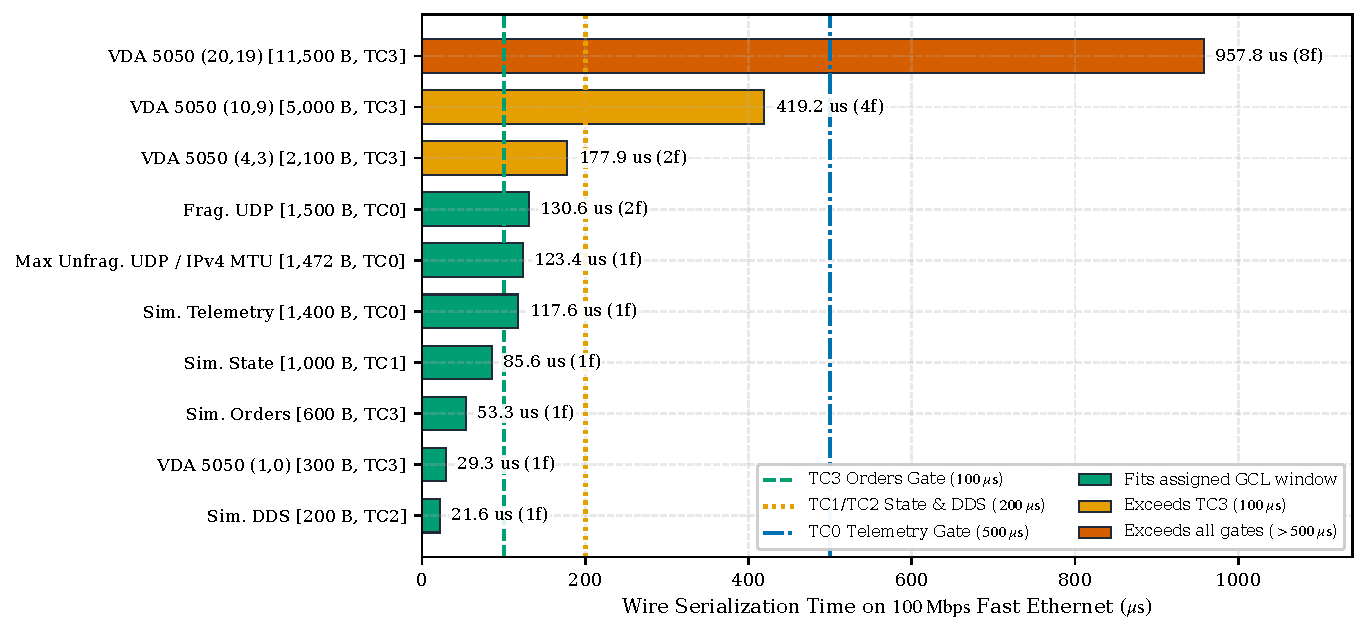
\includegraphics[width=0.92\textwidth]{images/pdf/fig_vda_gcl.pdf}
\caption{Wire serialization time at \qty{100}{\mbps} across simulated single-frame classes, the \qty{1472}{\byte} maximum unfragmented UDP / IPv4 MTU boundary, \qty{1500}{\byte} fragmented UDP, and illustrative rounded VDA~5050 multi-node surrogates (informed by Wagner et al.~\cite{11511549}, where tuple labels $(n, e)$ denote $(\text{nodes}, \text{edges})$ of linear path graphs) relative to the IEEE~802.1Qbv TC3 (\qty{100}{\micro\second}), TC1/TC2 (\qty{200}{\micro\second}), and TC0 (\qty{500}{\micro\second}) gate windows.}
\label{fig:vda_gcl}
\end{figure}

\subsection{Wireless Airtime Lower Bound and Single-Slot TDMA Superframe Feasibility}
\label{sec:analytical_wireless}

In IEEE~802.11g (ERP-OFDM with $\tau_{\mathrm{slot}} = \qty{9}{\micro\second}$, $\mathrm{SIFS} = \qty{10}{\micro\second}$, $\mathrm{DIFS} = \qty{28}{\micro\second}$, $\mathbb{E}[\mathrm{CW}_{\min}] = \qty{67.5}{\micro\second}$, $\qty{20}{\micro\second}$ physical preamble, and $\qty{6}{\micro\second}$ 2.4\,GHz signal extension per frame), collision-free scheduled airtime (DIFS included, zero contention backoff) requires \qty{258}{\micro\second} per \qty{1000}{\byte} State exchange and \qty{198}{\micro\second} per \qty{600}{\byte} Orders exchange at \qty{54}{\mbps} PHY, rising to \qty{814}{\micro\second} and \qty{550}{\micro\second} at \qty{12}{\mbps} PHY. At \qty{10}{\hertz} uplink State and \qty{5}{\hertz} downlink Orders per AMR, collision-free scheduled utilization equals \qty{3.57}{\milli\second\per\second} per AMR at \qty{54}{\mbps} ($\rho_{\mathrm{air,sched}} = \qty{14.3}{\percent}$ at $\Namr=40$, \qty{28.6}{\percent} at $\Namr=80$) and \qty{10.89}{\milli\second\per\second} per AMR at \qty{12}{\mbps} ($\rho_{\mathrm{air,sched}} = \qty{43.6}{\percent}$ at $\Namr=40$, \qty{87.1}{\percent} at $\Namr=80$). Under IEEE~802.11g CSMA/CA, adding the exact zero-collision backoff floor ($\mathbb{E}[\mathrm{CW}_{\min}] = \qty{67.5}{\micro\second}$ beyond DIFS prior to retransmissions) increases minimum airtime to \qty{325.5}{\micro\second} / \qty{265.5}{\micro\second} (\qty{4.58}{\milli\second\per\second} per AMR; $\rho_{\mathrm{air,CSMA}} = \qty{18.3}{\percent}$ at $\Namr=40$ and \qty{36.7}{\percent} at $\Namr=80$ at \qty{54}{\mbps}) and \qty{881.5}{\micro\second} / \qty{617.5}{\micro\second} (\qty{11.90}{\milli\second\per\second} per AMR; $\rho_{\mathrm{air,CSMA}} = \qty{47.6}{\percent}$ at $\Namr=40$ and \qty{95.2}{\percent} at $\Namr=80$ at \qty{12}{\mbps}), bringing \qty{12}{\mbps} CSMA/CA near saturation even before collision backoff escalations.

\begin{table}[!tb]
\centering
\scriptsize
\setlength{\tabcolsep}{2.0pt}
\caption{Locked analytical timing geometry of the \texttt{ScheduledDcf} TDMA superframe ($\mathrm{Occ} = \Namr \tau_{\mathrm{AMR}} + K \tau_{\mathrm{AP}}$).}
\label{tab:tdma_feasibility}
\begin{tabular}{@{}r r r r r r c r r r r r c@{}}
\toprule
 & \multicolumn{6}{c}{\textbf{54 Mbps ($\tau_{\mathrm{AMR}} = \tau_{\mathrm{AP}} = \qty{400}{\micro\second}$)}} & \multicolumn{6}{c}{\textbf{12 Mbps ($\tau_{\mathrm{AMR}} = \qty{850}{\micro\second},\; \tau_{\mathrm{AP}} = \qty{560}{\micro\second}$)}} \\
\cmidrule(lr){2-7} \cmidrule(lr){8-13}
\textbf{$\Namr$} & \textbf{$K$} & \textbf{Occ (ms)} & \textbf{$\Tsuper$ (ms)} & \textbf{Idle (ms)} & \textbf{$\rho_{\mathrm{SF}}$} & \textbf{$\le \qty{50}{\milli\second}$} & \textbf{$K$} & \textbf{Occ (ms)} & \textbf{$\Tsuper$ (ms)} & \textbf{Idle (ms)} & \textbf{$\rho_{\mathrm{SF}}$} & \textbf{$\le \qty{50}{\milli\second}$} \\
\midrule
5  & 1  & 2.40  & 3  & 0.60 & 80.0\% & Feasible & 1  & 4.81  & 6  & 1.19 & 80.2\% & Feasible \\
10 & 1  & 4.40  & 5  & 0.60 & 88.0\% & Feasible & 1  & 9.06  & 10 & 0.94 & 90.6\% & Feasible \\
20 & 2  & 8.80  & 9  & 0.20 & 97.8\% & Feasible & 3  & 18.68 & 20 & 1.32 & 93.4\% & Feasible \\
40 & 8  & 19.20 & 20 & 0.80 & 96.0\% & Feasible & 10 & 39.60 & 42 & 2.40 & 94.3\% & Feasible \\
80 & 39 & 47.60 & 48 & 0.40 & 99.2\% & Feasible & 39 & 89.84 & 90 & 0.16 & 99.8\% & \textbf{Exceeds} \\
\bottomrule
\end{tabular}
\end{table}

\begin{figure}[!tb]
\centering
\begin{tikzpicture}[
    scale=0.88, transform shape,
    font=\scriptsize,
    slot/.style={draw, rectangle, thick, minimum height=0.68cm, align=center}
]
    % Panel A: TAS GCL (clean +0.58 cm clearance above Panel B title)
    \node[anchor=west, font=\footnotesize\bfseries] at (0, 3.73) {(A) IEEE 802.1Qbv TAS Gate Control List (GCL) Cycle ($T_{\mathrm{GCL}} = \qty{1.0}{\milli\second} = \qty{1000}{\micro\second}$, Cells 5 \& 6)};
    \draw[slot, fill=cWlan!16]  (0.0, 2.40) rectangle (1.42, 3.08);
    \draw[slot, fill=orange!18] (1.42, 2.40) rectangle (4.26, 3.08) node[midway] {\textbf{TC2: DDS}\\$[100, 300)\,\mu\text{s}$};
    \draw[slot, fill=cSw!14]    (4.26, 2.40) rectangle (7.10, 3.08) node[midway] {\textbf{TC1: State}\\$[300, 500)\,\mu\text{s}$};
    \draw[slot, fill=cTeal!15]  (7.10, 2.40) rectangle (14.20, 3.08) node[midway, align=center] {\textbf{TC0: Telemetry} ($[500, 1000)\,\mu\text{s}$)\\4 frames/ms $\Rightarrow \qty{44.8}{\mbps}$ cap};
    \draw[{Stealth[length=1.4mm]}-, thick, cWlan!90!black] (0.71, 3.10) -- (1.05, 3.35) node[right, text=black, fill=white, inner sep=1pt] {\textbf{TC3: Orders} $[0, 100)\,\mu\text{s}$};
    \foreach \x/\t in {0.0/0, 1.42/100, 4.26/300, 7.10/500, 14.20/1000\,\mu\text{s}} {
        \draw[thick] (\x, 2.40) -- (\x, 2.26) node[below] {$\t$};
    }

    % Panel B: Exact ScheduledDcf layout at N=80, 12M
    \node[anchor=west, font=\footnotesize\bfseries] at (0, 1.26) {(B) \texttt{ScheduledDcf} TDMA Superframe at $\Namr=80,\; \qty{12}{\mbps}$ ($\Tsuper = \qty{90}{\milli\second}$, exact \texttt{omnetpp.ini} slot layout)};
    % 90 ms -> 14.2 cm (0.15778 cm/ms): 49.30ms=7.778, 50ms=7.889, 68.00ms=10.729, 89.84ms=14.175, 90.00ms=14.20
    \draw[slot, fill=cSw!15]    (0.0, -0.05) rectangle (7.78, 0.65) node[midway] {\texttt{amr[0..57]} ($\le D=\qty{50}{\milli\second}$)\\$58 \times \qty{850}{\micro\second} = \qty{49.30}{\milli\second}$};
    \draw[slot, fill=orange!18] (7.78, -0.05) rectangle (10.73, 0.65) node[midway] {\texttt{amr[58..79]}\\\qty{18.70}{\milli\second}};
    \draw[slot, fill=cWlan!18]  (10.73, -0.05) rectangle (14.17, 0.65) node[midway] {\textbf{Merged AP ($K{=}39$)}\\$39 \times \qty{560}{\micro\second} = \qty{21.84}{\milli\second}$};
    \draw[slot, fill=gray!25]   (14.17, -0.05) rectangle (14.20, 0.65);

    \draw[thick, red!80!black, dashed] (7.89, -0.25) -- (7.89, 0.78);
    \node[above, fill=white, inner sep=1pt, text=red!80!black] at (7.89, 0.78) {$D = \qty{50}{\milli\second}$};
    \draw[{Stealth[length=1.4mm]}-, thick, gray!75!black] (14.185, 0.66) -- (13.35, 0.90) node[left, text=black, fill=white, inner sep=1pt] {Idle: \qty{0.16}{\milli\second}};

    \foreach \x/\t in {0.0/0, 7.78/49.30, 10.73/68.00, 14.20/90.00\,\text{ms}} {
        \draw[thick] (\x, -0.05) -- (\x, -0.19) node[below] {$\t$};
    }
\end{tikzpicture}
\caption{Deterministic time-triggered schedules: (A)~IEEE~802.1Qbv \qty{1}{\milli\second} Gate Control List cycle; (B)~\texttt{ScheduledDcf} TDMA superframe at $(\Namr=80,\; \qty{12}{\mbps},\; \Tsuper=\qty{90}{\milli\second})$, showing \texttt{amr[0..57]} completing within $D=\qty{50}{\milli\second}$, the trailing $22$ AMRs (\texttt{amr[58..79]}), and the contiguous $39$-slot merged AP block (\qty{21.84}{\milli\second}) prior to the \qty{0.16}{\milli\second} ms-alignment idle margin.}
\label{fig:timing_diagrams}
\end{figure}

In Cells~2, 4, and 6, \texttt{ScheduledDcf} replaces random backoff with a static, conflict-free TDMA superframe computed via 64-bit integer fixed-point simulation ticks (\texttt{simtime\_t::raw()}) to eliminate floating-point drift, anchored at a fixed \texttt{cyclePhaseOffset = 0} relative to the TAS GCL. As detailed in \Cref{tab:tdma_feasibility} and \Cref{fig:timing_diagrams}B, each AMR receives one uplink slot ($\tau_{\mathrm{AMR}} = \qty{400}{\micro\second}$ at \qty{54}{\mbps}, $\qty{850}{\micro\second}$ at \qty{12}{\mbps}) followed by a contiguous $K$-slot merged downlink AP block ($K \in \{1, 1, 2, 8, 39\}$ at \qty{54}{\mbps}; $K \in \{1, 1, 3, 10, 39\}$ at \qty{12}{\mbps}), configured on integer-millisecond superframes with \qtyrange{0.16}{2.40}{\milli\second} of deliberate idle slack. In the baseline schedule configuration, $K$ is provisioned by mean rate matching ($K/\Tsuper \ge 5\Namr$ while holding $\Tsuper \le \qty{90}{\milli\second}$ at $(\Namr=80,\; \qty{12}{\mbps})$ so per-AMR State service remains at $1/\qty{90}{\milli\second} = \qty{11.11}{\hertz} > \qty{10}{\hertz}$ and avoids persistent 2-packet State buildup).

Because downlink Orders arrivals are Poisson with mean $\lambda = 5\Namr\Tsuper$ per cycle, this mean-rate rule leaves generous burst headroom at \qty{54}{\mbps} ($K=8$ vs.\ $\lambda=4.0$, $+2.0\sigma$ at $\Namr=40$; $K=39$ vs.\ $\lambda=19.2$, $+4.5\sigma$ at $\Namr=80$), but intentionally provisions only $\approx +0.5\sigma$ margin at \qty{12}{\mbps}:
\begin{itemize}[leftmargin=1.8em]
    \item \textbf{Tight AP Provisioning at $(\Namr=40,\; \qty{12}{\mbps},\; \Tsuper=\qty{42}{\milli\second})$:} Because $\Tsuper = \qty{42}{\milli\second} < D_{\mathrm{state}} = \qty{50}{\milli\second}$, TDMA itself introduces zero uplink State misses: wired-isolated Cells~4 and~6 (802.1Q and TAS) preserve \qty{0.00}{\percent} State misses across all eight telemetry loads, whereas FIFO+TDMA (Cell~2) incurs wired switch overflow above \qty{85.0}{\mbps} (\qty{42.49}{\percent} in $R=22$ \texttt{supp-maxR}; \qty{42.40}{\percent} in \texttt{core-R3} at \qty{149.3}{\mbps}). On the downlink, however, $K=10$ ($\rho_{\mathrm{AP}} = \qty{84.0}{\percent}$, $\lambda = 8.40$ orders/cycle, $+0.55\sigma$) causes $\Pr[\mathrm{Pois}(8.40) > 10] = \qty{22.57}{\percent}$ of \emph{cycles} to overflow; at the packet level, the single-cycle overflow share is $\mathbb{E}[(X-10)^+]/8.40 = \qty{6.54}{\percent}$, and a stationary discrete-slot $M/D^{10}/1$ queueing evaluation with $\mathcal{U}(0, \qty{10}{\milli\second})$ NER tick slack yields $\MissA = \qty{6.70}{\percent}$ and $\MissB = \qty{4.59}{\percent}$ (closely matching the empirical 8-load mean penalty of \qty{4.68}{\percent} in Cells~2/4 and \qty{4.82}{\percent} across Cells~2/4/6). Increasing $K$ from $10$ to $12$ within the \emph{existing} \qty{2.40}{\milli\second} idle margin keeps $\Tsuper = \qty{42}{\milli\second}$ unchanged ($\rho_{\mathrm{AP}} = \qty{70.0}{\percent}$) and cuts $M/D^{12}/1$ Orders $\MissB$ to \qty{0.18}{\percent}.
    \item \textbf{Three-Part Orders and State Breakdown at $(\Namr=80,\; \qty{12}{\mbps},\; \Tsuper=\qty{90}{\milli\second})$:} On the uplink, a single slot every \qty{90}{\milli\second} forces $(90-50)/90 \approx \qty{44.4}{\percent}$ of uniform-phase State arrivals to exceed \qty{50}{\milli\second} ($\approx \qty{40}{\percent}$ after NER tick slack). On the downlink, locating the merged $K=39$ AP block ($\qty{21.84}{\milli\second}$, $\lambda = 36.0$, $\rho_{\mathrm{AP}} = \qty{92.3}{\percent}$, $+0.50\sigma$) at the end of the \qty{90}{\milli\second} cycle decomposes the observed Cell~2 Orders miss rate ($\MissA = \qty{39.18}{\percent}$, $\MissB = \qty{31.89}{\percent}$; matched by $M/D^{39}/1$ at $\qty{39.00}{\percent}$ and $\qty{31.98}{\percent}$) into three additive mechanisms: (i)~pure block-start phase wait for packets arriving in $[0, \qty{18.6}{\milli\second})$ before $t=\qty{68.0}{\milli\second}$ (\qty{20.77}{\pp} $\MissA$ / \qty{15.21}{\pp} $\MissB$, irreducible under any single contiguous trailing block regardless of $K$); (ii)~within-block serial service across $\approx 27.2$ frames at \qty{0.56}{\milli\second}/slot ($+5.87\text{ pp}\; \MissA$ / $+4.27\text{ pp}\; \MissB$); and (iii)~multi-cycle backlog carryover across consecutive cycles when \qty{27.37}{\percent} of cycles overflow ($3.36\%$ single-cycle packet overflow compounding at $\rho_{\mathrm{AP}}=\qty{92.3}{\percent}$ to add $+12.36\text{ pp}\; \MissA$ / $+12.50\text{ pp}\; \MissB$). Splitting the AP grant into two half-cycle sub-blocks ($\qty{46}{\milli\second}$ spacing) eliminates both the \qty{15.2}{\pp} block-start barrier and multi-cycle buildup (\Cref{sec:codesign_pilot}).
\end{itemize}

\subsection{Per-Class Offered Load versus Guaranteed Service Capacity}
\label{sec:capacity_proof}

Across discrete-event queuing and time-triggered schedules, \emph{rate sustainability} ($\rho_c = \lambda_c / \mu_c < 1$, ensuring finite steady-state queues without monotonic buffer divergence) is necessary but not sufficient for \emph{deadline compliance} ($\MissA(D_c), \MissB(D_c) \le \qty{1.0}{\percent}$). A class can operate at strictly sustainable utilization ($\rho_c < 1$) and still violate its deadline budget due to finite-buffer burst overflow, worst-case gate/superframe phase wait, or multi-domain delay addition. Conversely, an intentionally overloaded elastic stream ($\rho_c > 1$) collapses only itself when isolated by strict priority or exclusive gating, but destabilizes companion classes when sharing a FIFO drop-tail buffer or contention medium. \Cref{tab:capacity_proof} evaluates offered rates $\lambda_c$ against exact analytical guaranteed or residual service rates $\mu_c$ across every tested wired and wireless configuration in the $80$-point design.

\begin{table}[!tb]
\centering
\scriptsize
\setlength{\tabcolsep}{2.2pt}
\caption{Per-class offered load ($\lambda_c$) versus guaranteed or residual service capacity ($\mu_c$) across all tested wired (\qty{100}{\mbps}) and wireless (\qtylist{54;12}{\mbps}) architectures, separating steady-state rate sustainability ($\rho_c < 1$) from end-to-end deadline compliance ($D_c$).}
\label{tab:capacity_proof}
\begin{tabularx}{\textwidth}{@{}P{1.80cm} P{1.75cm} r r r P{3.00cm} Y@{}}
\toprule
\textbf{Domain /} & \textbf{Class} & \textbf{Offered} & \textbf{Service} & \textbf{Max} & \textbf{Rate Sustainable} & \textbf{Deadline Compliance ($D_c$)} \\
\textbf{Config} & \textbf{(Port)} & \textbf{$\lambda_c$} & \textbf{$\mu_c$} & \textbf{$\rho_c$} & \textbf{($\rho_c < 1$)} & \\
\midrule
\multicolumn{7}{@{}l@{}}{\textbf{Panel A: Wired Fast Ethernet Backbone (\qty{100}{\mbps}; \texttt{eth[0]} +\qty{70}{\byte} C-tagged, \texttt{eth[1]} +\qty{66}{\byte} untagged)}} \\
\midrule
FIFO / 802.1Q & Orders (\texttt{eth[1]}) & 25..400\,fps & 18,768\,fps & 2.1\% & All 80 pts (dedic.\ link) & Compliant (\texttt{eth[1]} delay $\le \qty{0.1}{\milli\second}$) \\
Uniform TAS & Orders (\qty{100}{\micro\second}) & 25..400\,fps & 1,000\,fps & 40.0\% & All 80 pts (\qty{4.80}{\mbps} cap) & Compliant (\texttt{eth[1]} gate wait $\le \qty{1}{\milli\second}$) \\
FIFO (C1, C2) & DDS / State (\texttt{eth[0]}) & 400 / 50..800\,fps & 100\,M shared & 164.5\% & $\ltel \le \qty{85.0}{\mbps}$ (tot.\ $\le \qty{97.0}{\mbps}$) & DDS $\MissA$ fails at $(\Namr{=}80,\; \qty{85}{\mbps})$ (\qty{9.41}{\milli\second} drain); both fail $\ge \qty{95}{\mbps}$ \\
802.1Q (C3, C4) & DDS (TC2) & 400\,fps & 46,296\,fps & 0.86\% & All 80 pts (top on \texttt{eth[0]}) & Compliant across all 80 pts (\qty{0.00}{\percent}) \\
802.1Q (C3, C4) & State (TC1) & 50..800\,fps & 11,581\,fps\textsuperscript{a} & 6.91\% & All 80 pts (\qty{99.14}{\mbps} resid.) & Wired-compliant across all 80 pts \\
Uniform TAS & DDS (\qty{200}{\micro\second}) & 400\,fps & 9,000\,fps\textsuperscript{b} & 4.44\% & All 80 pts (\qty{14.40}{\mbps} cap) & Compliant across all 80 pts (\qty{0.00}{\percent}) \\
Uniform TAS & State (\qty{200}{\micro\second}) & 50..800\,fps & 2,000\,fps & 40.0\% & All 80 pts (\qty{16.00}{\mbps} cap) & Wired-compliant across all 80 pts \\
FIFO / 802.1Q & Tel.\ (TC0) & 2.0k..13.3k\,fps & 7,848..8,394\,fps\textsuperscript{a} & 169.9\% & $\ltel \le \qty{85.0}{\mbps}$ ($\le \qty{96.7}{\percent}$) & 802.1Q 20-pkt burst drops $\le \qty{0.46}{\percent}$ at \qtyrange{74.7}{85.0}{\mbps}; fails $\ge \qty{95}{\mbps}$ \\
Uniform TAS & Tel.\ (\qty{500}{\micro\second}) & 2.0k..13.3k\,fps & 4,000\,fps & 333.3\% & $\ltel = \qty{22.4}{\mbps}$ ($\rho = \qty{50}{\percent}$) & Fails for all $\ltel \ge \qty{45.0}{\mbps}$ (\qty{44.80}{\mbps} cap) \\
Rebal.\ TAS\textsuperscript{c} & Tel.\ (\qty{720}{\micro\second}) & 4.0k..7.6k\,fps & 6,000\,fps & 126.5\% & $\ltel \le \qty{60.0}{\mbps}$ (\qty{89.2}{\percent} at \qty{60}{\mbps}) & Clears \qtyrange{45}{60}{\mbps} ($\le \qty{0.13}{\percent}$, \qty{67.20}{\mbps} cap); fails $\ge \qty{74.7}{\mbps}$ \\
\midrule
\multicolumn{7}{@{}l@{}}{\textbf{Panel B: Wireless IEEE 802.11g Radio Link (UL State 10\,fps/AMR + DL Orders 5$\Namr$\,fps)}} \\
\midrule
CSMA \qty{54}{\mbps} & State + Orders & 75..1,200\,fps & Shared\textsuperscript{d} & 36.7\%\textsuperscript{d} & All $\Namr \le 80$ (unsaturated) & Compliant across all $\Namr \le 80$ (\qty{0.00}{\percent}) \\
CSMA \qty{12}{\mbps} & State + Orders & 75..1,200\,fps & Shared\textsuperscript{d} & 95.2\%\textsuperscript{d} & $\Namr \le 40$ ($\le \qty{47.6}{\percent}$); AP starves $N{=}80$ & Compliant for $\Namr \le 40$; $N{=}80$ DL TXOP share \qty{1.2}{\percent} vs.\ \qty{33.3}{\percent} req.\ + UL collapse \\
TDMA \qty{54}{\mbps} & State / Orders & \begin{tabular}[t]{@{}r@{}}10/AMR;\\25..400\,fps\end{tabular} & \begin{tabular}[t]{@{}r@{}}20.8..333/AMR;\\200..813\,fps\end{tabular} & \begin{tabular}[t]{@{}r@{}}48.0 /\\50.0\%\end{tabular} & All $\Namr \le 80$ (\qty{0.00}{\percent} drop) & Wirelessly compliant ($\Tsuper \le \qty{48}{\milli\second}$); C2 fails at $(\Namr{=}80,\; \qty{149.3}{\mbps})$ \\
TDMA \qty{12}{\mbps} & State (UL) & 10.0\,fps/AMR & 11.1..166.7/AMR & 90.0\% & All $\Namr \le 80$ (\qty{0.00}{\percent} drop) & Compliant $\Namr \le 40$ ($\Tsuper \le \qty{42}{\milli\second}$); fails at $\Namr{=}80$ ($\Tsuper{=}\qty{90}{\milli\second} > \qty{50}{\milli\second}$) \\
TDMA \qty{12}{\mbps} & Orders (DL) & 25..400\,fps & 100.0..433.3\,fps & 92.3\% & All $\Namr \le 80$ (\qty{0.00}{\percent} drop) & Fails at $N{=}40$ ($K{=}10$, \qtyrange{4.7}{5.1}{\percent}) and $N{=}80$ ($K{=}39$, \qtyrange{31.9}{32.6}{\percent}) \\
\bottomrule
\end{tabularx}
\par\vspace{2pt}
\raggedright\scriptsize
\textsuperscript{a}\,Residual link rate after higher-priority \texttt{eth[0]} traffic (\qty{99.14}{\mbps} after \qty{0.864}{\mbps} DDS; \qtyrange{92.29}{98.71}{\mbps} after DDS+State across $\Namr \in \{5, 10, 20, 40, 80\}$). \textsuperscript{b}\,Nine frames/ms under wire accounting (\qty{10000}{fps} L2). \textsuperscript{c}\,Port-specific \texttt{eth[0]} schedule ($\text{TC2}{=}\qty{100}{\micro\second}$, $\text{TC1}{=}\qty{180}{\micro\second}$, $\text{TC0}{=}\qty{720}{\micro\second}$) preserving \qty{10}{\percent} DDS and \qty{20}{\percent} State utilization at $\Namr=40$ ($\le \qty{40}{\percent}$ through $\Namr=80$); verified in \Cref{tab:gcl_pilot} (\qty{0.00}{\percent} / \qty{0.13}{\percent} at \qtylist{45;60}{\mbps} vs.\ \qty{10.15}{\percent} / \qty{21.00}{\percent} above \qty{67.20}{\mbps}). \textsuperscript{d}\,Zero-collision CSMA airtime utilization floor $\rho_{\mathrm{air,CSMA}}$ (\Cref{sec:analytical_wireless}); exact CSMA capacity depends on contention and SNIR capture.
\end{table}

Two sharp capacity-versus-deadline gaps in \Cref{tab:capacity_proof} govern the empirical behaviors analyzed in \Cref{sec:results}. On the wired trunk, Best-Effort FIFO retains $\rho < 1$ through $\ltel = \qty{85.0}{\mbps}$, yet its \qty{9.41}{\milli\second} drain bound already causes Watchdog $\MissA$ misses for \qty{5}{\milli\second} DDS at $(\Namr=80,\; \qty{85.0}{\mbps})$; conversely, 802.1Q isolates critical queues across all 80 points while uniform TAS (\qty{500}{\micro\second} TC0) becomes rate-unstable for Telemetry at every $\ltel \ge \qty{45.0}{\mbps}$. On the \qty{12}{\mbps} radio link, TDMA maintains strict $\rho < 1$ and zero physical drops across all fleet sizes up to $\Namr=80$, yet still fails the \qty{50}{\milli\second} deadline on downlink Orders at $\Namr=40$ (mean-rate AP provisioning $\rho_{\mathrm{AP}} = \qty{84.0}{\percent}$ under Poisson bursts) and on both State and Orders at $\Namr=80$ ($\Tsuper = \qty{90}{\milli\second} > \qty{50}{\milli\second}$); meanwhile, CSMA/CA loses rate stability on downlink Orders at $\Namr=80,\; \qty{12}{\mbps}$ because symmetric backoff grants the AP only $1/(80+1) = \qty{1.2}{\percent}$ transmit opportunities against a \qty{33.3}{\percent} downlink frame share requirement.

% =============================================================================
\section{Empirical Results by Research Question}
\label{sec:results}

\Cref{tab:rq_summary} summarizes the main quantitative answers to RQ-(i) through RQ-(iii) alongside supporting diagnostics and lookup interpolation results across the full $80$-point grid.

\begin{table}[!tb]
\centering
\footnotesize
\caption{Summary of research questions, operating regimes across the $80$-point factorial grid (\num{6924} paired runs plus $23$ post-hoc Cell~1 collapse seeds), and primary evidence links.}
\label{tab:rq_summary}
\begin{tabularx}{\textwidth}{P{2.9cm} Y P{2.9cm}}
\toprule
\textbf{Question / Scope} & \textbf{Core Regime Finding} & \textbf{Primary Evidence} \\
\midrule
RQ-(i) Isolated upgrades & 802.1Q clears critical wired congestion above \qtyrange{85}{95}{\mbps} ($\GainP=\qty{+43.91}{\pp}$ $\MissB$ / \qty{+83.38}{\pp} Watchdog $\MissA$ on DDS), while the static uniform GCL caps Telemetry at \qty{44.8}{\mbps} ($\GainS=\qty{-33.93}{\pp}$; \qtyrange{56.0}{78.4}{\mbps} analytically under port-specific rebalancing, \qty{67.20}{\mbps} verified in \Cref{tab:gcl_pilot}). Under \qty{12}{\mbps} TDMA, tight AP slots induce $\Namr=40$ Orders carryover (\qty{-4.68}{\pp} $\MissB$ / \qty{-6.86}{\pp} $\MissA$ vs.\ Cell~1) and single-slot wait rescues $\Namr=80$ Orders (\qty{+63.07}{\pp} $\MissB$ / \qty{+56.15}{\pp} $\MissA$ 8-load mean) at the expense of uplink State. & \Cref{sec:rq1}; \Cref{tab:aggregate_performance,tab:deadline_spectrum}; \Cref{fig:isolated_upgrades,fig:unpooled_n80} \\
\addlinespace[2pt]
RQ-(ii) Cross-domain masking & Companion bottlenecks cap local gains (\texttt{eth[0]} vs.\ \texttt{eth[1]}); under wired saturation at $\Namr=80,\; \qty{54}{\mbps}$, adding TDMA ($\Tsuper=\qty{48}{\milli\second}$) induces a \qty{-3.13}{\pp} interaction (\qty{0}{\percent} in either isolated domain), and at \qty{12}{\mbps} lifts the conditional delivered State late share from \qty{39.91}{\percent} to \qty{49.83}{\percent}. Across all $176$ paired $(\Namr=80,\; \qty{12}{\mbps})$ CSMA runs, Cell~5 vs.\ Cell~3 State $\MissB$ shows zero systematic bias (median diff \qty{+0.00}{\pp}, Wilcoxon $p=0.486$; $13$ vs.\ $13$ collapses). & \Cref{sec:rq2}; \Cref{tab:domain_delay_decomp,tab:selected_points,tab:hypothesis_test}; \Cref{fig:domain_drops,fig:ecdf_n80,fig:domain_bars} \\
\addlinespace[2pt]
RQ-(iii) Dual-domain determinism & Under joint saturation, dual-domain Cells~4 and~6 are necessary for zero critical physical loss, though not sufficient at $\Namr=80,\; \qty{12}{\mbps}$. Under the distribution-free per-seed screen ($\max_r Y_r \le \qty{1.0}{\percent}$), Cells~4 and~6 pass all $24/24$ Confirmatory ($R=22$) points at \qty{54}{\mbps} and $5/24$ at \qty{12}{\mbps} ($29/48 = \qty{60.4}{\percent}$ Confirmatory; $61/80 = \qty{76.2}{\percent}$ $\MissB$ and $56/80 = \qty{70.0}{\percent}$ Watchdog $\MissA$/$\MissB$ across all $80$ points; $40/40$ at \qty{54}{\mbps} vs.\ $40/48$ Confirmatory and $72/80$ in Cells~3/5), requiring \qty{54}{\mbps} PHY or multi-slot access for $\le \qty{50}{\milli\second}$ compliance at $\Namr=80$. & \Cref{sec:rq3}; \Cref{tab:dual_stress_matrix,tab:migration_regimes,tab:conformance_summary}; \Cref{fig:conformance_bars,fig:migration_heatmaps} \\
\addlinespace[2pt]
Supporting studies & Unbiased Cell~1 confirmation seeds ($r=22..44$) record $0/23$ runaway collapses ($3/23$ stalls $\ge \qty{10}{\percent}$), while layout-clustered CSMA collapse spans $13/176$ runs (\qty{7.39}{\percent}) in Cells~3 and~5; TDMA caps delivered ZOH State staleness at $\le \qty{5}{\tick}$ (equal-scenario mean $\le \qty{0.11}{\tick}$ vs.\ up to \num{1913} ticks CSMA), 8-load PCHIP achieves matched critical-class MAE $\le \qty{3.11}{\pp}$, and targeted TDMA, port-specific GCL, and Cell~3 buffer-parity controls empirically isolate downlink, TC0 gating, and priority preemption limits. & \Cref{sec:supporting}; \Cref{tab:collapse_incidence,tab:ner_multirate,tab:pchip_loo,tab:codesign_pilot,tab:gcl_pilot,tab:bufparity_pilot}; \Cref{fig:wireless_diagnostics,fig:ner_interface} \\
\bottomrule
\end{tabularx}
\end{table}

\subsection{RQ-(i): Isolated Wired and Wireless Domain Upgrades}
\label{sec:rq1}

An isolated wired strict-priority upgrade eliminates switch queue drops for critical DDS and State traffic above the \qtyrange{85}{95}{\mbps} FIFO saturation bracket, whereas isolated single-slot TDMA rescues downlink Orders under $\Namr=80,\; \qty{12}{\mbps}$ contention at the expense of uplink State latency and $\Namr=40$ AP block spillover.

\begin{table}[!tb]
\centering
\scriptsize
\setlength{\tabcolsep}{1.6pt}
\caption{Aggregate performance across the six factorial cells on the balanced 4-load \texttt{core-R3} pool ($40$ points) and the full $80$-point \texttt{supp-maxR} pool ($\MissB$ primary tick metric; KILL classes DDS and Orders additionally list Watchdog-enforced unavailability $\MissA$ in parentheses; $p_{99}$ reports scenario-level 99th-percentile latency across \texttt{supp-maxR}).}
\label{tab:aggregate_performance}
\begin{tabular}{@{}l l r r r r r r r@{}}
\toprule
\textbf{Class} & \textbf{Cell} & \multicolumn{2}{c}{\textbf{core-R3 (\%)}} & \multicolumn{4}{c}{\textbf{supp-maxR (80 Pts, \%)}} & \textbf{$p_{99}$ (ms)} \\
\cmidrule(lr){3-4} \cmidrule(lr){5-8}
\textbf{($D_c$)} & \textbf{(Arch.)} & \textbf{$\MissB$ ($\MissA$)} & \textbf{$\ploss$} & \textbf{$\MissB$ ($\MissA$)} & \textbf{$\ploss$} & \textbf{Max $\MissB$} & \textbf{$>\qty{1}{\percent}$} & \textbf{Mean / Max} \\
 & & & & & & \textbf{($\MissA$)} & & \\
\midrule
DDS & C1 (FIFO+CSMA) & 24.30 (45.56) & 13.78 & 18.67 (35.44) & 9.58 & \begin{tabular}[t]{@{}r@{}}72.36\\(100.0)\end{tabular} & \begin{tabular}[t]{@{}r@{}}30/80\\(32/80)\end{tabular} & 4.39 / 9.56 \\
(\qty{5}{\milli\second}) & C2 (FIFO+TDMA) & 24.26 (45.54) & 13.76 & 18.65 (35.44) & 9.58 & \begin{tabular}[t]{@{}r@{}}72.33\\(100.0)\end{tabular} & \begin{tabular}[t]{@{}r@{}}30/80\\(32/80)\end{tabular} & 4.39 / 9.56 \\
 & C3 / C4 (802.1Q) & \textbf{0.00} (0.00) & \textbf{0.00} & \textbf{0.00} (0.00) & \textbf{0.00} & \textbf{0.00} (0.00) & \begin{tabular}[t]{@{}r@{}}\textbf{0/80}\\(0/80)\end{tabular} & 0.29 / 0.40 \\
 & C5 / C6 (TAS) & \textbf{0.00} (0.00) & \textbf{0.00} & \textbf{0.00} (0.00) & \textbf{0.00} & \textbf{0.00} (0.00) & \begin{tabular}[t]{@{}r@{}}\textbf{0/80}\\(0/80)\end{tabular} & 0.90 / 0.96 \\
\midrule
State & C1 (FIFO+CSMA) & 11.82 & 11.45 & 8.89 & 8.01 & 45.70 & 35/80 & 280.39 / 5367.31 \\
(\qty{50}{\milli\second}) & C2 (FIFO+TDMA) & 15.55 & 11.51 & 12.11 & 8.01 & 70.98 & 35/80 & 29.15 / 98.95 \\
 & C3 (802.1Q+CSMA) & 0.39 & 0.01 & 0.95 & 0.04 & 18.89 & 8/80 & 276.25 / 5367.08 \\
 & C4 (802.1Q+TDMA) & 3.99 & \textbf{0.00} & 3.99 & \textbf{0.00} & 39.98 & 8/80 & 25.64 / 90.05 \\
 & C5 (TAS+CSMA) & 0.42 & 0.01 & 1.02 & 0.04 & 18.02 & 8/80 & 324.98 / 5682.70 \\
 & C6 (TAS+TDMA) & 4.03 & \textbf{0.00} & 4.05 & \textbf{0.00} & 40.53 & 8/80 & 26.14 / 90.40 \\
\midrule
Orders & C1 / C3 (CSMA) & 9.40 (9.45) & 1.02 & 9.49 (9.53) & 1.58 & \begin{tabular}[t]{@{}r@{}}96.25\\(96.56)\end{tabular} & \begin{tabular}[t]{@{}r@{}}8/80\\(8/80)\end{tabular} & 86.31 / 972.66 \\
(\qty{50}{\milli\second}) & C5 (TAS+CSMA) & 9.53 (9.56) & 0.96 & 9.53 (9.56) & 1.63 & \begin{tabular}[t]{@{}r@{}}96.47\\(96.67)\end{tabular} & \begin{tabular}[t]{@{}r@{}}8/80\\(8/80)\end{tabular} & 86.51 / 948.46 \\
 & C2 / C4 (TDMA) & 3.64 (4.64) & \textbf{0.00} & 3.70 (4.70) & \textbf{0.00} & \begin{tabular}[t]{@{}r@{}}32.03\\(39.36)\end{tabular} & \begin{tabular}[t]{@{}r@{}}16/80\\(17/80)\end{tabular} & 34.52 / 109.83 \\
 & C6 (TAS+TDMA) & 3.75 (4.78) & \textbf{0.00} & 3.80 (4.82) & \textbf{0.00} & \begin{tabular}[t]{@{}r@{}}32.64\\(39.96)\end{tabular} & \begin{tabular}[t]{@{}r@{}}16/80\\(17/80)\end{tabular} & 34.98 / 110.08 \\
\midrule
Telemetry & C1 (FIFO+CSMA) & 10.13 & 10.13 & 7.06 & 7.06 & 38.99 & 30/80 & 4.56 / 9.76 \\
(\qty{100}{\milli\second}) & C2 (FIFO+TDMA) & 10.13 & 10.13 & 7.06 & 7.06 & 39.00 & 30/80 & 4.57 / 9.76 \\
 & C3 (802.1Q+CSMA) & 10.72 & 10.72 & 7.48 & 7.48 & 41.13 & 32/80 & 1.85 / 3.17 \\
 & C4 (802.1Q+TDMA) & 10.73 & 10.73 & 7.49 & 7.49 & 41.13 & 32/80 & 1.86 / 3.20 \\
 & C5 / C6 (TAS) & 40.70 & 40.70 & 37.18 & 37.18 & 70.00 & 70/80 & 4.84 / 5.47 \\
\bottomrule
\end{tabular}
\end{table}

\begin{figure}[!tb]
\centering
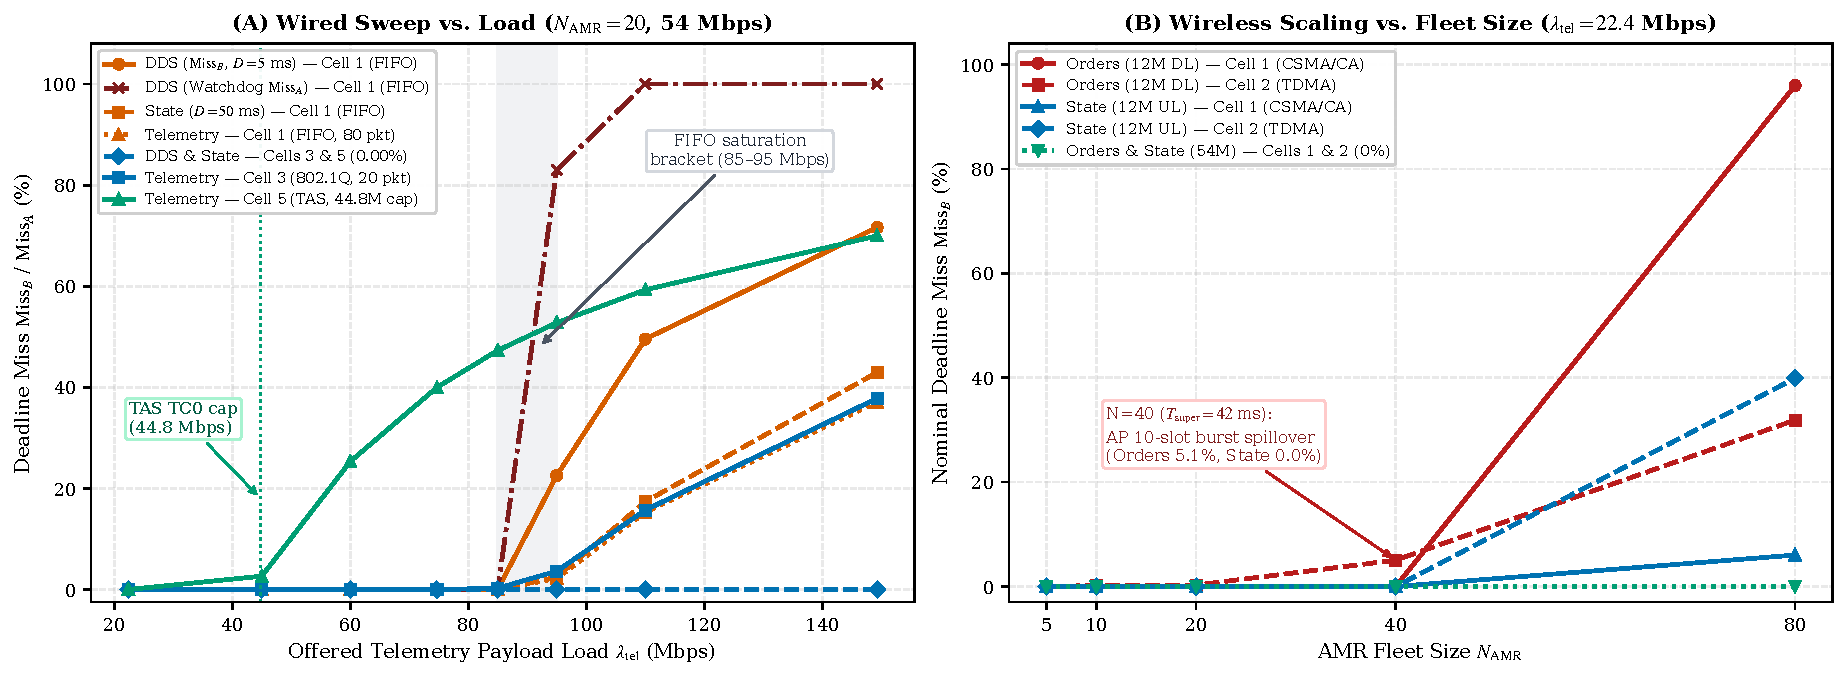
\includegraphics[width=0.95\textwidth]{images/pdf/fig_isolated_upgrades.pdf}
\caption{Isolated wired and wireless transition regimes: (A)~wired saturation sweep across the eight-load knee-R3 grid ($\Namr=20,\; \qty{54}{\mbps}$), bracketing FIFO saturation within \qtyrange{85}{95}{\mbps}, overlaying continuous Watchdog $\MissA$ for FIFO DDS (dashed, reaching \qty{100.0}{\percent} at \qty{149.3}{\mbps}), and confirming the \qty{44.8}{\mbps} TAS TC0 cap; (B)~wireless fleet scaling at $\ltel=\qty{22.4}{\mbps}$ across $\Namr \in \{5..80\}$, highlighting AP 10-slot spillover on Orders at $(\Namr=40,\; \qty{12}{\mbps})$ where uplink State remains at \qty{0.00}{\percent}.}
\label{fig:isolated_upgrades}
\end{figure}

\paragraph{Isolated Wired Upgrade and the \qtyrange{85}{95}{\mbps} FIFO Saturation Bracket.}
Across the 8-load knee-R3 sweep at unsaturated wireless capacity (\Cref{fig:isolated_upgrades}A and \Cref{tab:aggregate_performance}), Best-Effort FIFO (Cells~1 and 2) maintains $\MissB = \qty{0.00}{\percent}$ across all five telemetry loads up to $\ltel = \qty{85.0}{\mbps}$ for $\Namr \le 20$ (with minor onset of \qty{0.04}{\percent} at $\Namr=40$ and \qty{0.75}{\percent} at $\Namr=80$; under continuous Watchdog $\MissA$, those two $\Namr=80$ points at \qty{85.0}{\mbps} already reach \qtyrange{3.94}{9.17}{\percent} because FIFO queue tails cross \qty{5}{\milli\second} before crossing the \qty{10}{\milli\second} tick slack, explaining why $32/80$ FIFO points exceed \qty{1}{\percent} under $\MissA$ versus $30/80$ under $\MissB$). Including Ethernet framing plus State and DDS traffic, \qty{85.0}{\mbps} of telemetry payload corresponds to \qtyrange{91.0}{93.6}{\mbps} of aggregate wire load on \texttt{eth[0]} for $\Namr \in \{10, 20, 40\}$. Between $\ltel = \qty{85.0}{\mbps}$ and \qty{95.0}{\mbps} (\qtyrange{101.4}{104.0}{\mbps} total wire load), \texttt{eth[0]} crosses its \qty{100}{\mbps} capacity: in Cell~1 at \qty{54}{\mbps} PHY, DDS $\MissB(\qty{5}{\milli\second})$ jumps from \qty{0.00}{\percent} at \qty{85.0}{\mbps} (\qty{0.04}{\percent} at $\Namr=40$, \qty{0.75}{\percent} at $\Namr=80$) to \qtyrange{18.62}{31.18}{\percent} across $\Namr \in \{10,20,40\}$ at \qty{95.0}{\mbps} (\qty{15.83}{\percent} at $\Namr=5$; \qty{38.34}{\percent} at $\Namr=80$) and \qtyrange{70.96}{72.29}{\percent} across all five fleet sizes at \qty{149.3}{\mbps} (reaching \qty{100.0}{\percent} Watchdog $\MissA$ because every delivered frame exceeds \qty{5}{\milli\second} in \Cref{eq:fifo_drain}). Because our load grid samples \qty{85.0}{\mbps} and \qty{95.0}{\mbps}, the empirical data brackets the wired saturation onset within \qtyrange{85}{95}{\mbps} of telemetry payload.

Upgrading the switch from FIFO to IEEE~802.1Q Strict Priority (Cells~3 and 4) isolates DDS (TC2) and State (TC1) in dedicated priority queues ahead of Telemetry (TC0), eliminating \qty{100}{\percent} of wired switch drops for DDS and State ($p_{\mathrm{drop,Q}} = \qty{0.00}{\percent}$ on TC1 and TC2, while background Telemetry TC0 still drops up to \qty{41.13}{\percent} under 802.1Q and \qty{70.00}{\percent} under TAS). Across the $34$ active wired-bottleneck points ($\ltel \ge \qty{85.0}{\mbps}$), 802.1Q yields a paired priority gain of $\GainP = \qty{+43.91}{\pp}$ on DDS under $\MissB$ and $\qty{+83.38}{\pp}$ under continuous Watchdog $\MissA$ (and $\GainP = \qty{+20.61}{\pp}$ on State across the $28$ active State points), while reducing points exceeding \qty{1}{\percent} from $30/80$ ($\MissB$) or $32/80$ ($\MissA$) in Cells~1 and 2 to $0/80$ across Cells~3 through 6 under both metrics. In Cell~1 (FIFO) at $(\Namr=80,\; \qty{54}{\mbps},\; \qty{149.3}{\mbps})$, packet-level drops total \qty{52.68}{\percent} for DDS ($\MissB = \qty{72.29}{\percent}$, $\MissA = \qty{100.0}{\percent}$), \qty{43.06}{\percent} for State, and \qty{38.96}{\percent} for Telemetry. Rather than stemming from packet size inside the switch queue, this asymmetry arises from ingress \qty{100}{\mbps} link store-and-forward serialization breaking the Poisson-arrival assumption required for Poisson Arrivals See Time Averages (PASTA) in two additive ways: (1)~each station's \qty{100}{\mbps} ingress trunk serializes a \qty{1466}{\byte} untagged Telemetry frame in \qty{117.28}{\micro\second}, creating a self-spacing interval comparable to one \qty{117.60}{\micro\second} egress transmission on \texttt{eth[0]} so consecutive same-station Telemetry arrivals never stack within that slot, whereas independent AP uplink State frames face all four stations (\qty{43.06}{\percent} vs.\ \qty{38.96}{\percent}); and (2)~each station multiplexes \qty{266}{\byte} DDS (\qty{21.28}{\micro\second}) onto the same busy ($\approx \qty{39}{\percent}$) ingress NIC as Telemetry, causing queued DDS frames to enter the switch only \qty{21.28}{\micro\second} behind a Telemetry frame ($\ll \qty{117.60}{\micro\second}$ egress drain time) and strike the 80-packet FIFO buffer at peak occupancy (\qty{52.68}{\percent} loss; an independent store-and-forward discrete-event verification in \path{tool/verify_pasta_ingress.py} reproduces \qty{52.72}{\percent} / \qty{44.09}{\percent} / \qty{39.04}{\percent}, collapsing to near-uniform \qty{38.61}{\percent} / \qty{39.40}{\percent} / \qty{39.32}{\percent} when ingress serialization is removed).

\paragraph{Configuration-Dependent TAS Shaping Penalty on Background Telemetry.}
Replacing 802.1Q Strict Priority with IEEE~802.1Qbv TAS (Cells~5 and 6) preserves $\ploss = \qty{0.00}{\percent}$ and $\MissB = \MissA = \qty{0.00}{\percent}$ for DDS while adding a bounded gate-waiting floor of \qtyrange{0.34}{0.56}{\milli\second} across TC1 through TC3. However, because the evaluated uniform GCL allocates an empty \qty{100}{\micro\second} TC3 window on \texttt{eth[0]}, over-provisions TC1 and TC2 (\qty{400}{\micro\second} for $<\qty{8}{\mbps}$), and fixes TC0 to \qty{500}{\micro\second\per\milli\second} (\Cref{eq:tas_cap}), TAS throttles background Telemetry at every load above \qty{44.8}{\mbps} (\Cref{fig:isolated_upgrades}A), raising Telemetry $\MissB(\qty{100}{\milli\second})$ across \texttt{supp-maxR} from \qtyrange{7.48}{7.49}{\percent} in Cells~3/4 to \qty{37.18}{\percent} in Cells~5/6 ($\GainS = \qty{-33.93}{\pp}$ across the $70$ active points with $\ltel \ge \qty{45.0}{\mbps}$). As shown analytically in \Cref{sec:analytical_wired}, port-specific rebalancing of TC3, TC2, and TC1 on \texttt{eth[0]} raises the hard TC0 ceiling to \qtyrange{56.0}{78.4}{\mbps}; an isolated 12-run OMNeT++ pilot of the $6\text{ frames/ms}$ (\qty{67.20}{\mbps}) split (\Cref{sec:codesign_pilot}, \Cref{tab:gcl_pilot}) lowers Telemetry misses from \qty{2.65}{\percent} / \qty{25.24}{\percent} to \qty{0.00}{\percent} at \qty{45.0}{\mbps} and \qty{0.13}{\percent} (finite 20-packet TC0 burst overflow) at \qty{60.0}{\mbps}, while still incurring \qty{10.15}{\percent} and \qty{21.00}{\percent} throttling at \qty{74.7}{\mbps} and \qty{85.0}{\mbps} versus \qty{0.006}{\percent} and \qty{0.46}{\percent} under work-conserving 802.1Q priority. To separate TC0 buffer partitioning (20-packet TC0 vs.\ 80-packet FIFO) from strict-priority preemption on \texttt{eth[0]}, our isolated 9-run Cell~3 buffer-parity control (\Cref{sec:codesign_pilot}, \Cref{tab:bufparity_pilot}) enlarges TC0 to 80 packets at $\Namr=40,\; \qty{54}{\mbps}$: this eliminates \qty{85.0}{\mbps} near-saturation burst drops completely (\qty{0.47}{\percent} $\to$ \qty{0.00}{\percent}), closes \qty{82.9}{\percent} of the \qty{95.0}{\mbps} gap (\qty{4.85}{\percent} $\to$ \qty{3.96}{\percent} vs.\ \qty{3.77}{\percent} FIFO), and leaves deep-saturation \qty{149.3}{\mbps} Telemetry loss unchanged (\qty{38.93}{\percent} vs.\ \qty{37.71}{\percent} FIFO, rising to \qty{41.13}{\percent} vs.\ \qty{38.96}{\percent} at $\Namr=80$), confirming that deep-saturation excess loss stems strictly from reserving link capacity for zero-drop critical flows.

\begin{figure}[!tb]
\centering
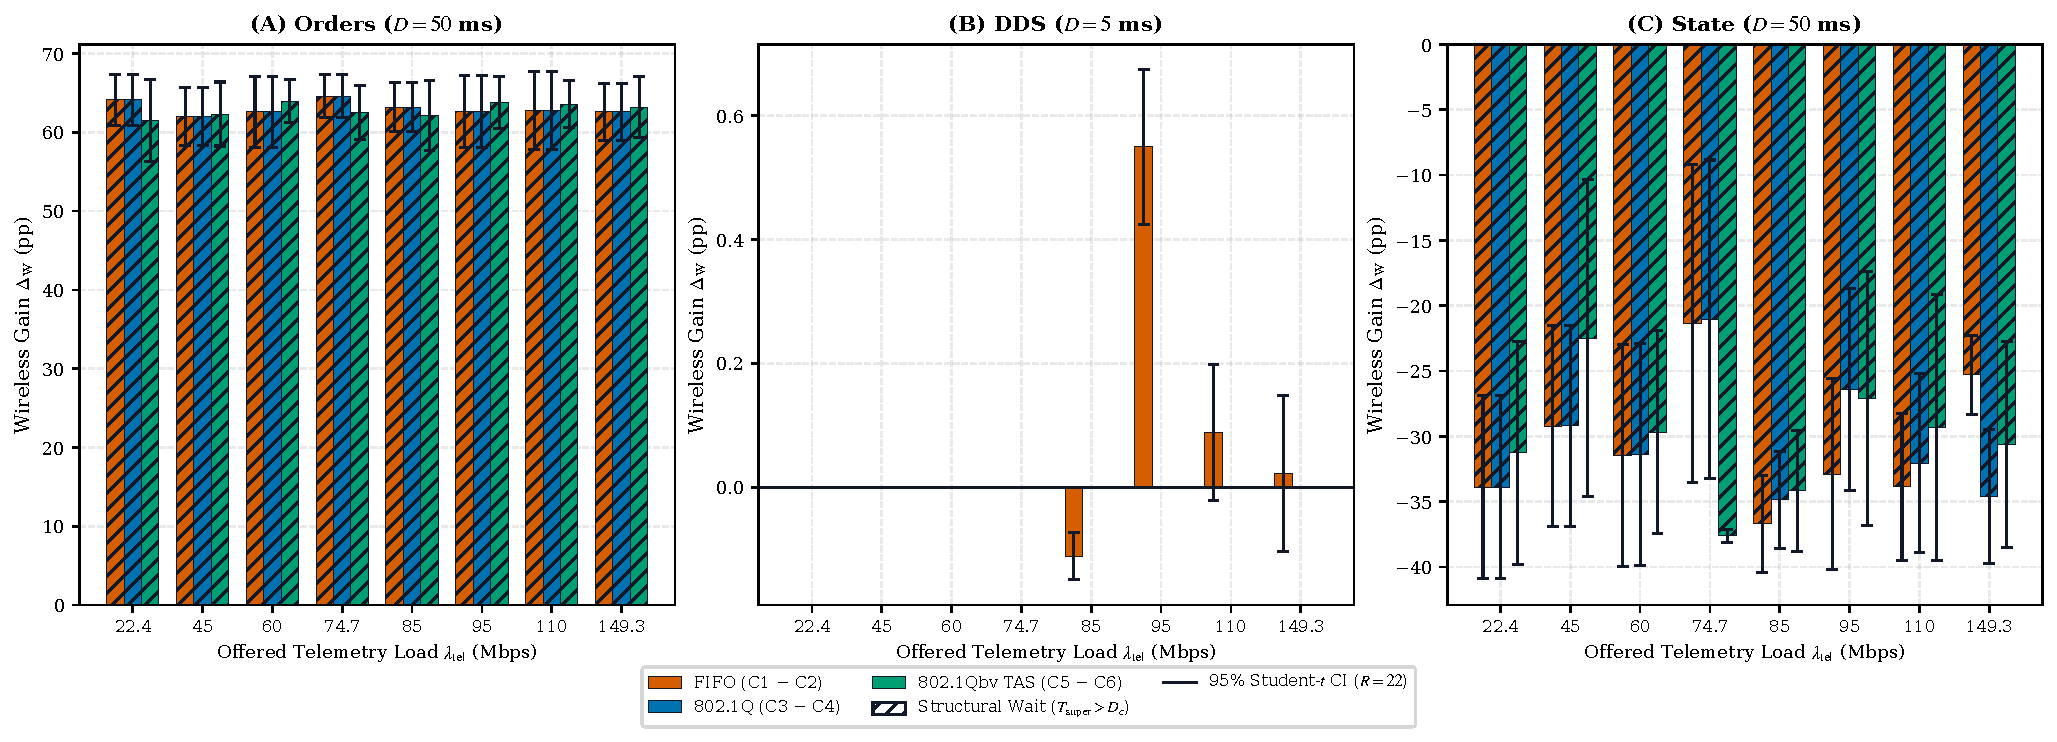
\includegraphics[width=0.95\textwidth]{images/pdf/fig_unpooled_n80.pdf}
\caption{Unpooled wireless TDMA upgrade contrast $\GainW = \MissB(\text{CSMA/CA}) - \MissB(\text{TDMA})$ at $(\Namr=80,\; \qty{12}{\mbps})$ stratified by wired switch discipline across all eight telemetry loads at uniform confirmatory depth ($R=22$): (A)~downlink Orders ($D=\qty{50}{\milli\second}$); (B)~inter-station DDS ($D=\qty{5}{\milli\second}$); (C)~uplink State ($D=\qty{50}{\milli\second}$). Error bars indicate 95\% Student-$t$ confidence intervals ($df=21$); hatched bars mark $\Tsuper > D_c$. Downlink Orders and DDS plot uniform $\MissB$ contrasts across all eight loads; continuous Watchdog $\MissA$ outcomes appear in \Cref{tab:aggregate_performance,tab:selected_points,tab:dual_stress_matrix,tab:conformance_summary}.}
\label{fig:unpooled_n80}
\end{figure}

\paragraph{Isolated Wireless Upgrade: AP Block Spillover at $\Namr=40$ vs.\ Contention Rescue at $\Namr=80$.}
At \qty{54}{\mbps} PHY ($\rho_{\mathrm{air,CSMA}} \le \qty{36.7}{\percent}$, $\rho_{\mathrm{air,sched}} \le \qty{28.6}{\percent}$), both CSMA/CA and Scheduled TDMA achieve $\MissB = \MissA = \qty{0.00}{\percent}$ on Orders and State below wired saturation (\Cref{fig:isolated_upgrades}B). At \qty{12}{\mbps} PHY, two distinct wireless failure mechanisms emerge as fleet size scales (\Cref{fig:isolated_upgrades}B, \Cref{fig:unpooled_n80}).

At moderate wireless load ($\Namr=40$, \qty{12}{\mbps}; $\rho_{\mathrm{air,CSMA}} = \qty{47.6}{\percent}$), the CSMA/CA radio channel remains unsaturated: Cells~1, 3, and~5 maintain $\MissB(\qty{50}{\milli\second}) = \MissA = \qty{0.00}{\percent}$ across all eight loads on downlink Orders (dedicated \texttt{eth[1]}), while uplink State holds \qty{0.00}{\percent} across all eight loads in wired-isolated Cells~3 and~5 (and through \qty{85.0}{\mbps} in Cell~1, before FIFO switch overflow raises Cell~1 State misses to \qty{3.99}{\percent} at \qty{95.0}{\mbps} and \qty{42.34}{\percent} in $R=22$ \texttt{supp-maxR} / \qty{42.54}{\percent} in \texttt{core-R3} at \qty{149.3}{\mbps}). Under TDMA, $\Tsuper = \qty{42}{\milli\second} < \qty{50}{\milli\second}$ preserves \qty{0.00}{\percent} uplink State misses across all eight loads in wired-isolated Cells~4 and~6 ($p_{99} \le \qty{42.88}{\milli\second}$, and through \qty{85.0}{\mbps} in Cell~2 before FIFO switch drops raise State misses to \qty{42.49}{\percent} in $R=22$ \texttt{supp-maxR} / \qty{42.40}{\percent} in \texttt{core-R3} at \qty{149.3}{\mbps}), whereas downlink Orders bursts spilling across the $K=10$ AP slot limit yield $\MissB = \qtyrange{4.15}{5.05}{\percent}$ (\qty{4.68}{\percent} 8-load mean) in Cells~2/4 and \qtyrange{4.53}{5.55}{\percent} (\qty{5.10}{\percent} mean) in Cell~6 (Watchdog $\MissA = \qty{6.86}{\percent}$ in Cells~2/4 and \qty{7.47}{\percent} in Cell~6; mean $\MissB$ contrast $\GainW = \qty{-4.68}{\pp}$ in Cells~2/4, \qty{-4.82}{\pp} across all three wired pairs), closely matching the $M/D^{10}/1$ analytical expectation (\qty{4.59}{\percent} $\MissB$, \qty{6.70}{\percent} $\MissA$).

At wireless contention saturation ($\Namr=80$, \qty{12}{\mbps}; $\rho_{\mathrm{air,CSMA}} = \qty{95.2}{\percent}$), CSMA/CA collapses on the single AP transmitter: AP buffer overflow drops (\qtyrange{10.40}{23.84}{\percent}) and severe contention backoff drive downlink Orders $\MissB(\qty{50}{\milli\second})$ to \qtyrange{93.57}{96.47}{\percent} (\qty{95.98}{\percent} $\MissB$ / \qty{96.30}{\percent} $\MissA$ in Cells~1/3 at $\ltel=\qty{22.4}{\mbps}$). Scheduled TDMA eliminates all AP drops ($\ploss = \qty{0.00}{\percent}$) and cuts Orders $\MissB$ to \qtyrange{31.55}{32.64}{\percent} ($\GainW = \qty{+64.09}{\pp}$ at \qty{22.4}{\mbps}; \qty{+63.07}{\pp} 8-load mean in Cells~1$\to$2 and~3$\to$4, \qty{+63.00}{\pp} across all three wired pairs; under Watchdog $\MissA$, $\qty{95.27}{\percent} \to \qty{39.12}{\percent}$, $\GainW = \qty{+56.15}{\pp}$ in Cells~1/3$\to$2/4, \Cref{fig:unpooled_n80}A), closely matching the three-part $M/D^{39}/1$ prediction (\qty{31.98}{\percent} $\MissB$, \qty{39.00}{\percent} $\MissA$). On the uplink, however, $\Tsuper = \qty{90}{\milli\second} > \qty{50}{\milli\second}$ raises State $\MissB$ at $\ltel=\qty{22.4}{\mbps}$ from \qty{6.03}{\percent} (Cells~1/3) to \qty{39.91}{\percent} (Cells~2/4, $\GainW = \qty{-33.88}{\pp}$, \Cref{fig:unpooled_n80}C).

\begin{table}[!tb]
\centering
\footnotesize
\setlength{\tabcolsep}{3.8pt}
\caption{Tick-quantized deadline miss spectrum $\MissB(D)$ (\%) across all seven evaluated thresholds $D \in \{1, 2, 5, 10, 20, 50, 100\}\,\text{ms}$ on the balanced 40-point \texttt{core-R3} pool ($\blacksquare$ marks nominal class budget $D_c$).}
\label{tab:deadline_spectrum}
\begin{tabular}{l l r r r r r r r r}
\toprule
\textbf{Class ($D_c$)} & \textbf{Cell Group} & \textbf{\qty{1}{\milli\second}} & \textbf{\qty{2}{\milli\second}} & \textbf{\qty{5}{\milli\second}} & \textbf{\qty{10}{\milli\second}} & \textbf{\qty{20}{\milli\second}} & \textbf{\qty{50}{\milli\second}} & \textbf{\qty{100}{\milli\second}} & \textbf{$\ploss$ (\%)} \\
\midrule
DDS & C1 (FIFO+CSMA) & 37.82 & 34.16 & $\blacksquare\,\mathbf{24.30}$ & 13.78 & 13.78 & 13.78 & 13.78 & 13.78 \\
(\qty{5}{\milli\second}) & C2 (FIFO+TDMA) & 37.78 & 34.12 & $\blacksquare\,\mathbf{24.26}$ & 13.76 & 13.76 & 13.76 & 13.76 & 13.76 \\
 & C3 to C6 (802.1Q / TAS) & \textbf{0.00} & \textbf{0.00} & $\blacksquare\,\mathbf{0.00}$ & \textbf{0.00} & \textbf{0.00} & \textbf{0.00} & \textbf{0.00} & \textbf{0.00} \\
\midrule
State & C1 (FIFO + CSMA) & 42.80 & 38.49 & 27.37 & 13.78 & 12.34 & $\blacksquare\,\mathbf{11.82}$ & 11.66 & 11.45 \\
(\qty{50}{\milli\second}) & C2 (FIFO + TDMA) & 75.54 & 71.37 & 60.12 & 44.41 & 29.15 & $\blacksquare\,\mathbf{15.55}$ & 11.51 & 11.51 \\
 & C3 (802.1Q + CSMA) & 4.86 & 3.74 & 2.31 & 1.41 & 0.82 & $\blacksquare\,\mathbf{0.39}$ & 0.23 & 0.01 \\
 & C4 (802.1Q + TDMA) & 56.64 & 51.00 & 38.89 & 27.76 & 16.47 & $\blacksquare\,\mathbf{3.99}$ & \textbf{0.00} & \textbf{0.00} \\
 & C5 (TAS + CSMA) & 6.51 & 3.93 & 2.36 & 1.43 & 0.83 & $\blacksquare\,\mathbf{0.42}$ & 0.27 & 0.01 \\
 & C6 (TAS + TDMA) & 58.88 & 52.93 & 39.98 & 28.31 & 16.67 & $\blacksquare\,\mathbf{4.03}$ & \textbf{0.00} & \textbf{0.00} \\
\midrule
Orders & C1 / C3 (CSMA) & 10.14 & 9.91 & 9.82 & 9.77 & 9.67 & $\blacksquare\,\mathbf{9.40}$ & 8.81 & 1.02 \\
(\qty{50}{\milli\second}) & C5 (TAS + CSMA) & 11.44 & 10.11 & 9.86 & 9.81 & 9.74 & $\blacksquare\,\mathbf{9.53}$ & 9.07 & 0.96 \\
 & C2 / C4 (TDMA) & 51.65 & 46.72 & 36.55 & 26.46 & 15.34 & $\blacksquare\,\mathbf{3.64}$ & 0.09 & \textbf{0.00} \\
 & C6 (TAS + TDMA) & 53.73 & 48.61 & 37.91 & 27.52 & 15.83 & $\blacksquare\,\mathbf{3.75}$ & 0.10 & \textbf{0.00} \\
\midrule
Telemetry & C1 / C2 (FIFO) & 37.93 & 33.94 & 22.68 & 10.13 & 10.13 & 10.13 & $\blacksquare\,\mathbf{10.13}$ & 10.13 \\
(\qty{100}{\milli\second}) & C3 / C4 (802.1Q) & 15.14 & 12.06 & 10.72 & 10.72 & 10.72 & 10.72 & $\blacksquare\,\mathbf{10.72}$ & 10.72 \\
 & C5 / C6 (802.1Qbv TAS) & 54.72 & 51.26 & 41.20 & 40.70 & 40.70 & 40.70 & $\blacksquare\,\mathbf{40.70}$ & 40.70 \\
\bottomrule
\end{tabular}
\end{table}

\paragraph{Seven-Deadline Spectrum and Sub-Superframe Crossover.}
Evaluating $\MissB(D)$ across all seven thresholds in \Cref{tab:deadline_spectrum} reveals three structural regimes: (1)~for wired-only FIFO flows (DDS and Telemetry in Cells~1/2), $\MissB(D)$ drops across $D \in \{1, 2, 5\}\,\text{ms}$ and plateaus to an exact constant equal to $\ploss$ for all $D \ge \qty{10}{\milli\second}$ (\qtyrange{13.76}{13.78}{\percent} DDS, \qty{10.13}{\percent} Telemetry), confirming the \qty{9.41}{\milli\second} FIFO drain ceiling in \Cref{eq:fifo_drain}; (2)~for tighter sub-superframe teleoperation deadlines ($D \le \qty{20}{\milli\second}$), CSMA/CA outperforms single-slot TDMA on both Orders (\qty{9.67}{\percent} vs.\ \qty{15.34}{\percent} at \qty{20}{\milli\second}) and State (\qty{0.82}{\percent} vs.\ \qty{16.47}{\percent}) because a single slot per superframe cannot guarantee sub-\qty{20}{\milli\second} phase latency; and (3)~at $D = \qty{100}{\milli\second} > \Tsuper = \qty{90}{\milli\second}$, Cells~4 and 6 achieve \qty{0.00}{\percent} State misses across all $40$ \texttt{core-R3} points ($\ploss = \qty{0.00}{\percent}$), whereas CSMA/CA (Cells~3/5) retains \qtyrange{0.23}{0.27}{\percent} misses from multi-second backoff stalls.

% =============================================================================
\subsection{RQ-(ii): Cross-Domain Masking and Negative Interaction}
\label{sec:rq2}

Companion-domain congestion caps single-domain upgrades whenever end-to-end deadlines depend on an unupgraded bottleneck, while adding deterministic TDMA phase wait in series with a congested FIFO switch induces a genuine negative cross-domain interaction on delivered State packets.

\begin{table}[!tb]
\centering
\footnotesize
\setlength{\tabcolsep}{2.6pt}
\caption{Three-domain delivered delay decomposition ($\tau_{\mathrm{wireless}}, \tau_{\mathrm{switch}}, \tau_{\mathrm{wire}}$ in \si{\milli\second}, packet-weighted per scenario and averaged equally across the 80 operating points) and exact per-cell unavailability ledger across all \num{6924} paired runs of \texttt{supp-maxR} (two-cell rows list per-cell counts).}
\label{tab:domain_delay_decomp}
\begin{tabular}{@{}l l r r r r r r r@{}}
\toprule
\textbf{Class} & \textbf{Cells} & \textbf{$\tau_{\mathrm{wireless}}$} & \textbf{$\tau_{\mathrm{switch}}$} & \textbf{$\tau_{\mathrm{wire}}$} & \textbf{$\ploss$ (\%)} & \begin{tabular}[c]{@{}r@{}}\textbf{Queue}\\(\textbf{$n_{\mathrm{drop,Q}}$/cell})\end{tabular} & \begin{tabular}[c]{@{}r@{}}\textbf{Retry}\\(\textbf{$n_{\mathrm{drop,R}}$/cell})\end{tabular} & \begin{tabular}[c]{@{}r@{}}\textbf{In-Fl.}\\(\textbf{/cell})\end{tabular} \\
\midrule
DDS & C1 (FIFO+CSMA) & 0.000 & 3.262 & 0.055 & 9.58 & \num{2493047} & 0 & 0 \\
 & C2 (FIFO+TDMA) & 0.000 & 3.262 & 0.055 & 9.58 & \num{2491927} & 0 & 0 \\
 & C3 / C4 (802.1Q) & 0.000 & 0.047 & 0.058 & \textbf{0.00} & 0 & 0 & 0 \\
 & C5 / C6 (TAS) & 0.000 & 0.339 & 0.058 & \textbf{0.00} & 0 & 0 & 0 \\
\midrule
State & C1 (FIFO+CSMA) & 11.591 & 3.239 & 0.169 & 8.01 & \num{2158618} & \num{26870} & \num{49288} \\
 & C2 (FIFO+TDMA) & 13.031 & 3.241 & 0.169 & 8.01 & \num{2199969} & 0 & 0 \\
 & C3 (802.1Q+CSMA) & 11.582 & 0.045 & 0.169 & 0.04 & \num{1123} & \num{26870} & \num{49238} \\
 & C4 (802.1Q+TDMA) & 13.031 & 0.045 & 0.169 & \textbf{0.00} & 0 & 0 & 0 \\
 & C5 (TAS+CSMA) & 13.385 & 0.415 & 0.169 & 0.04 & \num{1736} & \num{29535} & \num{53031} \\
 & C6 (TAS+TDMA) & 13.031 & 0.434 & 0.169 & \textbf{0.00} & 0 & 0 & 0 \\
\midrule
Orders & C1 / C3 (CSMA) & 24.507 & 0.000 & 0.105 & 1.58 & \num{609594} & 0 & \num{8664} \\
 & C5 (TAS+CSMA) & 24.844 & 0.561 & 0.105 & 1.63 & \num{629649} & 0 & \num{8696} \\
 & C2 / C4 (TDMA) & 12.479 & 0.000 & 0.105 & \textbf{0.00} & 0 & 0 & 43 \\
 & C6 (TAS+TDMA) & 12.364 & 0.564 & 0.105 & \textbf{0.00} & 0 & 0 & 44 \\
\midrule
Telemetry & C1 (FIFO+CSMA) & 0.000 & 3.245 & 0.249 & 7.06 & \num{55202050} & 0 & 0 \\
 & C2 (FIFO+TDMA) & 0.000 & 3.245 & 0.249 & 7.06 & \num{55191930} & 0 & 0 \\
 & C3 (802.1Q+CSMA) & 0.000 & 0.878 & 0.249 & 7.48 & \num{58236905} & 0 & 0 \\
 & C4 (802.1Q+TDMA) & 0.000 & 0.878 & 0.249 & 7.49 & \num{58318187} & 0 & 0 \\
 & C5 / C6 (TAS) & 0.000 & 3.947 & 0.247 & 37.18 & \num{216275202} & 0 & 0 \\
\bottomrule
\end{tabular}
\end{table}

\begin{figure}[!tb]
\centering
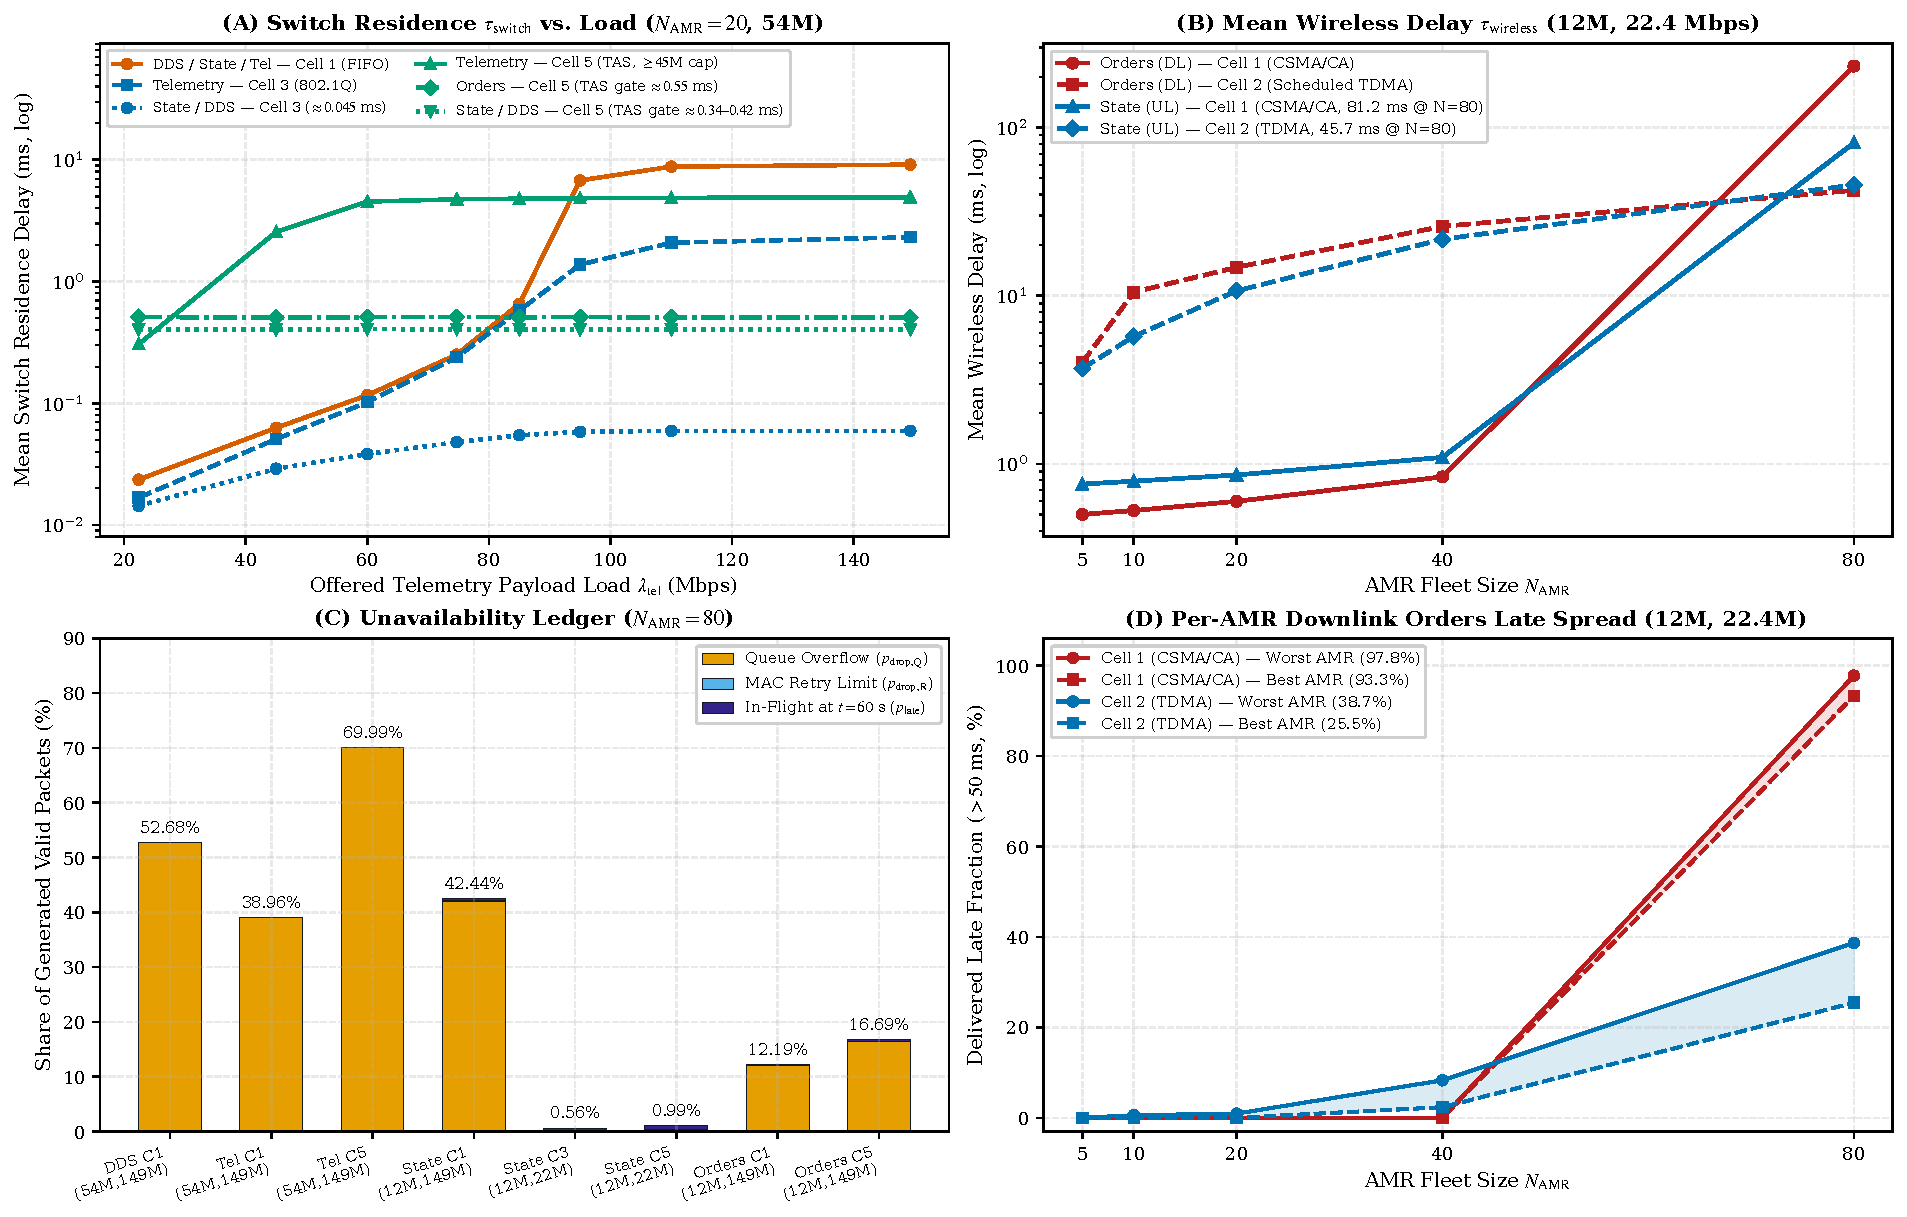
\includegraphics[width=0.95\textwidth]{images/pdf/fig_domain_drops.pdf}
\caption{Three-domain delay decomposition and $\Namr=80$ unavailability breakdown: (A)~wired switch residence $\tau_{\mathrm{switch}}$ vs.\ $\ltel$ ($\Namr=20,\; \qty{54}{\mbps}$); (B)~mean wireless delay $\tau_{\mathrm{wireless}}$ vs.\ $\Namr$ at $(\qty{12}{\mbps},\; \qty{22.4}{\mbps})$; (C)~unavailability decomposition ($p_{\mathrm{drop,Q}}, p_{\mathrm{drop,R}}, p_{\mathrm{late}}$) across $\Namr=80$ operating points; (D)~per-AMR downlink Orders late-delivery spread at $(\qty{12}{\mbps},\; \qty{22.4}{\mbps})$.}
\label{fig:domain_drops}
\end{figure}

\paragraph{Domain Delay and Drop Decomposition.}
Using the AP bridge timestamp $t_{\mathrm{ap}}$ and switch ingress/egress queue timestamps $(t_{\mathrm{sw,arr}}, t_{\mathrm{sw,dep}})$ (\Cref{fig:topology}), every delivered packet's end-to-end latency is partitioned exactly into $\tau_{\mathrm{e2e}} = \tau_{\mathrm{wireless}} + \tau_{\mathrm{switch}} + \tau_{\mathrm{wire}}$. \Cref{tab:domain_delay_decomp} and \Cref{fig:domain_drops,fig:ecdf_n80} show that: (1)~on \texttt{eth[0]}, 802.1Q (Cells~3/4) collapses mean switch residence $\tau_{\mathrm{switch}}$ for DDS and State from \qtyrange{3.24}{3.26}{\milli\second} (FIFO, peaking at \qty{9.11}{\milli\second} under saturation) to \qtyrange{0.045}{0.047}{\milli\second}, while TAS (Cells~5/6) introduces a deterministic \qtyrange{0.34}{0.56}{\milli\second} gate wait; (2)~in wireless CSMA/CA cells (Cells~1, 3, 5), downlink Orders suffer zero MAC retry drops ($n_{\mathrm{drop,R}} = 0$) because all Orders loss occurs via AP pending-queue overflow ($n_{\mathrm{drop,Q}} = \num{609594}$ packets per cell in Cells~1/3 and \num{629649} in Cell~5 at the 100-packet AP buffer cap, \Cref{fig:domain_drops}C), whereas TDMA Cells~2, 4, and~6 incur zero physical drops on downlink Orders and the wireless MAC ($0$ Orders queue drops and $0$ radio retry drops across all \num{3462} TDMA runs, leaving only $130$ terminal in-flight Orders frames across all three TDMA cells: $43$, $43$, and $44$, pooled ratio $3.36 \times 10^{-6}$ or \qty{0.00034}{\percent}; note that Cell~2 still incurs wired FIFO switch drops on \texttt{eth[0]} for State and DDS); and (3)~at $(\Namr=80,\; \qty{12}{\mbps},\; \qty{22.4}{\mbps})$, CSMA/CA penalizes every AMR uniformly on the downlink (\qtyrange{93.30}{97.75}{\percent} late delivered Orders in Cells~1/3, \qtyrange{91.15}{95.77}{\percent} in Cell~5, \Cref{fig:domain_drops}D and \Cref{fig:ecdf_n80}C), whereas Scheduled TDMA bounds per-AMR late Orders to \qtyrange{25.45}{38.65}{\percent} in Cells~2/4 (\qtyrange{25.99}{39.22}{\percent} in Cell~6).

\begin{figure}[!tb]
\centering
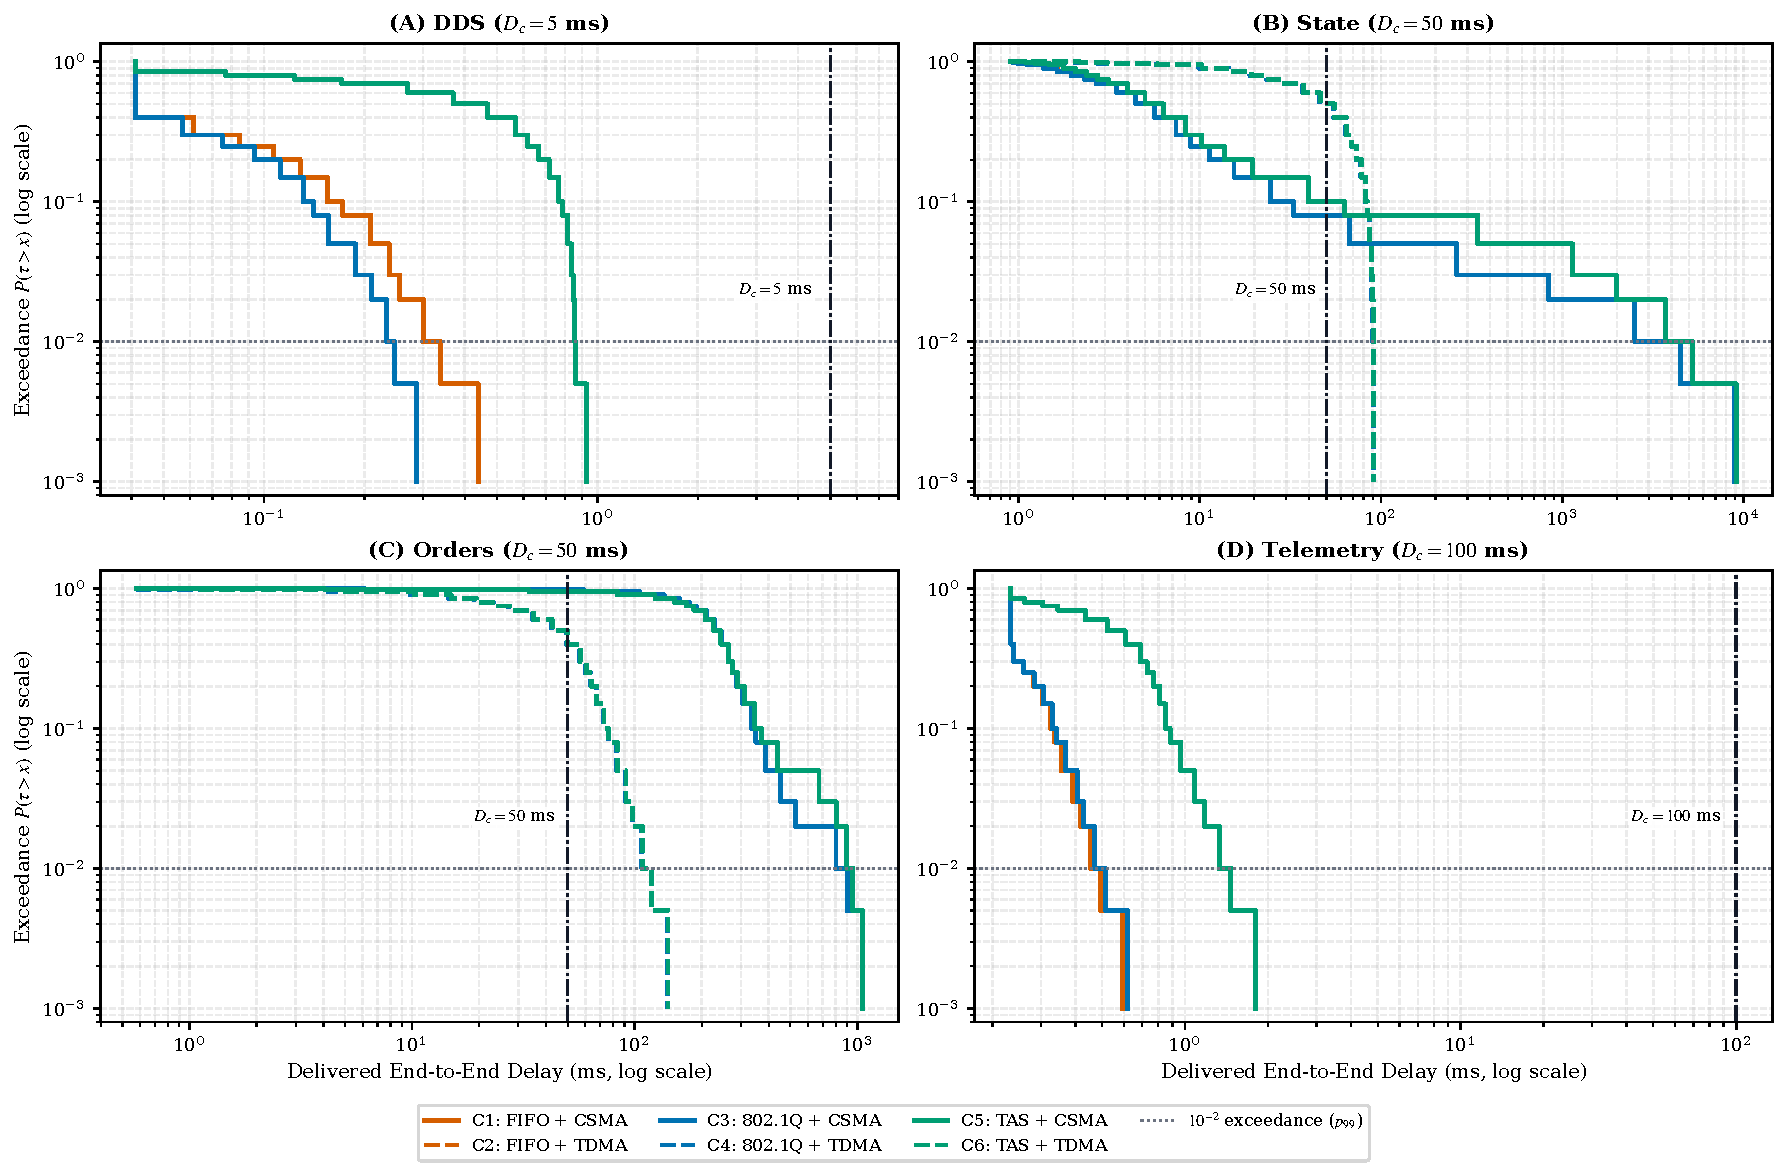
\includegraphics[width=0.94\textwidth]{images/pdf/fig_ecdf_n80.pdf}
\caption{Right-continuous step complementary cumulative distribution functions (CCDF, $P(\tau > x)$ on log-log axes across the 24 empirical quantile knots in $q \in [0.0, 0.999]$, where all $24/24$ curves satisfy $n_{\mathrm{deliv,valid}} \ge \num{410076} \ge 10^5$ for $p_{99.9}$ adequacy) for all six cells at $(\Namr=80,\; \qty{12}{\mbps},\; \ltel=\qty{22.4}{\mbps},\; R=22)$: (A)~DDS ($D_c=\qty{5}{\milli\second}$); (B)~uplink State ($D_c=\qty{50}{\milli\second}$); (C)~downlink Orders ($D_c=\qty{50}{\milli\second}$); (D)~Telemetry ($D_c=\qty{100}{\milli\second}$).}
\label{fig:ecdf_n80}
\end{figure}

\begin{figure}[!tb]
\centering
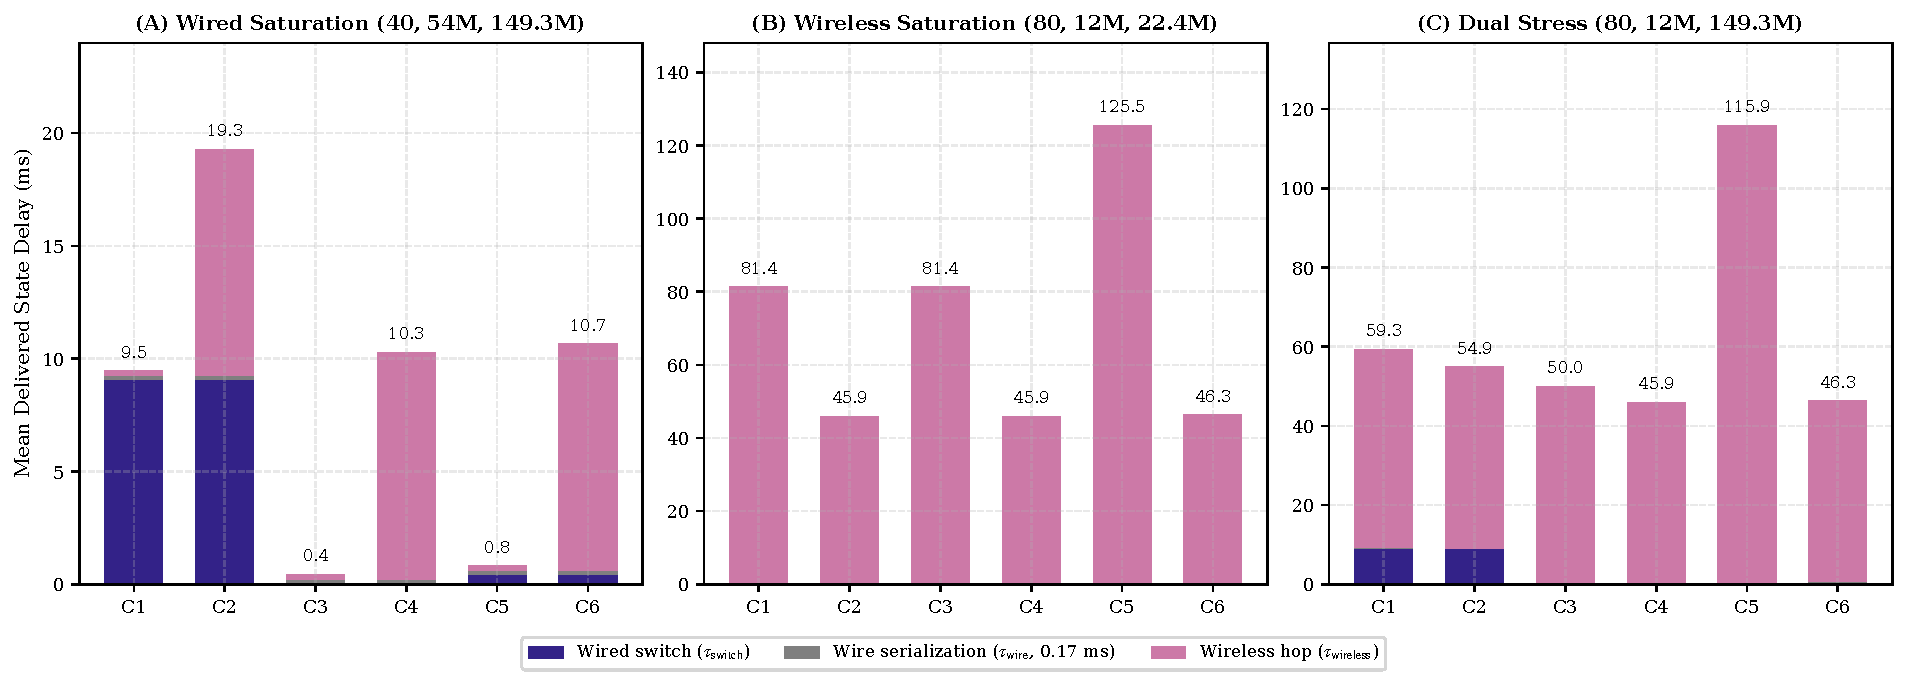
\includegraphics[width=0.95\textwidth]{images/pdf/fig_domain_bars.pdf}
\caption{Mean delivered State delay partitioned by domain across all six cells ($C_1$ to $C_6$) under the three benchmark regimes: (A)~wired saturation $(\Namr=40,\; \qty{54}{\mbps},\; \qty{149.3}{\mbps})$; (B)~wireless saturation $(\Namr=80,\; \qty{12}{\mbps},\; \qty{22.4}{\mbps})$; (C)~simultaneous dual-domain stress $(\Namr=80,\; \qty{12}{\mbps},\; \qty{149.3}{\mbps})$.}
\label{fig:domain_bars}
\end{figure}

\begin{table}[!tb]
\centering
\scriptsize
\setlength{\tabcolsep}{1.8pt}
\caption{Three-point cross-domain benchmark decomposed into queue drops, MAC retry drops, delivered late arrivals ($\MissB - \ploss - p_{\mathrm{late}}$), terminal in-flight packets ($p_{\mathrm{late}}$), and latency quantiles ($p_{50}, p_{99}$ in \si{\milli\second}) from \texttt{supp-maxR} (all three benchmarks at $R=22$). Multi-cell rows list slash-separated values in strict left-to-right cell order; KILL-class rows list nominal $\MissB$ above (or before) Watchdog-enforced $\MissA$ in parentheses (Late and In-Fl.\ reflect $\MissB$, whereas under Watchdog TTL all non-dropped $\MissA$ failures become Watchdog TTL discards).}
\label{tab:selected_points}
\begin{tabular}{@{}l l l r r r r r r r r@{}}
\toprule
\textbf{Scenario ($R$)} & \textbf{Class} & \textbf{Cell} & \textbf{$\MissB$} & \textbf{Queue} & \textbf{Retry} & \textbf{Late} & \textbf{In-Fl.} & \textbf{$\tau_{\mathrm{wl}}$} & \textbf{$\tau_{\mathrm{sw}}$} & \textbf{$p_{50} / p_{99}$} \\
 & & & \textbf{($\MissA$)} & & & & & & & \textbf{(ms)} \\
\midrule
Wired Stress & DDS & C1 / C2 & \begin{tabular}[t]{@{}r@{}}71.6/71.6\\(100.0)\end{tabular} & 51.6/51.6 & 0.00 & 20.0/20.0 & 0.00 & 0.00 & 9.11 & 9.19 / 9.52 \\
$(40,54\text{M},$ & & C3 to C6 & \textbf{0.00} (0.00) & \textbf{0.00} & 0.00 & \textbf{0.00} & 0.00 & 0.00 & $\le 0.34$ & $\le 0.40 / 0.96$ \\
$149.3\text{M},R{=}22)$ & State & C1 & 42.80 & 42.80 & 0.00 & 0.00 & 0.00 & 0.22 & 9.07 & 9.46 / 9.93 \\
 & & C2 & 42.75 & 42.75 & 0.00 & 0.00 & 0.00 & 10.04 & 9.07 & 19.28 / 29.10 \\
 & & C3 / C5 & \textbf{0.00} & \textbf{0.00} & 0.00 & \textbf{0.00} & 0.00 & 0.22 & $\le 0.42$ & $\le 0.81 / 1.58$ \\
 & & C4 / C6 & \textbf{0.00} & \textbf{0.00} & 0.00 & \textbf{0.00} & 0.00 & 10.04 & $\le 0.45$ & \begin{tabular}[t]{@{}r@{}}$\le 10.66$ /\\20.53\end{tabular} \\
\midrule
Wireless Stress & State & C1 / C3 & 6.03 & 0.02 & 0.20 & 5.47 & 0.34 & 81.17 & $\le 0.02$ & 4.44 / 2516.5 \\
$(80,\; 12\text{M},$ & & C5 & 9.26 & 0.04 & 0.35 & 8.26 & 0.61 & 124.90 & 0.40 & 4.99 / 3698.2 \\
$22.4\text{M},\; R{=}22)$ & & C2/C4/C6 & 39.9/40.5 & \textbf{0.00} & \textbf{0.00} & 39.9/40.5 & \textbf{0.00} & 45.74 & $\le 0.41$ & \begin{tabular}[t]{@{}r@{}}45.9/46.3 /\\90.4\end{tabular} \\
 & Orders & C1 / C3 & 95.98 (96.30) & 12.58 & 0.00 & 83.20 & 0.20 & 232.44 & 0.00 & 227.7 / 803.0 \\
 & & C5 & 93.99 (94.41) & 14.93 & 0.00 & 78.88 & 0.18 & 235.92 & 0.76 & 226.2 / 894.5 \\
 & & C2/C4/C6 & \begin{tabular}[t]{@{}r@{}}\textbf{31.9/32.5}\\(39.2/39.8)\end{tabular} & \textbf{0.00} & \textbf{0.00} & 31.9/32.5 & \textbf{0.00} & 42.4/42.1 & $\le 0.78$ & \begin{tabular}[t]{@{}r@{}}42.1/42.6 /\\108.0\end{tabular} \\
\midrule
Dual Stress & DDS & C1 / C2 & \begin{tabular}[t]{@{}r@{}}72.4/72.3\\(100.0)\end{tabular} & 52.9/52.9 & 0.00 & 19.4/19.5 & 0.00 & 0.00 & 9.06 & 9.13 / 9.49 \\
$(80,\; 12\text{M},$ & & C3 to C6 & \textbf{0.00} (0.00) & \textbf{0.00} & 0.00 & \textbf{0.00} & 0.00 & 0.00 & $\le 0.34$ & $\le 0.40 / 0.96$ \\
$149.3\text{M},\; R{=}22)$ & State & C1 & 45.70 & 41.98 & 0.17 & 3.27 & 0.29 & 50.08 & 9.01 & 13.39 / 1328.3 \\
 & & C2 & \textbf{70.98} & 42.17 & \textbf{0.00} & \textbf{28.82} & \textbf{0.00} & 45.73 & 8.99 & \textbf{54.89} / 98.95 \\
 & & C3 & 5.40 & 0.01 & 0.17 & 4.94 & 0.29 & 49.77 & 0.06 & 4.44 / 1293.4 \\
 & & C5 & 9.89 & 0.01 & 0.36 & 8.85 & 0.67 & 115.32 & 0.40 & 5.12 / 3190.5 \\
 & & C4 / C6 & 39.98/40.52 & \textbf{0.00} & \textbf{0.00} & 40.0/40.5 & \textbf{0.00} & 45.72 & $\le 0.41$ & \begin{tabular}[t]{@{}r@{}}46.0/46.3 /\\90.39\end{tabular} \\
 & Orders & C1/C3/C5 & \begin{tabular}[t]{@{}r@{}}94.5/95.6\\(94.9/95.9)\end{tabular} & 12.0/16.4 & 0.00 & 82.3/78.9 & 0.21/0.26 & 228.4/245.8 & $\le 0.76$ & \begin{tabular}[t]{@{}r@{}}228.5/231.2 /\\775.8/902.8\end{tabular} \\
 & & C2/C4/C6 & \begin{tabular}[t]{@{}r@{}}\textbf{31.9/32.5}\\(39.2/39.7)\end{tabular} & \textbf{0.00} & \textbf{0.00} & 31.9/32.5 & \textbf{0.00} & 42.3/41.9 & $\le 0.79$ & \begin{tabular}[t]{@{}r@{}}42.2/42.6 /\\104.5\end{tabular} \\
\bottomrule
\end{tabular}
\end{table}

\paragraph{Cell~5 vs.\ Cell~3 Wireless Tail Divergence Under Metastable CSMA/CA.}
At first glance, \Cref{tab:selected_points} exhibits a striking divergence between Cell~3 (802.1Q+CSMA) and Cell~5 (TAS+CSMA) on uplink State at $(\Namr=80,\; \qty{12}{\mbps})$: mean $\tau_{\mathrm{wl}}$ rises from \qty{81.17}{\milli\second} to \qty{124.90}{\milli\second} at \qty{22.4}{\mbps} and from \qty{49.8}{\milli\second} to \qty{115.3}{\milli\second} at \qty{149.3}{\mbps}, even though \texttt{eth[0]} TAS gating lies downstream of the radio link in an open-loop UDP network. Across all $176$ paired CSMA runs at $(\Namr=80,\; \qty{12}{\mbps})$ ($8\text{ loads} \times 22\text{ seeds}$), however, Cells~1 and~3 produce bit-identical wireless MAC retry drops ($176/176$) and AP Orders drops ($176/176$), whereas Cell~5 delays downlink Orders on \texttt{eth[1]} by \qtyrange{0.5}{0.76}{\milli\second} through the cyclic TC3 gate. That sub-millisecond early AP timing shift desynchronizes the shared \texttt{rng-0} CSMA backoff trajectory on the metastable \qty{95.2}{\percent} utilization channel while preserving rank correlation from shared \texttt{rng-2} AMR coordinates (Spearman $\rho = 0.722$ on State $\MissB$, $0.808$ on Orders queue drops). Paired Wilcoxon signed-rank tests across all $176$ pairs confirm \emph{zero systematic degradation} in Cell~5: median paired State $\MissB$ difference is \qty{+0.00}{\pp} ($\text{C5} > \text{C3}$ on $88/176 = \qty{50.0}{\percent}$, Wilcoxon $p = 0.486$, sign $p = 1.000$), median $\tau_{\mathrm{wl}}$ difference is \qty{+0.03}{\milli\second} ($p = 0.661$), median $p_{99}$ difference is \qty{-0.13}{\milli\second} ($p = 0.852$), and extreme runaway collapses ($\ge \qty{50}{\percent}$ State misses) match identically ($13/176 = \qty{7.39}{\percent}$ in each cell, Fisher exact $p = 1.000$; $\ge \qty{10}{\percent}$ stalls: $29/176$ vs.\ $31/176$, $p = 0.887$). Stratifying each $22$-seed slice into three State $\MissB$ regimes (normal $< \qty{10}{\percent}$ / intermediate \qtyrange{10}{50}{\percent} / collapsed $\ge \qty{50}{\percent}$; \Cref{sec:micro_diagnostics}, \Cref{tab:collapse_incidence}), the slice-level gaps in \Cref{tab:selected_points} reflect two extra intermediate-stall seeds in Cell~5 at \qty{22.4}{\mbps} (C3: \num{21}/0/1 vs.\ C5: \num{19}/2/1) and three extra intermediate seeds at \qty{149.3}{\mbps} (\num{20}/1/1 vs.\ \num{17}/4/1), which reverse completely at \qty{74.7}{\mbps} (C3: \num{16}/0/6, \qty{18.89}{\percent} vs.\ C5: \num{22}/0/0, \qty{2.87}{\percent}; \qty{-16.02}{\pp}, \Cref{fig:unpooled_n80}C). Furthermore, because all sources share \texttt{rng-1} (\Cref{sec:topology}), valid generation counts vary across the eight telemetry loads on $22/22$ seeds, generating eight correlated realizations over the $22$ fixed \texttt{rng-2} layouts (Cell~3 cross-load Spearman $\rho = 0.644$, with unfavorable layout $r=3$ stalling on $8/8$ loads in Cell~3 and $6/8$ in Cell~5). Away from metastability at $(\Namr=40,\; \qty{12}{\mbps})$, \qty{1}{\milli\second} TC3 pacing slightly de-bursts AP arrivals and reduces wireless Orders latency on $176/176$ runs (\qty{0.837}{\milli\second} $\to$ \qty{0.785}{\milli\second}, median \qty{-52}{\micro\second}, Wilcoxon $p = 1.24 \times 10^{-30}$).

\paragraph{Naive Additive Domain-Share Baseline and Negative Cross-Domain Interaction.}
To quantify where simple additive domain attribution succeeds or breaks down across $\Namr \in \{40, 80\}$ ($R=22$), \Cref{tab:hypothesis_test} evaluates a naive linear baseline constructed strictly from Cell~1 outputs without consulting upgraded cells. Directly attributing Cell~1 wireless retry drops ($p_{\mathrm{drop,wl}}^{(1)} = p_{\mathrm{drop,R}}^{(1)}$ for State and $\ploss^{(1)}$ for wireless-only Orders) versus wired/queue drops ($p_{\mathrm{drop,wd}}^{(1)} = p_{\mathrm{drop,Q}}^{(1)}$ for State, noting that \texttt{ExperimentCoordinator} records aggregate \texttt{n\_drop\_Q} combining \qtyrange{6.3}{42.0}{\percent} wired switch drops with \qtyrange{0.01}{0.04}{\percent} wireless AMR queue drops; and $\ploss^{(1)}$ for wired-only DDS), and weighting baseline non-drop misses ($\MissB^{(1)} - \ploss^{(1)}$) by Cell~1 packet-weighted delay shares $(s_{\tau,\mathrm{wd}}^{(1)}, s_{\tau,\mathrm{wl}}^{(1)})$ where $\tau_{\mathrm{wd}} = \tau_{\mathrm{switch}} + \tau_{\mathrm{wire}}$, yields the naive linear-share predictors
\begin{equation}
\widehat{\GainP} = p_{\mathrm{drop,wd}}^{(1)} + s_{\tau,\mathrm{wd}}^{(1)}\!\left(\MissB^{(1)} - \ploss^{(1)}\right), \qquad
\widehat{\GainW} = p_{\mathrm{drop,wl}}^{(1)} + s_{\tau,\mathrm{wl}}^{(1)}\!\left(\MissB^{(1)} - \ploss^{(1)}\right).
\label{eq:hyp_pred}
\end{equation}

\begin{table}[!tb]
\centering
\scriptsize
\setlength{\tabcolsep}{2.2pt}
\caption{Confirmatory $R=22$ naive additive domain-share baseline across $\Namr \in \{40, 80\}$ (\texttt{supp-maxR}): Cell~1 baseline miss rate ($\MissB^{(1)}$), Cell-1-only wired (\textbf{Wd}) and wireless (\textbf{Wl}) packet-weighted delay and drop shares ($s_{\tau}/s_L$, \%), naive linear predictors ($\widehat{\Delta}$, \Cref{eq:hyp_pred}), and observed single-pair gains ($\GainPpair$: C1$\to$C3; $\GainWpair$: C1$\to$C2, \si{\pp}). Rightmost percentages report observed/predicted ratios on non-trivial points; pure wired-overload rows where $\text{C3}=\qty{0.00}{\percent}$ equal $\widehat{\GainP}$ by algebraic identity.}
\label{tab:hypothesis_test}
\begin{tabular}{@{}l l r r r r r l@{}}
\toprule
\textbf{($\Namr$, PHY, $\ltel$)} & \textbf{Class} & \textbf{C1 (\%)} & \multicolumn{2}{c}{\textbf{Shares $s_{\tau}/s_L$ (\%)}} & \textbf{$\GainPpair$ (\si{\pp})} & \textbf{$\GainWpair$ (\si{\pp})} & \textbf{Outcome} \\
\cmidrule(lr){4-5}
 & & \textbf{$\MissB^{(1)}$} & \textbf{Wd} & \textbf{Wl} & \textbf{Pred / Obs} & \textbf{Pred / Obs} & \\
\midrule
40, 54M, 149.3M & DDS & 71.60 & 100 / 100 & 0 / 0 & 71.60 / +71.60 & 0.00 / $-$0.02 & Wired identity ($\text{C3}=0$) \\
 & State & 42.80 & 97.7 / 100 & 2.3 / 0 & 42.80 / +42.80 & 0.00 / +0.05 & Wired identity ($\text{C3}=0$) \\
80, 54M, 149.3M & DDS & 72.29 & 100 / 100 & 0 / 0 & 72.29 / +72.29 & 0.00 / $-$0.03 & Wired identity ($\text{C3}=0$) \\
 & State & 43.06 & 97.2 / 100 & 2.8 / 0 & 43.06 / +43.06 & 0.00 / \textbf{$-$3.13} & Pure interaction \\
\midrule
40, 12M, 22.4M & Orders & 0.00 & 11.2 / 0 & 88.8 / 0 & 0.00 / 0.00 & 0.00 / \textbf{$-$5.05} & Neg.\ (AP spill) \\
 & State & 0.00 & 14.6 / 0 & 85.4 / 0 & 0.00 / 0.00 & 0.00 / 0.00 & Zero baseline \\
80, 12M, 22.4M & Orders & 95.98 & 0.0 / 0 & 100 / 100 & 0.04 / 0.00 & 95.94 / \textbf{+64.09} & W: \qty{66.8}{\percent} \\
 & State & 6.03 & 0.2 / 10.2\textsuperscript{a} & 99.8 / 89.8 & 0.04 / 0.00 & 5.99 / \textbf{$-$33.88} & Neg.\ ($\Tsuper{>}D_c$) \\
\midrule
80, 12M, 95.0M & State & 19.76 & 5.8 / 92.3 & 94.2 / 7.7 & 7.06 / \textbf{+6.19} & 12.70 / \textbf{$-$32.87} & P: \qty{87.8}{\percent}; W neg. \\
80, 12M, 149.3M & DDS & 72.36 & 100 / 100 & 0 / 0 & 72.36 / +72.36 & 0.00 / +0.02 & Wired identity ($\text{C3}=0$) \\
 & Orders & 94.50 & 0.0 / 0 & 100 / 100 & 0.04 / 0.00 & 94.46 / \textbf{+62.61} & W: \qty{66.3}{\percent} \\
 & State & 45.70 & 15.5 / 99.6 & 84.5 / 0.4 & 42.54 / \textbf{+40.31} & 3.17 / \textbf{$-$25.28} & P: \qty{94.8}{\percent}; W neg. \\
\bottomrule
\end{tabular}
\par\vspace{2pt}
\raggedright\scriptsize
\textsuperscript{a}\,Artifact of pooling switch and wireless AMR MAC queue drops in \texttt{n\_drop\_Q}: on the uncongested \qty{22.4}{\mbps} wired trunk, all \qty{0.02}{\percent} queue drops occur in wireless AMR MAC queues.
\end{table}

Partitioning all $240$ critical class-scenario pairs ($80\text{ points} \times 3\text{ critical classes}$) clarifies the narrow empirical scope of linear attribution: $132/240$ pairs are exact all-zero baselines ($\text{C1}=\text{C2}=\text{C3}=0$), $26/240$ are zero-baseline TDMA penalties ($\text{C1}=0,\; \text{C2}>0$, comprising $24$ Orders slices at $\Namr \in \{10, 20, 40\},\; \qty{12}{\mbps}$ plus two single-packet \qty{0.0002}{\percent} State points), $66/240$ are pure wired-overload identities where $\text{C3}=\qty{0.00}{\percent}$ forces $\GainPpair = \widehat{\GainP}$, and $12/240$ are pure wireless bottlenecks ($\text{C1}\approx\text{C3}$, $s_{\tau,\mathrm{wl}}\ge \qty{99}{\percent}$, spanning $8$ Orders points and $\le \qty{74.7}{\mbps}$ State at $\Namr=80,\; \qty{12}{\mbps}$). Only $4/240$ pairs represent genuinely mixed dual-stress regimes, all on State at $(\Namr=80,\; \qty{12}{\mbps},\; \ltel \in \{85.0, 95.0, 110.0, 149.3\}\,\text{Mbps})$ (with $3$ points at $\ltel \ge \qty{95.0}{\mbps}$ carrying heavy wired drops). Across the archive, \Cref{eq:hyp_pred} records \num{0}/240 wired exceedances ($\GainPpair > \widehat{\GainP} + \qty{0.05}{\pp}$) and \num{21}/240 minor stochastic wireless exceedances ($\le \qty{1.40}{\pp}$ at exploratory $R=3$ slices and $\le \qty{0.61}{\pp}$ at $R=22$ above $\widehat{\GainW} \approx 0$, attributable to paired FIFO telemetry queue variation). On those non-trivial mixed State points, 802.1Q realizes \qty{87.8}{\percent} of $\widehat{\GainP}$ at \qty{95.0}{\mbps} ($\qty{+6.19}{\pp}\text{ vs.\ }\qty{7.06}{\pp}$) and \qty{94.8}{\percent} at \qty{149.3}{\mbps} ($\qty{+40.31}{\pp}\text{ vs.\ }\qty{42.54}{\pp}$); on the wireless upgrade, $\Namr=80,\; \qty{12}{\mbps}$ Orders captures \qtyrange{66.2}{67.1}{\percent} of $\widehat{\GainW}$ across all eight loads (\qty{+62.02}{\pp} to \qty{+64.59}{\pp} vs.\ $93.53\text{ to }\qty{96.23}{\pp}$), capped by the trailing \qty{90}{\milli\second} AP block.

Conversely, linear share weighting fails whenever deterministic TDMA scheduling reshapes the wireless delay distribution rather than scaling it. The cleanest unconfounded proof of negative cross-domain interaction appears at $(\Namr=80,\; \qty{54}{\mbps},\; \qty{149.3}{\mbps})$ (\Cref{tab:hypothesis_test}): here TDMA alone produces \qty{0.00}{\percent} State misses ($\Tsuper = \qty{48}{\milli\second} < \qty{50}{\milli\second}$; Cell~4 $p_{99}=\qty{47.79}{\milli\second}$) and wired FIFO alone produces \qty{0.00}{\percent} delivered late arrivals ($\tau_{\mathrm{FIFO,max}} = \qty{9.41}{\milli\second}$, only \qty{43.06}{\percent} buffer drops), yet combining TDMA with FIFO pushes $p_{99}$ to \qty{56.72}{\milli\second} ($p_{50} = \qty{33.24}{\milli\second}$) and induces a pure cross-domain late-arrival penalty of $\GainWpair = \qty{-3.13}{\pp}$ (\qty{43.06}{\percent} $\to$ \qty{46.19}{\percent}). At $(\Namr=80,\; \qty{12}{\mbps})$, by contrast, the raw \qty{-33.88}{\pp} penalty at \qty{22.4}{\mbps} reflects $\Tsuper = \qty{90}{\milli\second} > \qty{50}{\milli\second}$ directly (a large negative prediction error below $\widehat{\GainW} = \qty{+5.99}{\pp}$). Under joint saturation at \qty{149.3}{\mbps}, most of Cell~2's \qty{70.98}{\percent} State miss rate stems from those \qty{42.17}{\percent} FIFO drops plus the \qty{90}{\milli\second} cycle wait, while the genuine cross-domain interaction appears among \emph{delivered} State packets, whose late fraction rises by \qty{+9.92}{\pp} from \qty{39.91}{\percent} at \qty{22.4}{\mbps} to \qty{49.83}{\percent} at \qty{149.3}{\mbps} ($p_{50} = \qty{54.89}{\milli\second} > \qty{50}{\milli\second}$). Underlying collapse skewness, spatial capture, and TAS/TDMA phase alignment are examined in \Cref{sec:micro_diagnostics}.

% =============================================================================
\subsection{RQ-(iii): Dual-Domain Determinism and Operating-Envelope Screening}
\label{sec:rq3}

Coordinated deterministic scheduling in both domains (Cells~4 and~6) is required whenever offered telemetry on \texttt{eth[0]} exceeds \qtyrange{85}{95}{\mbps} \emph{and} wireless contention nears saturation ($\Namr=80$ at \qty{12}{\mbps}, $\rho_{\mathrm{air,CSMA}} = \qty{95.2}{\percent}$, $\rho_{\mathrm{air,sched}} = \qty{87.1}{\percent}$); under simultaneous saturation, however, zero physical loss in Cells~4 and~6 is necessary rather than sufficient because single-slot \qty{90}{\milli\second} TDMA superframes still miss a \qty{50}{\milli\second} State budget evaluated on the \qty{10}{\milli\second} tick grid (\qtyrange{40.0}{40.5}{\percent} State misses, \qtyrange{31.9}{32.5}{\percent} $\MissB$ / \qtyrange{39.2}{39.7}{\percent} Watchdog $\MissA$ on Orders), requiring \qty{54}{\mbps} PHY ($\Tsuper = \qty{48}{\milli\second}$) or multi-slot/multi-channel scheduling.

\begin{table}[!tb]
\centering
\scriptsize
\setlength{\tabcolsep}{2.2pt}
\caption{Numeric $3 \times 2$ dual-stress matrix at simultaneous wired and wireless saturation $(\Namr=80,\; \qty{12}{\mbps},\; \ltel=\qty{149.3}{\mbps},\; R=22)$, reporting nominal $\MissB$ (\%) (with Watchdog-enforced $\MissA$ (\%) in parentheses for KILL classes DDS and Orders) stacked above physical loss $\ploss$ (\%), alongside State $p_{99}$ tail latency (\si{\milli\second}).}
\label{tab:dual_stress_matrix}
\begin{tabular}{@{}l r r r r r r r r@{}}
\toprule
 & \multicolumn{4}{c}{\textbf{IEEE 802.11g CSMA/CA (Cells 1, 3, 5)}} & \multicolumn{4}{c}{\textbf{Scheduled TDMA (Cells 2, 4, 6)}} \\
\cmidrule(lr){2-5} \cmidrule(lr){6-9}
\textbf{Wired} & \textbf{DDS} & \textbf{Orders} & \textbf{State} & \textbf{State} & \textbf{DDS} & \textbf{Orders} & \textbf{State} & \textbf{State} \\
\textbf{Switch} & \textbf{$\MissB(\MissA)$} & \textbf{$\MissB(\MissA)$} & \textbf{$\MissB$} & \textbf{$p_{99}$} & \textbf{$\MissB(\MissA)$} & \textbf{$\MissB(\MissA)$} & \textbf{$\MissB$} & \textbf{$p_{99}$} \\
 & \textbf{/\,$\ploss$ (\%)} & \textbf{/\,$\ploss$ (\%)} & \textbf{/\,$\ploss$ (\%)} & \textbf{(ms)} & \textbf{/\,$\ploss$ (\%)} & \textbf{/\,$\ploss$ (\%)} & \textbf{/\,$\ploss$ (\%)} & \textbf{(ms)} \\
\midrule
FIFO & \begin{tabular}[t]{@{}r@{}}72.4 (100)\\/\,52.9\end{tabular} & \begin{tabular}[t]{@{}r@{}}94.5 (94.9)\\/\,12.0\end{tabular} & \begin{tabular}[t]{@{}r@{}}45.7\\/\,42.2\end{tabular} & 1328.3 & \begin{tabular}[t]{@{}r@{}}72.3 (100)\\/\,52.9\end{tabular} & \begin{tabular}[t]{@{}r@{}}31.9 (39.2)\\/\,\textbf{0.0}\end{tabular} & \begin{tabular}[t]{@{}r@{}}71.0\\/\,42.2\end{tabular} & 99.0 \\
(C1, C2) & & & & & & & & \\
\addlinespace[2pt]
802.1Q & \begin{tabular}[t]{@{}r@{}}\textbf{0.0} (0.0)\\/\,\textbf{0.0}\end{tabular} & \begin{tabular}[t]{@{}r@{}}94.5 (94.9)\\/\,12.0\end{tabular} & \begin{tabular}[t]{@{}r@{}}5.4\\/\,0.17\end{tabular} & 1293.4 & \begin{tabular}[t]{@{}r@{}}\textbf{0.0} (0.0)\\/\,\textbf{0.0}\end{tabular} & \begin{tabular}[t]{@{}r@{}}\textbf{31.9} (39.2)\\/\,\textbf{0.0}\end{tabular} & \begin{tabular}[t]{@{}r@{}}40.0\\/\,\textbf{0.0}\end{tabular} & \textbf{90.0} \\
(C3, C4) & & & & & & & & \\
\addlinespace[2pt]
802.1Qbv & \begin{tabular}[t]{@{}r@{}}\textbf{0.0} (0.0)\\/\,\textbf{0.0}\end{tabular} & \begin{tabular}[t]{@{}r@{}}95.6 (95.9)\\/\,16.4\end{tabular} & \begin{tabular}[t]{@{}r@{}}9.9\\/\,0.37\end{tabular} & 3190.5 & \begin{tabular}[t]{@{}r@{}}\textbf{0.0} (0.0)\\/\,\textbf{0.0}\end{tabular} & \begin{tabular}[t]{@{}r@{}}\textbf{32.5} (39.7)\\/\,\textbf{0.0}\end{tabular} & \begin{tabular}[t]{@{}r@{}}40.5\\/\,\textbf{0.0}\end{tabular} & \textbf{90.4} \\
(C5, C6) & & & & & & & & \\
\bottomrule
\end{tabular}
\end{table}

\paragraph{Simultaneous Dual-Domain Stress Matrix.}
\Cref{tab:dual_stress_matrix} presents the $3 \times 2$ numeric outcome matrix under simultaneous wired and wireless saturation $(\Namr=80,\; \qty{12}{\mbps},\; \ltel=\qty{149.3}{\mbps},\; R=22)$. All four single-domain or unupgraded configurations fail critically: Cell~1 collapses across all three critical classes (\qty{72.36}{\percent} $\MissB$ / \qty{100.0}{\percent} $\MissA$ DDS, \qty{94.50}{\percent} / \qty{94.88}{\percent} Orders, \qty{45.70}{\percent} State); wireless-only Cell~2 eliminates wireless loss but leaves DDS at \qty{72.33}{\percent} (\qty{100.0}{\percent} $\MissA$) and raises State misses to \qty{70.98}{\percent}; and wired-only Cells~3 and~5 restore DDS to \qty{0.00}{\percent} and eliminate wired State drops, but leave Orders collapsed (\qtyrange{94.50}{95.62}{\percent} $\MissB$ / \qtyrange{94.88}{95.93}{\percent} $\MissA$ with \qtyrange{11.99}{16.43}{\percent} AP buffer drops) and expose State to multi-second CSMA/CA tails ($p_{99} = \qty{1293.4}{\milli\second}$ in Cell~3, \qty{3190.5}{\milli\second} in Cell~5). Only the dual-domain cells (Cell~4: 802.1Q + TDMA; Cell~6: 802.1Qbv TAS + TDMA) achieve \qty{0.00}{\percent} physical packet loss ($\ploss = 0$) across all three critical classes simultaneously while bounding worst-case State $p_{99}$ latency to \qtyrange{90.0}{90.4}{\milli\second} (\qtyrange{104.1}{104.5}{\milli\second} Orders $p_{99}$); even then, zero loss is necessary rather than sufficient because single-slot $\Tsuper = \qty{90}{\milli\second}$ TDMA still leaves roughly \qty{40}{\percent} State and \qty{32}{\percent} $\MissB$ (\qtyrange{39.2}{39.7}{\percent} Watchdog $\MissA$) Orders misses under dual saturation.

\begin{table}[!tb]
\centering
\footnotesize
\setlength{\tabcolsep}{3.5pt}
\caption{Bottleneck migration regime classification across all $320$ class-operating-point pairs ($4$ classes $\times$ $80$ points) of \texttt{supp-maxR}, reporting companion-averaged contrasts ($\GainPbar, \GainWbar, \GainSbar$). Both this table and \Cref{fig:migration_heatmaps}B reclassify the $8$ low-margin $(\Namr=10,\; \qty{12}{\mbps})$ Orders points ($\GainP = \qty{0.00}{\pp}$, $\GainW = \qty{-0.20}{\pp}$) from \texttt{bottleneck\_migration.csv}'s zero-wired-gain tie-breaker into Mixed / Low-Margin Transition ($22/320$ total vs.\ $62/320$ Wired FIFO Bottleneck).}
\label{tab:migration_regimes}
\begin{tabular}{P{3.9cm} r r r r r P{4.7cm}}
\toprule
\textbf{Bottleneck Regime} & \textbf{DDS} & \textbf{State} & \textbf{Orders} & \textbf{Tel.} & \textbf{Total} & \textbf{Mean Active Contrast ($\GainPbar, \GainWbar, \GainSbar$)} \\
\midrule
Uncongested (\qty{0}{\pp}) & 42 & 42 & 48 & 10 & 142/320 & All contrasts $|\Delta| \approx \qty{0.00}{\pp}$ \\
Wired FIFO Bottleneck & 34 & 28 & 0 & 0 & 62/320 & $\GainPbar = \qty{+43.91}{\pp}$ (DDS), \qty{+20.61}{\pp} (State) \\
Wired TAS Shaping Penalty (uniform GCL) & 0 & 0 & 0 & 70 & 70/320 & $\GainSbar = \qty{-33.93}{\pp}$ ($\ltel \ge \qty{45.0}{\mbps}$) \\
TDMA AP-Block Spillover & 0 & 0 & 8 & 0 & 8/320 & $\GainWbar = \qty{-4.82}{\pp}$ ($\Namr=40,\; \qty{12}{\mbps},\; \Tsuper=\qty{42}{\milli\second}$) \\
Structural TDMA Wait ($\Tsuper > D_c$) & 0 & 8 & 8 & 0 & 16/320 & $\Namr=80,\; \qty{12}{\mbps}$: $\GainW = \qty{+63.07}{\pp}$ (Orders, C1$\to$C2 \& C3$\to$C4; \qty{+63.00}{\pp} 3-pair); $\GainPbar = \qty{+8.15}{\pp}$ (State, \qty{+21.30}{\pp} for $\ge \qty{95}{\mbps}$) \\
Mixed / Low-Margin Transition & 4 & 2 & 16 & 0 & 22/320 & Transitional contrasts ($\GainPbar = \qty{+0.00}{\pp}$, $\GainWbar = \qty{-0.17}{\pp}$) \\
\bottomrule
\end{tabular}
\end{table}

\begin{table}[!tb]
\centering
\scriptsize
\setlength{\tabcolsep}{1.6pt}
\caption{Stratified distribution-free per-seed operating-envelope screen ($\max_{r \le R} Y_r \le \qty{1.0}{\percent}$, formatted as All $\le \qty{1}{\percent}$ / Mixed / All $> \qty{1}{\percent}$) on \texttt{supp-maxR}, separating the $48$ Confirmatory points ($\Namr \in \{10, 40, 80\}$, $R=22$, passing guarantees $p_{\mathrm{ok}} \ge \qty{87.27}{\percent}$ at \qty{95}{\percent} confidence) from the $32$ Exploratory points ($\Namr \in \{5, 20\}$, $R \in \{3, 5\}$). Where Watchdog KILL ($\MissA$) counts for DDS or Orders differ from $\MissB$, parenthetical values list $\MissA$; J3 reports Joint 3-Class critical passes (DDS, State, Orders) under $\MissB$ and under Watchdog KILL-A / ZOH-B, and J4 reports secondary Joint 4-Class $\MissB$ passes including Telemetry.}
\label{tab:conformance_summary}
\begin{tabular}{@{}l c c c c r r r@{}}
\toprule
\textbf{Cell} & \textbf{DDS} & \textbf{State} & \textbf{Orders} & \textbf{Tel.} & \textbf{J3} & \textbf{J3} & \textbf{J4} \\
 & \textbf{($\MissB/\MissA$)} & & \textbf{($\MissB/\MissA$)} & & \textbf{($\MissB$)} & \textbf{($\text{KILL-A}$)} & \textbf{($\MissB$)} \\
\midrule
\multicolumn{8}{@{}l}{\textbf{Panel A: Confirmatory Core ($\Namr \in \{10, 40, 80\}$, $48$ pts, $R=22$; passing guarantees $p_{\mathrm{ok}} \ge \qty{87.27}{\percent}$)}} \\
\midrule
C1 (FIFO+CSMA) & \begin{tabular}[t]{@{}c@{}}28/2/18\\(28/0/20)\end{tabular} & 25/0/23 & 40/0/8 & 30/0/18 & 24/48 (50.0\%) & 24/48 (50.0\%) & 24/48 (50.0\%) \\
C2 (FIFO+TDMA) & \begin{tabular}[t]{@{}c@{}}28/2/18\\(28/0/20)\end{tabular} & 25/0/23 & 29/3/16 & 30/0/18 & 17/48 (35.4\%) & 17/48 (35.4\%) & 17/48 (35.4\%) \\
C3 (802.1Q+CSMA) & \textbf{48/0/0} & \textbf{40/0/8} & 40/0/8 & 28/1/19 & \textbf{40/48 (83.3\%)} & \textbf{40/48 (83.3\%)} & 24/48 (50.0\%) \\
C4 (802.1Q+TDMA) & \textbf{48/0/0} & \textbf{40/0/8} & 29/3/16 & 28/0/20 & 29/48 (60.4\%) & 29/48 (60.4\%) & 17/48 (35.4\%) \\
C5 (TAS+CSMA) & \textbf{48/0/0} & \textbf{40/0/8} & 40/0/8 & 6/0/42 & \textbf{40/48 (83.3\%)} & \textbf{40/48 (83.3\%)} & 5/48 (10.4\%) \\
C6 (TAS+TDMA) & \textbf{48/0/0} & \textbf{40/0/8} & 29/3/16 & 6/0/42 & 29/48 (60.4\%) & 29/48 (60.4\%) & 4/48 (8.3\%) \\
\midrule
\multicolumn{8}{@{}l}{\textbf{Panel B: Exploratory Grid ($\Namr \in \{5, 20\}$, $32$ pts, $R \in \{3, 5\}$; $p_{\mathrm{ok}} \ge \qty{36.84}{\percent}$ at $R=3$)}} \\
\midrule
C1 (FIFO+CSMA) & 20/0/12 & 20/0/12 & 32/0/0 & 20/0/12 & 20/32 (62.5\%) & 20/32 (62.5\%) & 20/32 (62.5\%) \\
C2 (FIFO+TDMA) & 20/0/12 & 20/0/12 & \begin{tabular}[t]{@{}c@{}}32/0/0\\(27/5/0)\end{tabular} & 20/0/12 & 20/32 (62.5\%) & 16/32 (50.0\%) & 20/32 (62.5\%) \\
C3 (802.1Q+CSMA) & \textbf{32/0/0} & \textbf{32/0/0} & \textbf{32/0/0} & 20/0/12 & \textbf{32/32 (100\%)} & \textbf{32/32 (100\%)} & 20/32 (62.5\%) \\
C4 (802.1Q+TDMA) & \textbf{32/0/0} & \textbf{32/0/0} & \begin{tabular}[t]{@{}c@{}}32/0/0\\(27/5/0)\end{tabular} & 20/0/12 & \textbf{32/32 (100\%)} & 27/32 (84.4\%) & 20/32 (62.5\%) \\
C5 (TAS+CSMA) & \textbf{32/0/0} & \textbf{32/0/0} & \textbf{32/0/0} & 4/0/28 & \textbf{32/32 (100\%)} & \textbf{32/32 (100\%)} & 4/32 (12.5\%) \\
C6 (TAS+TDMA) & \textbf{32/0/0} & \textbf{32/0/0} & \begin{tabular}[t]{@{}c@{}}32/0/0\\(27/5/0)\end{tabular} & 4/0/28 & \textbf{32/32 (100\%)} & 27/32 (84.4\%) & 4/32 (12.5\%) \\
\midrule
\multicolumn{8}{@{}l}{\textbf{Panel C: Full Factorial Grid Summary ($80$ points = $48$ Confirmatory + $32$ Exploratory)}} \\
\midrule
C1 (FIFO+CSMA) & \begin{tabular}[t]{@{}c@{}}48/2/30\\(48/0/32)\end{tabular} & 45/0/35 & 72/0/8 & 50/0/30 & 44/80 (55.0\%) & 44/80 (55.0\%) & 44/80 (55.0\%) \\
C2 (FIFO+TDMA) & \begin{tabular}[t]{@{}c@{}}48/2/30\\(48/0/32)\end{tabular} & 45/0/35 & \begin{tabular}[t]{@{}c@{}}61/3/16\\(56/8/16)\end{tabular} & 50/0/30 & 37/80 (46.2\%) & 33/80 (41.2\%) & 37/80 (46.2\%) \\
C3 (802.1Q+CSMA) & \textbf{80/0/0} & \textbf{72/0/8} & 72/0/8 & 48/1/31 & \textbf{72/80 (90.0\%)} & \textbf{72/80 (90.0\%)} & 44/80 (55.0\%) \\
C4 (802.1Q+TDMA) & \textbf{80/0/0} & \textbf{72/0/8} & \begin{tabular}[t]{@{}c@{}}61/3/16\\(56/8/16)\end{tabular} & 48/0/32 & 61/80 (76.2\%) & 56/80 (70.0\%) & 37/80 (46.2\%) \\
C5 (TAS+CSMA) & \textbf{80/0/0} & \textbf{72/0/8} & 72/0/8 & 10/0/70 & \textbf{72/80 (90.0\%)} & \textbf{72/80 (90.0\%)} & 9/80 (11.2\%) \\
C6 (TAS+TDMA) & \textbf{80/0/0} & \textbf{72/0/8} & \begin{tabular}[t]{@{}c@{}}61/3/16\\(56/8/16)\end{tabular} & 10/0/70 & 61/80 (76.2\%) & 56/80 (70.0\%) & 8/80 (10.0\%) \\
\bottomrule
\end{tabular}
\end{table}

\begin{figure}[!tb]
\centering
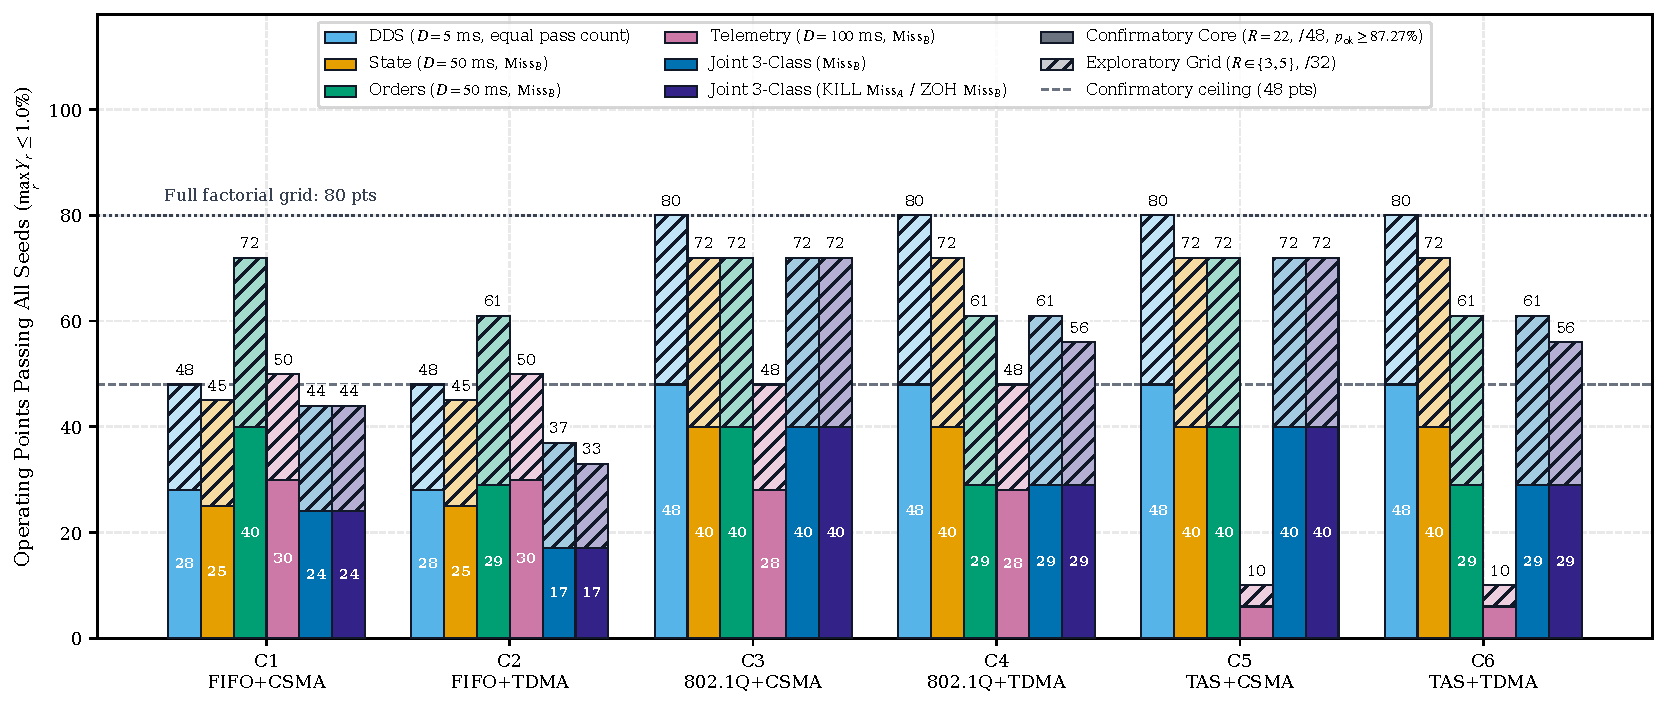
\includegraphics[width=0.95\textwidth]{images/pdf/fig_conformance_bars.pdf}
\caption{Stratified distribution-free operating-envelope counts ($\max_{r \le R} Y_r \le \qty{1.0}{\percent}$ on \texttt{supp-maxR}) stacked into Confirmatory Core ($\Namr \in \{10, 40, 80\}$, $R=22$, solid bottom out of $48$ points, $p_{\mathrm{ok}} \ge \qty{87.27}{\percent}$) and Exploratory Grid ($\Namr \in \{5, 20\}$, $R \in \{3, 5\}$, hatched top out of $32$ points), comparing per-class counts against Joint 3-Class ($\MissB$ and Watchdog KILL-A / ZOH-B).}
\label{fig:conformance_bars}
\end{figure}

\begin{figure}[!tb]
\centering
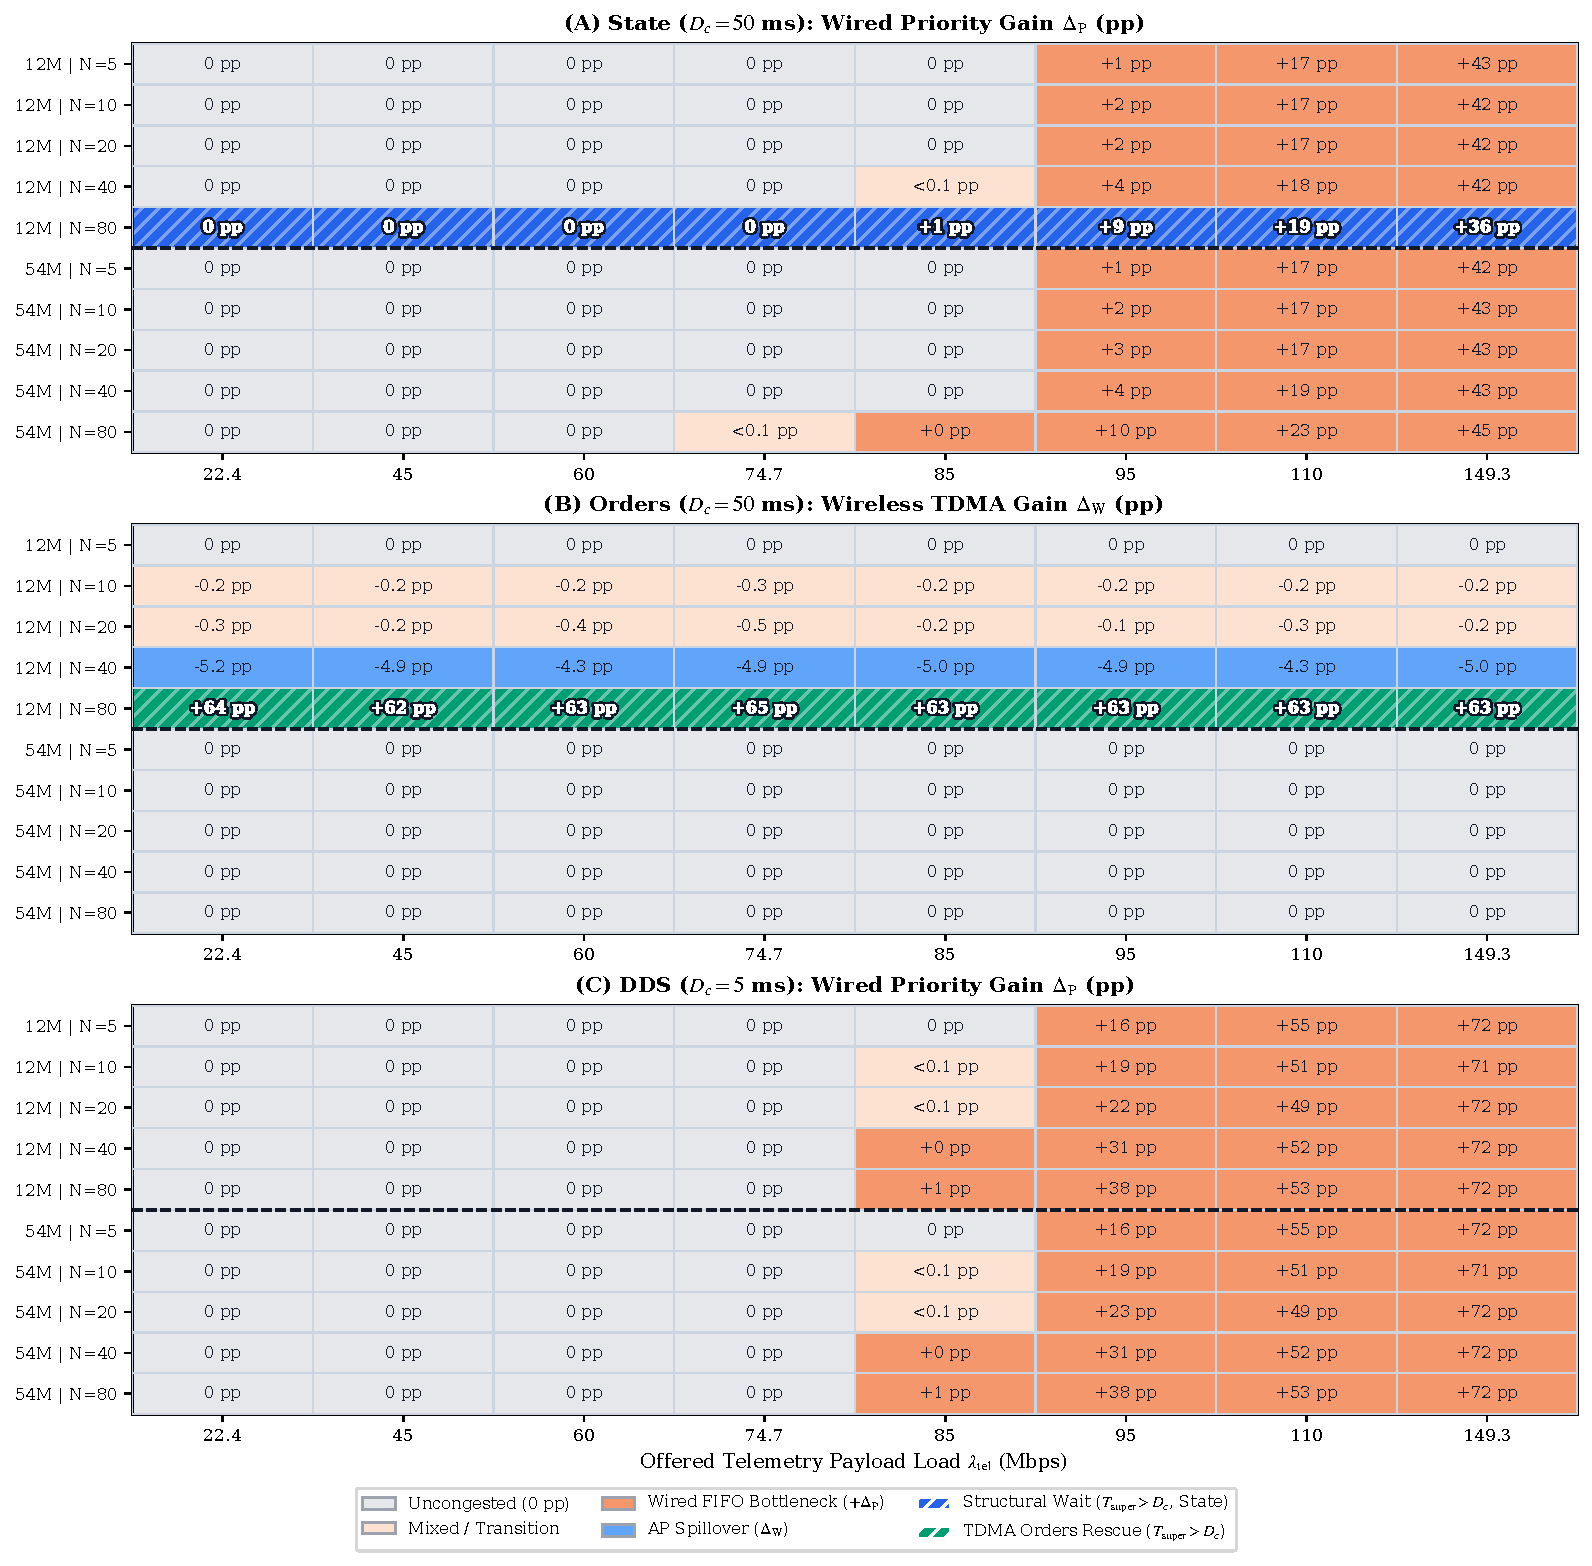
\includegraphics[width=0.82\textwidth]{images/pdf/fig_migration_heatmaps.pdf}
\caption{Full $80$-point bottleneck migration regime map on \texttt{supp-maxR}: (A)~State companion-averaged wired gain ($\GainPbar$ in \si{\pp}, with hatched dual-stress structural barrier at $\Tsuper > D_c$); (B)~Orders TDMA gain ($\GainWpair$ in \si{\pp}, highlighting AP spillover at $\Namr=40,\; \qty{12}{\mbps}$, transition regime at $\Namr=10,\; \qty{12}{\mbps}$, and hatched rescue at $\Namr=80,\; \qty{12}{\mbps}$); (C)~DDS companion-averaged wired gain ($\GainPbar$ in \si{\pp}). Panels plot uniform $\MissB$ contrasts across all $80$ points; Watchdog-enforced $\MissA$ values appear in \Cref{tab:aggregate_performance,tab:selected_points,tab:dual_stress_matrix,tab:conformance_summary}.}
\label{fig:migration_heatmaps}
\end{figure}

\paragraph{Bottleneck Migration Regime Map and Stratified Operating-Envelope Screen.}
\Cref{tab:migration_regimes,tab:conformance_summary} and \Cref{fig:conformance_bars,fig:migration_heatmaps} synthesize the migration map across all $80$ grid points. In \Cref{fig:migration_heatmaps}A, row \texttt{12M | N=80} at $\ltel \in \{95.0, 110.0, 149.3\}\,\text{Mbps}$ displays the co-occurrence of the structural TDMA barrier ($\Tsuper = \qty{90}{\milli\second} > \qty{50}{\milli\second}$) and wired FIFO saturation ($\GainP = \qty{+9}{\pp}$ to \qty{+36}{\pp}), while \Cref{fig:migration_heatmaps}B isolates AP block burst spillover at \texttt{12M | N=40} ($\Tsuper=\qty{42}{\milli\second}$). Replacing legacy packet-level Wilson/Student-$t$ screening with the stratified distribution-free order-statistic screen (\Cref{tab:conformance_summary} and \Cref{fig:conformance_bars}) eliminates branch non-monotonicity and cleanly separates the Confirmatory Core from the Exploratory Grid. On the $48$ Confirmatory points ($\Namr \in \{10, 40, 80\}$, $R=22$, where passing guarantees $p_{\mathrm{ok}} \ge \qty{87.27}{\percent}$), every critical class in Cells~3 and~5 exhibits \emph{zero} Mixed points (All $> \qty{1}{\percent}$ cleanly isolates the $(\Namr=80,\; \qty{12}{\mbps})$ failure rows instead of marking right-skewed CSMA slices unresolved), passing $40/48$ (\qty{83.3}{\percent}: all $24/24$ at \qty{54}{\mbps} plus all $16/16$ at $\Namr \in \{10, 40\},\; \qty{12}{\mbps}$); Cells~4 and~6 pass all $24/24$ Confirmatory points at \qty{54}{\mbps} and $5/24$ at \qty{12}{\mbps} ($29/48 = \qty{60.4}{\percent}$ under both $\MissB$ and Watchdog $\MissA$), with three Mixed Confirmatory TDMA Orders slices at $(\Namr=10,\; \qty{12}{\mbps},\; \ltel \in \{45.0, 74.7, 149.3\}\,\text{Mbps})$ where single-seed tails reach $\MissB \in \qtyrange{1.0004}{1.0454}{\percent}$ and $\MissA \in \qtyrange{1.298}{1.492}{\percent}$ ($1$ to $2$ of $22$ seeds exceeding \qty{1}{\percent} because $K=1$ on $\Tsuper = \qty{10}{\milli\second}$ overflows on any cycle burst of $\ge 2$ orders). Across all $80$ points, Cells~4 and~6 pass $40/40$ (\qty{100}{\percent}) points at \qty{54}{\mbps} under both metrics (noting that Cell~6 State at $\Namr=80,\; \qty{54}{\mbps}$ has max single-packet delay \qty{50.20}{\milli\second}, yielding $\MissB = \qty{0.00}{\percent}$ and $\MissA = \qty{0.0023}{\percent} \ll \qty{1.0}{\percent}$ vs.\ Cell~4 max \qty{48.36}{\milli\second}), and reach $61/80$ (\qty{76.2}{\percent}) under $\MissB$ vs.\ $56/80$ (\qty{70.0}{\percent}) under Watchdog KILL-A / ZOH-B, as five additional Exploratory $(\Namr=20,\; \qty{12}{\mbps})$ TDMA Orders slices ($K=3$ on $\Tsuper = \qty{20}{\milli\second}$, $\Pr[\mathrm{Pois}(2.0) > 3] = \qty{14.3}{\percent}$) show single-seed $\MissA \in \qtyrange{1.05}{1.39}{\percent}$ ($32/32$ Exploratory under $\MissB$ vs.\ $27/32 = \qty{84.4}{\percent}$ under Watchdog KILL-A). Finally, DDS in Cells~3 to~6 passes all $80/80$ points under both metrics, while secondary Joint 4-Class counts (\qtyrange{10.0}{11.2}{\percent} in Cells~5/6) remain dominated by elastic Telemetry above the uniform \qty{44.8}{\mbps} GCL ceiling.

% =============================================================================
\section{Supporting Studies: Wireless Diagnostics, NER Interface, Lookup Accuracy, and Schedule Sensitivity}
\label{sec:supporting}

\subsection{Contention Seed Skewness, Spatial Capture, and Fixed-Phase TAS Gating}
\label{sec:micro_diagnostics}

At $(\Namr=80,\; \qty{12}{\mbps},\; \qty{22.4}{\mbps})$, comparing \Cref{fig:domain_bars}B against \Cref{fig:ecdf_n80}B reveals why the packet-weighted pooled mean State delay in CSMA/CA Cells~1 and~3 (\qty{81.36}{\milli\second}) exceeds TDMA Cell~2 (\qty{45.92}{\milli\second}) even though the median $p_{50}$ in Cells~1 and~3 is only \qty{4.44}{\milli\second} (vs.\ \qty{45.93}{\milli\second} in Cell~2). To prevent optional-stopping distortion from merging post-hoc collapse sampling with the triggering exploratory batch, \Cref{tab:collapse_incidence} reports the pre-extension sample ($r = 0..21$, $n=22$), the unbiased independent confirmation batch ($r = 22..44$, $n=23$), and the descriptive pooled ensemble ($R=45$, \Cref{fig:wireless_diagnostics}A). In Cell~1, the independent confirmation batch records $0/23$ runaway collapses ($\ge \qty{50}{\percent}$, Clopper--Pearson \qty{95}{\percent} CI $[\qty{0.00}{\percent}, \qty{14.82}{\percent}]$) and $3/23$ (\qty{13.04}{\percent}, CI $[\qty{2.78}{\percent}, \qty{33.59}{\percent}]$) intermediate contention stalls (seeds $r=42$ at \qty{12.62}{\percent}, $r=23$ at \qty{27.75}{\percent}, and $r=28$ at \qty{48.39}{\percent}); pooled descriptively across $R=45$, $41/45$ (\qty{91.1}{\percent}) remain below \qty{10}{\percent} (median \qty{2.39}{\percent}) and only triggering seed $r=3$ reaches collapse ($\MissB = \qty{76.13}{\percent}$, $p_{99} = \qty{10683.0}{\milli\second}$ in single-seed ECDF), dominating the \qty{6.03}{\percent} $R=22$ mean. Across all eight loads on the same $22$ \texttt{rng-2} layouts ($176$ runs, \Cref{tab:collapse_incidence}), Cells~3 and~5 both incur $13/176$ (\qty{7.39}{\percent}) runaway collapses (\qtyrange{16.48}{17.61}{\percent} stalls $\ge \qty{10}{\percent}$), confirming that heavy-tailed contention collapse is a structural property of unfavorable AMR layouts rather than a one-seed artifact.

\begin{table}[!tb]
\centering
\scriptsize
\setlength{\tabcolsep}{2.0pt}
\caption{Three-regime seed classification at $(\Namr=80,\; \qty{12}{\mbps},\; \ltel=\qty{22.4}{\mbps})$ for Cell~1 split between pre-extension ($r=0..21$), unbiased independent confirmation ($r=22..44$, exact Clopper--Pearson 95\% CIs), and descriptive pooled ($R=45$), plus empirical Cell~3 and Cell~5 rates across $176$ runs ($8\text{ loads} \times 22$ shared \texttt{rng-2} layouts, reported descriptively without i.i.d.\ binomial CIs).}
\label{tab:collapse_incidence}
\begin{tabular}{@{}l r r r r c@{}}
\toprule
\textbf{Cell / Sample Batch} & \textbf{Threshold $\tau$} & \textbf{Runs $n$} & \textbf{Exceed $k$} & \textbf{Incidence} & \textbf{Clopper--Pearson 95\% CI} \\
\midrule
Cell 1 Pre-extension ($r=0..21$) & $\ge \qty{10.0}{\percent}$ & 22 & 1 & \qty{4.55}{\percent} & $[\qty{0.12}{\percent},\; \qty{22.84}{\percent}]$ \\
 & $\ge \qty{50.0}{\percent}$ & 22 & 1 & \qty{4.55}{\percent} & $[\qty{0.12}{\percent},\; \qty{22.84}{\percent}]$ \\
\midrule
Cell 1 Confirm.\ ($r=22..44$) & $\ge \qty{10.0}{\percent}$ & 23 & 3 & \qty{13.04}{\percent} & $[\qty{2.78}{\percent},\; \qty{33.59}{\percent}]$ \\
 & $\ge \qty{25.0}{\percent}$ & 23 & 2 & \qty{8.70}{\percent} & $[\qty{1.07}{\percent},\; \qty{28.04}{\percent}]$ \\
 & $\ge \qty{50.0}{\percent}$ & 23 & 0 & \qty{0.00}{\percent} & $[\qty{0.00}{\percent},\; \qty{14.82}{\percent}]$ \\
 & $\ge \qty{70.0}{\percent}$ & 23 & 0 & \qty{0.00}{\percent} & $[\qty{0.00}{\percent},\; \qty{14.82}{\percent}]$ \\
\midrule
Cell 1 Pooled ($R=45$) & $\ge 10/25/50/70\%$ & 45 & 4/3/1/1 & 8.9/6.7/2.2/\qty{2.2}{\percent} & (descriptive post-hoc pool) \\
\midrule
Cell 3 (80, 12M, $8\times 22$ runs) & $\ge 10 / 25 / \qty{50}{\percent}$ & 176 & 29 / 23 / 13 & 16.5 / 13.1 / \qty{7.39}{\percent} & (layout-clustered rate) \\
Cell 5 (80, 12M, $8\times 22$ runs) & $\ge 10 / 25 / \qty{50}{\percent}$ & 176 & 31 / 26 / 13 & 17.6 / 14.8 / \qty{7.39}{\percent} & (layout-clustered rate) \\
\bottomrule
\end{tabular}
\end{table}

\begin{figure}[!tb]
\centering
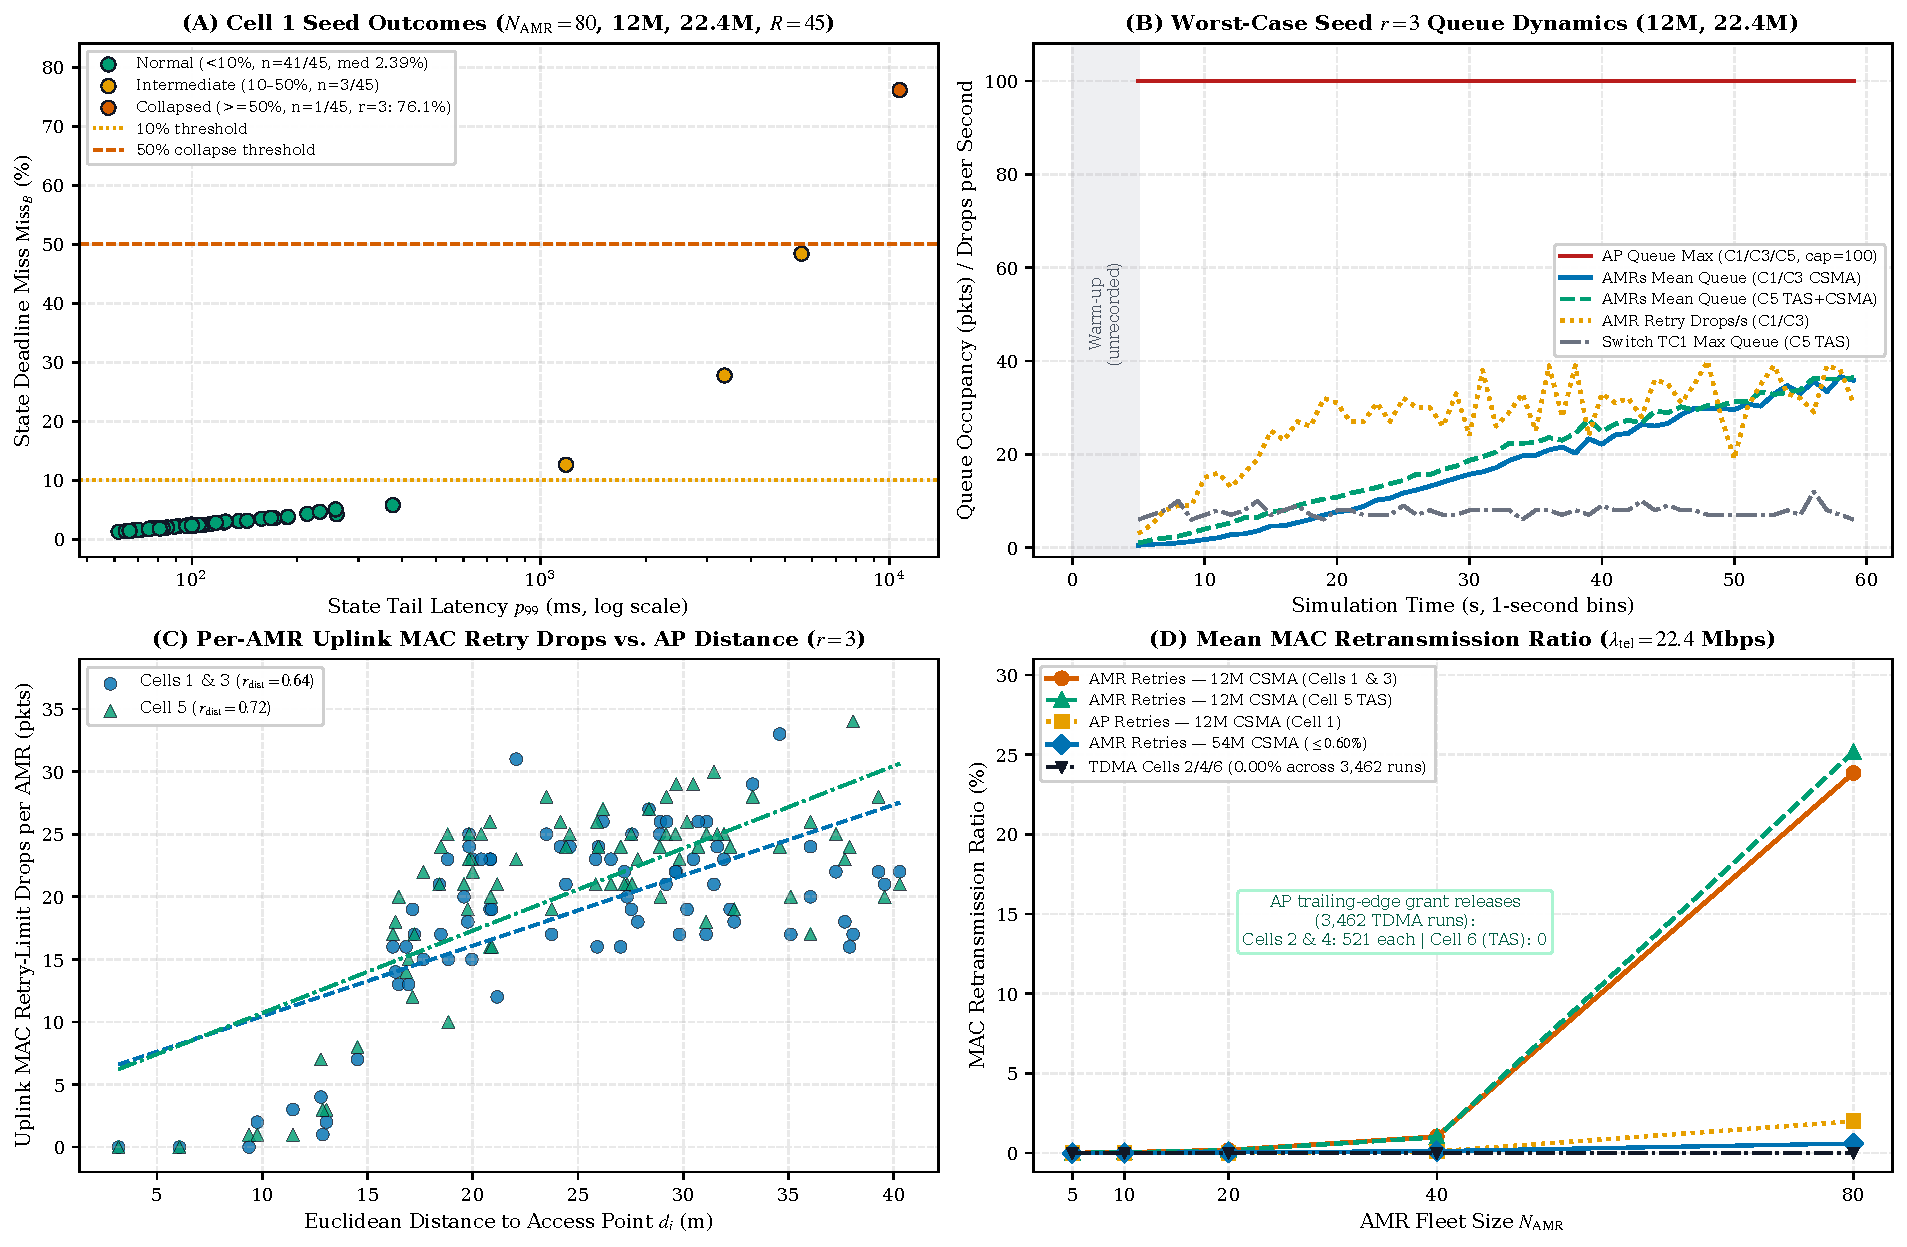
\includegraphics[width=0.95\textwidth]{images/pdf/fig_wireless_diagnostics.pdf}
\caption{Wireless contention and micro-architectural diagnostics: (A)~Cell~1 three-regime seed distribution across $R=45$ seeds at $(\Namr=80,\; \qty{12}{\mbps},\; \qty{22.4}{\mbps})$; (B)~worst-case seed $r=3$ 1-second post-warm-up queue occupancy and retry-drop evolution with $[0, 5]\,\text{s}$ warm-up shaded; (C)~observational correlation $\rdist$ between Euclidean distance to the AP ($d_i$) and per-AMR uplink MAC retry drops on $r=3$; (D)~mean MAC retransmission ratios across fleet sizes ($0$ retries in all \num{3462} TDMA runs) with annotated AP grant-release summary ($521$ vs.\ $0$ under fixed zero-offset phase).}
\label{fig:wireless_diagnostics}
\end{figure}

To inspect the mechanics of this worst-case collapse, we recorded full vector traces on seed $r=3$ across CSMA/CA Cells~1, 3, and~5 (\Cref{fig:wireless_diagnostics}B and C). Because $r=3$ is the sole collapsed seed in the 45-seed ensemble, these diagnostics characterize a worst-case pathology rather than typical behavior. From the first post-warm-up second ($t=\qty{5}{\second}$, already at its 100-packet maximum) through $t=\qty{60}{\second}$, the AP pending queue remains saturated (mean occupancy \qty{99.61}{\pkt} in Cells~1/3, \qty{99.64}{\pkt} in Cell~5), dropping \num{15450} downlink Orders frames in Cells~1/3 (\num{15659} in Cell~5, $0$ retry drops), while uplink AMR queues grow monotonically (post-warm-up mean \qty{17.27}{\pkt} in Cells~1/3, \qty{19.49}{\pkt} in Cell~5), incurring \num{1499} AMR MAC retry drops and \num{218} queue drops in Cells~1/3 (\num{1631} and \num{346} in Cell~5). Across the $80$ AMRs in $r=3$ ($d_i \in [\qty{3.17}{\meter}, \qty{40.29}{\meter}]$), Euclidean distance to the AP correlates strongly with uplink AMR retry drops ($\rdist = +0.644$ in Cells~1/3, $+0.718$ in Cell~5: distant \texttt{amr[77]} at \qty{34.59}{\meter} suffers $33$ retry drops in Cells~1/3 vs.\ $0$ for nearby \texttt{amr[34]} at \qty{3.17}{\meter}) and weakly negatively with delivered Orders ($\rdist = -0.229$ / $-0.154$); under free-space path loss ($\alpha=2.0$), a $>10\times$ distance ratio produces $> \qty{20}{\decibel}$ received-power differential at the AP consistent with SNIR physical capture~\cite{lee2007experimental}, leaving a controlled distance or capture ablation to future work.

Finally, across all \num{3462} Scheduled TDMA runs (\Cref{fig:wireless_diagnostics}D; Cells~2: \num{1154}, 4: \num{1154}, 6: \num{1154}), wireless MAC retransmissions, retry drops, and AMR grant releases are zero. At the AP, unpaced wired switches (Cells~2 and~4) record $521$ trailing-edge DIFS channel-grant releases each when Poisson Orders arrivals fall within \qty{28}{\micro\second} of the merged AP block cutoff, whereas Cell~6 (802.1Qbv TAS) records $0$ across \num{1154} runs (\Cref{fig:wireless_diagnostics}D). Crucially, this $521 \to 0$ reduction is a consequence of our fixed zero-offset GCL-to-TDMA phase relation rather than a phase-invariant property of TAS: under Cell~6, Orders frames finish traversing \texttt{eth[1]} inside $[53.3, 100.0)\,\mu\text{s} \pmod{\qty{1}{\milli\second}}$ (with physical frame completion at \qty{52.32}{\micro\second} prior to the \qty{0.96}{\micro\second} trailing Ethernet IFG), which misses all ten TDMA $28\,\mu\text{s}$ trailing-edge danger windows at \texttt{cyclePhaseOffset = 0} (clearing the nearest cutoffs by just \qty{2.0}{\micro\second} at $\Namr=20,\; \qty{12}{\mbps}$ and \qty{2.3}{\micro\second} at physical arrival---or \qty{3.3}{\micro\second} including IFG---at $\Namr=40,\; \qty{12}{\mbps}$). Shifting either offset modulo \qty{1}{\milli\second} into one of those $28\,\mu\text{s}$ windows would re-introduce AP grant releases.

\subsection{Multi-Rate NER Tick Sensitivity and ZOH Excess Staleness}
\label{sec:ner_multirate}

To evaluate multi-rate digital-twin execution, \Cref{tab:ner_multirate} and \Cref{fig:ner_interface}A and B examine how widening the NER consumption tick $T \in \{10, 50, 500\}\,\text{ms}$ and replacing the class budget $L_c = D_c$ with the tick period $L_c = T$ (variant $B^T$) affect miss rates, Watchdog TTL discards, and ZOH excess tick staleness $\Delta k_{\mathrm{stale},T}$ on delivered State frames.

\begin{table}[!tbp]
\centering
\footnotesize
\setlength{\tabcolsep}{3.0pt}
\caption{Multi-rate NER tick sensitivity ($\MissA$, $\MissB$ at $T \in \{10, 50, 500\}\,\text{ms}$, variant $B^T$ at $L_c=T=\qty{10}{\milli\second}$) and ZOH excess staleness $\Delta k_{\mathrm{stale},10}$ on delivered State packets (packet-weighted per scenario and averaged equally across all $80$ operating points, matching the miss-rate and TTL columns; the $16$-point $\Namr=80$ slice means are $5.06 / 0.56 / 5.04 / 5.93 / 0.47$ ticks for C1 / C2 / C3 / C5 / C4\&C6, with global maxima \num{1613} ticks $=\qty{16.13}{\second}$ and \num{1913} ticks $=\qty{19.13}{\second}$) or continuous Watchdog TTL discard rates ($a > g + D_c$ on delivered frames; unweighted scenario means on $80$-point \texttt{supp-maxR} for State/Orders and \texttt{core-R3}/\texttt{supp-maxR} for DDS). All $T$ columns use the fixed primary $c(\qty{100}{\milli\second}, \qty{10}{\milli\second}) \le \qty{60.0}{\second}$ horizon set $\mathcal{V}$, where $p_{\mathrm{late}}$ bounds miss-rate changes from resolving terminal in-flight packets on $\mathcal{V}$; adopting a shared $c(\qty{100}{\milli\second}, \qty{500}{\milli\second}) \le \qty{60.0}{\second}$ cutoff would also exclude up to \qty{0.89}{\percent} (\qty{0.45}{\percent} mean) of final-half-second arrivals from the denominator.}
\label{tab:ner_multirate}
\begin{tabular}{@{}l l r r r r r l@{}}
\toprule
\textbf{Class} & \textbf{Pool / Cells} & \textbf{$\MissA$} & \multicolumn{3}{c}{\textbf{$\MissB(T)$}} & \textbf{$B^T$} & \textbf{TTL kill (\%) or ZOH $\Delta k_{\mathrm{stale},10}$} \\
\cmidrule(lr){4-6}
 & & \textbf{(\%)} & \textbf{\qty{10}{\milli\second}} & \textbf{\qty{50}{\milli\second}} & \textbf{\qty{500}{\milli\second}} & \textbf{(\%)} & \textbf{(mean / max)} \\
\midrule
DDS & core-R3 C1/C2 & 45.55 & 24.28 & 15.90 & 13.97 & 13.77 & TTL $31.78$ / $90.7$ \\
 & supp-maxR C1/C2 & 35.44 & 18.66 & 11.40 & 9.76 & 9.58 & TTL $25.86$ / $90.6$ \\
 & C3 to C6 & \textbf{0.00} & \textbf{0.00} & \textbf{0.00} & \textbf{0.00} & \textbf{0.00} & TTL $0.00$ \\
\midrule
State & C1 (FIFO+CSMA) & 8.93 & 8.89 & 8.80 & 8.58 & 10.66 & $1.01$ / \num{1613} ticks \\
 & C2 (FIFO+TDMA) & 12.98 & 12.11 & 10.02 & 8.21 & 40.63 & $0.11$ / \textbf{5} ticks \\
 & C3 (802.1Q+CSMA) & 0.98 & 0.95 & 0.86 & 0.64 & 1.98 & $1.01$ / \num{1612} ticks \\
 & C5 (TAS+CSMA) & 1.05 & 1.02 & 0.93 & 0.70 & 2.09 & $1.19$ / \num{1913} ticks \\
 & C4/C6 (TDMA) & 4.57 & 4.02 & 1.88 & \textbf{0.19} & 28.10 & $0.09$ / \textbf{5} ticks \\
\midrule
Orders & C1/C3/C5 (CSMA) & 9.54 & 9.50 & 9.34 & 4.70 & 9.79 & TTL $7.94$ / $84.7$ \\
 & C2/C4/C6 (TDMA) & 4.74 & 3.73 & 1.50 & \textbf{0.16} & 27.22 & TTL $4.74$ / $40.0$ \\
\bottomrule
\end{tabular}
\end{table}

\begin{figure}[!tbp]
\centering
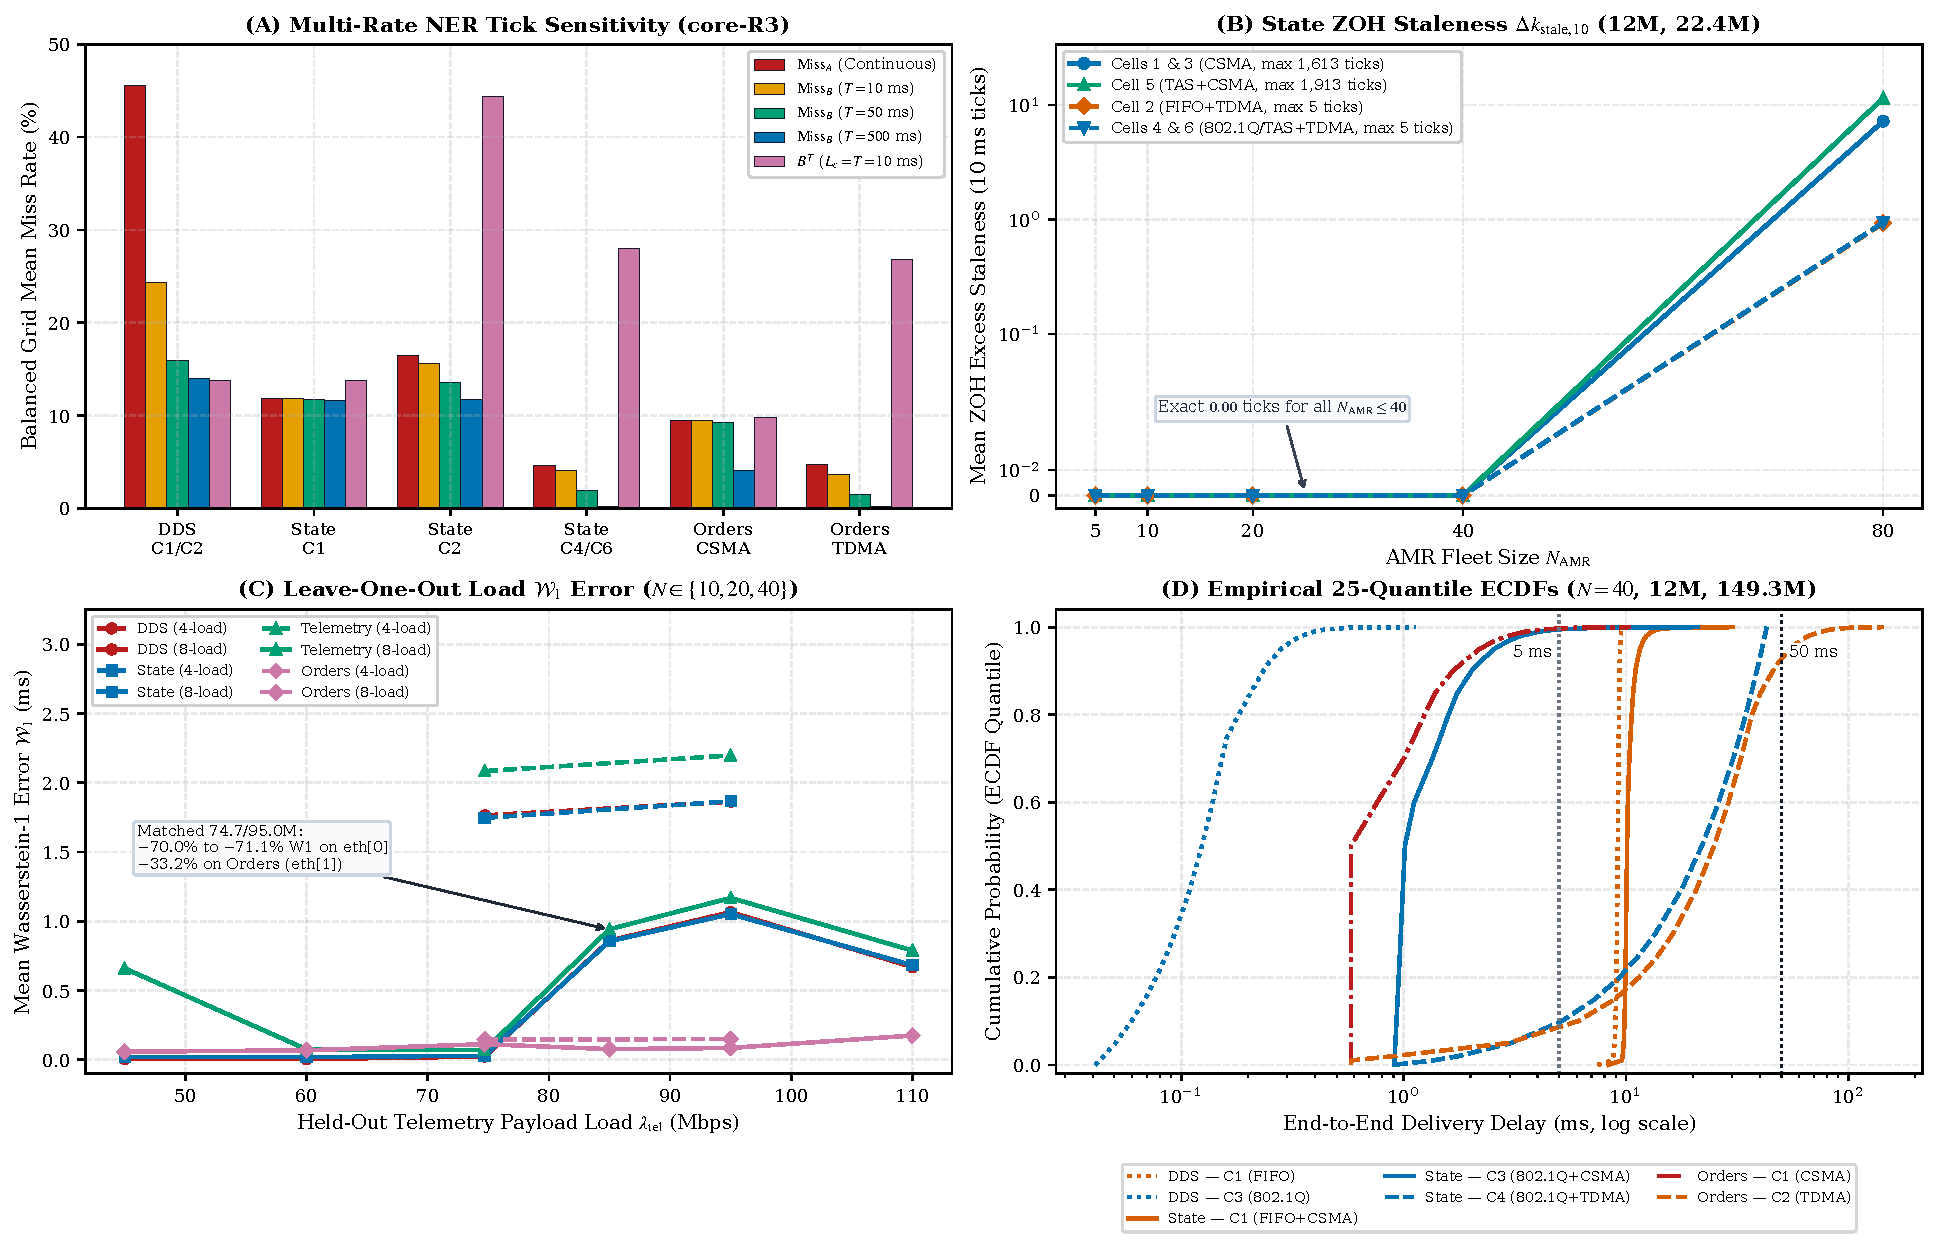
\includegraphics[width=0.95\textwidth]{images/pdf/fig_ner_interface.pdf}
\caption{Digital Twin NER interface and Leave-One-Out PCHIP lookup validation: (A)~multi-rate tick sensitivity on \texttt{core-R3}; (B)~delivered State ZOH excess staleness $\Delta k_{\mathrm{stale},10}$ across $\Namr$ at $(\qty{12}{\mbps},\; \qty{22.4}{\mbps})$, with legend peaks reporting global \texttt{supp-maxR} maxima across all $80$ points; (C)~Leave-One-Out load-axis $\Wone$ MAE comparing the 4-load \texttt{core-R3} and 8-load \texttt{knee-R3} grids across matched $(\Namr \in \{10, 20, 40\})$; (D)~empirical 25-quantile ECDFs from \texttt{supp-maxR} at $(\Namr=40,\; \qty{12}{\mbps},\; \qty{149.3}{\mbps},\; R=22)$ showing Cell~4 State bounded below \qty{43.0}{\milli\second} ($\Tsuper=\qty{42}{\milli\second}$) while Cell~2 Orders cross \qty{50}{\milli\second} ($p_{99}=\qty{75.6}{\milli\second}$) due to 10-slot spillover.}
\label{fig:ner_interface}
\end{figure}

Because KILL classes (DDS and Orders) are discarded continuously by Watchdog TTL whenever $a > g + D_c$, \Cref{tab:ner_multirate} contrasts continuous Watchdog unavailability ($\MissA$) against pure tick-grid arrival timeliness ($\MissB$ without an intervening continuous watchdog): for DDS under wired FIFO (Cells~1/2), evaluating $\MissB$ on the $T = \qty{10}{\milli\second}$ tick grid lowers the miss count by \qty{21.27}{\pp} relative to $\MissA$ in \texttt{core-R3} ($\MissA = \qty{45.55}{\percent}$ vs.\ $\MissB = \qty{24.28}{\percent}$) solely because the \qty{9.41}{\milli\second} FIFO drain ceiling falls within $[D_c, D_c + T) = [\qty{5}{\milli\second}, \qty{15}{\milli\second})$, whereas an active continuous Watchdog TTL still discards \qty{31.78}{\percent} (\texttt{supp-maxR}: \qty{25.86}{\percent}) of valid generated DDS frames prior to tick consumption (leaving \qty{13.77}{\percent} / \qty{9.58}{\percent} physically dropped). Similarly, TDMA Orders exhibits Watchdog $\MissA = \qty{4.74}{\percent}$ vs.\ counterfactual tick-grid $\MissB(\qty{10}{\milli\second}) = \qty{3.73}{\percent}$, with all \qty{4.74}{\percent} late frames discarded by the Watchdog TTL. Conversely, evaluating variant $B^T$ ($L_c = T = \qty{10}{\milli\second}$) tightens the budget of State and Orders from \qty{50}{\milli\second} to \qty{10}{\milli\second}, elevating TDMA State misses to \qty{28.10}{\percent} across \texttt{supp-maxR} (Cells~4/6) because $\Tsuper \in \{20, 42, 48, 90\}\,\text{ms}$ exceeds \qty{10}{\milli\second} at every configuration with $\Namr \ge 20$ at \qty{12}{\mbps} PHY or $\Namr \ge 40$ at \qty{54}{\mbps} PHY.

On delivered State frames, Scheduled TDMA (Cells~2, 4, and~6) limits worst-case observed ZOH excess staleness across all $80$ operating points (\num{6924} paired runs) to $\Delta k_{\max} = \qty{5}{\tick}$ at $T=\qty{10}{\milli\second}$ (\qty{50}{\milli\second} excess age; $\Delta k_{\max} = 1\text{ tick}$ at $T \in \{50, 500\}\,\text{ms}$), whereas CSMA/CA freezes delivered State for up to $\num{1494} / 299 / \qty{30}{\tick}$ ($\approx \qty{14.94}{\second}$) in Cells~1/3 and $\num{1913} / 382 / \qty{38}{\tick}$ ($\approx \qty{19.13}{\second}$) in Cell~5 at $(\Namr=80,\; \qty{12}{\mbps},\; \qty{22.4}{\mbps})$, and up to $\num{1613} / 323 / \qty{33}{\tick}$ (Cell~1) and $\num{1612} / 323 / \qty{33}{\tick}$ (Cell~3) at $\ltel = \qty{149.3}{\mbps}$ (\Cref{fig:ner_interface}B). Note that $\Delta k_{\mathrm{stale}}$ excludes undelivered frames; in Cell~2 under dual stress, \qty{42.2}{\percent} wired switch drops induce additional consecutive-update staleness gaps not reflected in delivered-packet $\Delta k_{\mathrm{stale}}$.

\subsection{Leave-One-Out Wasserstein PCHIP Lookup Accuracy}
\label{sec:pchip_accuracy}

To replay empirical network delays inside a fast digital twin without re-simulating every packet, the lookup module treats each simulated operating point as a conditional delivery-delay ECDF stored via 25 quantile knots $F^{-1}(q)$ plus physical drop probability $\ploss$. For an intermediate query $(\Namr, \ltel)$, 2D quantile-space PCHIP fits shape-preserving Fritsch--Butland monotone piecewise cubic Hermite splines~\cite{fritsch1984pchip} through each quantile level (clamping post-saturation queries to nearest neighbor without extrapolation), followed by an explicit cumulative-maximum non-crossing guard across the 25 quantile levels and non-negativity clipping ($\ge 0$). Discrepancy between a predicted quantile function $F_{\mathrm{pred}}^{-1}$ and held-out empirical ECDF $F_{\mathrm{emp}}^{-1}$ is measured by the 1D Wasserstein distance $\Wone(F_{\mathrm{pred}}, F_{\mathrm{emp}}) = \int_0^1 |F_{\mathrm{pred}}^{-1}(q) - F_{\mathrm{emp}}^{-1}(q)|\,dq$ (\si{\milli\second})~\cite{panaretos2019wasserstein}, alongside absolute errors in $\MissB(D_c)$, $\ploss$, $p_{50}$, and $p_{99}$. \Cref{tab:pchip_loo,tab:pchip_axes} report Leave-One-Out (LOO) cross-validation errors across both grid axes.

\begin{table}[!tb]
\centering
\footnotesize
\setlength{\tabcolsep}{2.2pt}
\caption{Matched load-axis comparison of 4-load (\texttt{core-R3}) versus 8-load (\texttt{knee-R3}) LOO PCHIP lookup interpolation ($\Namr \in \{10,20,40\}$, held-out $\ltel \in \{74.7, 95.0\}\,\text{Mbps}$, $n=72$ series per class, reporting MAE across held-out series).}
\label{tab:pchip_loo}
\begin{tabular}{@{}l l r r r r r r@{}}
\toprule
\textbf{Class ($D_c$)} & \textbf{Path / Trunk} & \multicolumn{2}{c}{\textbf{Mean $\Wone$ (ms)}} & \multicolumn{2}{c}{\textbf{Mean $|e(p_{99})|$ (ms)}} & \multicolumn{2}{c}{\textbf{MAE $|e(\MissB)|$ (pp)}} \\
\cmidrule(lr){3-4} \cmidrule(lr){5-6} \cmidrule(lr){7-8}
 & & \textbf{4-Load} & \textbf{8-Load ($\Delta\%$)} & \textbf{4-Load} & \textbf{8-Load} & \textbf{4-Load} & \textbf{8-Load} \\
\midrule
DDS (\qty{5}{\milli\second}) & \texttt{eth[0]} (shared) & 1.815 & \textbf{0.545 ($-$70.0\%)} & 2.251 & 0.560 & 5.56 & \textbf{3.11} \\
State (\qty{50}{\milli\second}) & \texttt{eth[0]} + Wlan & 1.807 & \textbf{0.541 ($-$70.1\%)} & 2.290 & 0.640 & 0.47 & \textbf{0.30} \\
Telemetry (\qty{100}{\milli\second}) & \texttt{eth[0]} (shared) & 2.141 & \textbf{0.619 ($-$71.1\%)} & 2.530 & 0.619 & 5.10 & \textbf{2.52} \\
Orders (\qty{50}{\milli\second}) & \texttt{eth[1]} (dedic.) & 0.148 & \textbf{0.099 ($-$33.2\%)} & 0.935 & 0.771 & 0.13 & \textbf{0.09} \\
\bottomrule
\end{tabular}
\end{table}

\begin{table}[!tb]
\centering
\scriptsize
\setlength{\tabcolsep}{3.0pt}
\caption{Full LOO cross-validation of the 1D Wasserstein PCHIP lookup along the fleet axis (leave-one-fleet-size-out) and load axis (leave-one-load-out), reported as mean absolute errors across all $n$ held-out series ($|e(\MissB)|, |e(\ploss)|$ in \si{\pp}; $|e(p_{50})|, |e(p_{99})|, \Wone$ in \si{\milli\second}).}
\label{tab:pchip_axes}
\begin{tabular}{@{}l l r r r r r r@{}}
\toprule
\textbf{Class} & \textbf{LOO Axis \& Pool ($n$)} & \textbf{$|e(\ploss)|$} & \textbf{$|e(\MissB)|$} & \textbf{$|e(p_{50})|$} & \textbf{$|e(p_{99})|$} & \textbf{Mean $\Wone$} & \textbf{Med.\ $\Wone$} \\
 & & \textbf{(pp)} & \textbf{(pp)} & \textbf{(ms)} & \textbf{(ms)} & \textbf{(ms)} & \textbf{(ms)} \\
\midrule
DDS & Fleet (core-R3, 144) & 0.03 & 0.15 & 0.007 & 0.003 & 0.009 & 0.001 \\
 & Load (core-R3, 120) & 0.76 & 5.90 & 1.974 & 2.218 & 1.821 & 0.007 \\
 & Load (knee-R3, 216) & 1.15 & \textbf{2.55} & 0.466 & 0.310 & \textbf{0.438} & 0.002 \\
\addlinespace[2pt]
State & Fleet (core-R3, 144) & 0.03 & 0.11 & 0.123 & 3.914 & 0.301 & 0.103 \\
 & Load (core-R3, 120) & 0.65 & 1.13 & 1.933 & 55.384 & 4.032 & 0.028 \\
 & Load (knee-R3, 216) & 0.97 & \textbf{0.97} & 0.454 & 0.393 & \textbf{0.443} & 0.019 \\
\addlinespace[2pt]
Orders & Fleet (core-R3, 144) & 0.10 & 0.62 & 2.800 & 8.321 & 3.031 & 0.176 \\
 & Load (core-R3, 120) & 0.41 & 0.18 & 0.429 & 20.844 & 1.961 & 0.024 \\
 & Load (knee-R3, 216) & 0.00 & \textbf{0.08} & 0.045 & 0.747 & \textbf{0.096} & 0.014 \\
\addlinespace[2pt]
Telemetry & Fleet (core-R3, 144) & 0.01 & 0.01 & 0.008 & 0.006 & 0.010 & 0.002 \\
 & Load (core-R3, 120) & 5.44 & 5.44 & 2.365 & 2.477 & 2.158 & 0.855 \\
 & Load (knee-R3, 216) & 4.66 & \textbf{4.66} & 0.651 & 0.357 & \textbf{0.617} & 0.071 \\
\bottomrule
\end{tabular}
\end{table}

On the strictly matched interior subset ($\Namr \in \{10, 20, 40\}$ at held-out loads $\ltel \in \{74.7, 95.0\}\,\text{Mbps}$, $n=72$ series per class, \Cref{tab:pchip_loo}), refining the telemetry axis from 4 loads to 8 loads reduces mean $\Wone$ by \qtyrange{70.0}{71.1}{\percent} across all three \texttt{eth[0]}-contended classes (DDS: $\qty{1.815}{\milli\second} \to \qty{0.545}{\milli\second}$; State: $\qty{1.807}{\milli\second} \to \qty{0.541}{\milli\second}$; Telemetry: $\qty{2.141}{\milli\second} \to \qty{0.619}{\milli\second}$) and cuts matched DDS MAE $|e(\MissB)|$ from \qty{5.56}{\pp} to \qty{3.11}{\pp} (Telemetry: \qty{5.10}{\pp} $\to$ \qty{2.52}{\pp}). Meanwhile, \Cref{fig:ner_interface}D plots the empirical 25-quantile ECDFs stored by the lookup tables at $(\Namr=40,\; \qty{12}{\mbps},\; \qty{149.3}{\mbps})$, contrasting Cell~1's \qty{9.1}{\milli\second} FIFO queue wall for State/DDS against Cell~4's TDMA State envelope ($\Tsuper=\qty{42}{\milli\second}$, observed max \qty{43.0}{\milli\second}) and Cell~2's spilled TDMA Orders tail crossing \qty{50}{\milli\second} ($p_{99} = \qty{75.6}{\milli\second}$, \Cref{sec:analytical_wireless}). Across all six interior loads of \texttt{knee-R3} ($n=216$, \Cref{tab:pchip_axes}), 8-load interpolation achieves global MAEs of \qty{2.55}{\pp} for DDS (down from \qty{5.90}{\pp} on \texttt{core-R3}), \qty{0.97}{\pp} for State (cutting $|e(p_{99})|$ from \qty{55.38}{\milli\second} to \qty{0.39}{\milli\second}), \qty{0.08}{\pp} for Orders, and \qty{4.66}{\pp} for Telemetry. Because errors concentrate at saturation transitions rather than flat pre-knee loads (\Cref{fig:ner_interface}C: DDS MAE is \qty{0.00}{\pp} across \qtyrange{45.0}{74.7}{\mbps}), local knee errors substantially exceed these global means: on \texttt{knee-R3}, DDS $|e(\MissB)|$ reaches \qty{6.22}{\pp} mean (\qty{25.06}{\pp} max) at \qty{95.0}{\mbps} and \qty{8.72}{\pp} mean (\qty{31.58}{\pp} max) at \qty{110.0}{\mbps}; State reaches \qty{4.95}{\pp} mean (\qty{15.41}{\pp} max) at \qty{110.0}{\mbps}; and Telemetry reaches \qty{7.54}{\pp} mean (\qty{22.68}{\pp} max) at the \qty{45.0}{\mbps} TAS knee and \qty{8.14}{\pp} mean (\qty{13.20}{\pp} max) at \qty{110.0}{\mbps}.

\subsection{Schedule Sensitivity and Co-Design Validation Pilots}
\label{sec:codesign_pilot}

To verify directly in OMNeT++ that the TDMA penalties identified in \Cref{sec:analytical_wireless} arise from finite-$K$ provisioning and trailing AP-block placement rather than inherent limits of scheduled wireless access, we executed an isolated 6-run Cell~4 co-design pilot (\qty{12}{\mbps} PHY, $\ltel = \qty{22.4}{\mbps}$, $R=3$ matched seeds $r \in \{0,1,2\}$; strict five-outcome integer conservation passed, zero wireless retries, \Cref{tab:codesign_pilot}). At $\Namr=40$, expanding the AP block from $K=10$ to $K=12$ within the existing \qty{2.40}{\milli\second} idle cushion preserves $\Tsuper = \qty{42}{\milli\second}$ (\qty{1.28}{\milli\second} slack remaining), cuts downlink Orders $\MissB(\qty{50}{\milli\second})$ from \qty{5.52}{\percent} (matched $R=3$; \qty{5.05}{\percent} in $R=22$ \texttt{supp-maxR}) to \qty{0.18}{\percent} and Watchdog $\MissA$ from \qty{7.99}{\percent} (\texttt{supp-maxR}: \qty{7.27}{\percent}) to \qty{0.41}{\percent} (matching the $M/D^{12}/1$ prediction), and pulls Orders $p_{99}$ from \qty{78.17}{\milli\second} down to \qty{45.07}{\milli\second} ($< D_c$) with \qty{0.00}{\percent} State misses. At $\Namr=80$, replacing the trailing $K=39$ AP block with two symmetric $21$-slot AP sub-blocks spaced \qty{46.00}{\milli\second} apart (\texttt{amr[0..39]} + \qty{11.76}{\milli\second} AP window~1 in $[0, 45.76)\,\text{ms}$, followed by \texttt{amr[40..79]} + \qty{11.76}{\milli\second} AP window~2 in $[46.00, 91.76)\,\text{ms}$; $\Tsuper = \qty{92}{\milli\second}$) eliminates the \qty{15.2}{\pp} block-start wait barrier and multi-cycle overflow, slashing Orders $\MissB(\qty{50}{\milli\second})$ from \qty{31.36}{\percent} to \qty{0.86}{\percent} ($p_{50} = \qty{21.29}{\milli\second}$, $p_{99} = \qty{54.02}{\milli\second}$, $\ploss = \qty{0.00}{\percent}$), while continuous Watchdog $\MissA$ drops from \qty{38.64}{\percent} (\texttt{supp-maxR}: \qty{39.18}{\percent}) to \qty{1.72}{\percent} because \qty{46}{\milli\second} inter-block spacing plus 21-slot serial service slightly exceeds \qty{50}{\milli\second} under peak Poisson bursts. Extending $\Tsuper$ from \qty{90}{\milli\second} to \qty{92}{\milli\second} transparently exposes the uplink single-channel trade-off: State $\MissB(\qty{50}{\milli\second})$ shifts by \qty{+1.66}{\pp} (\qty{39.84}{\percent} $\to$ \qty{41.50}{\percent}, $p_{99} = \qty{92.08}{\milli\second}$, while holding \qty{0.00}{\percent} at $D=\qty{100}{\milli\second}$ and zero physical drops), confirming that joint downlink and uplink compliance below \qty{50}{\milli\second} at $\Namr=80,\; \qty{12}{\mbps}$ requires dual-channel separation or multi-user uplink grants alongside sub-blocked AP transmissions.

\begin{table}[!tbp]
\centering
\scriptsize
\setlength{\tabcolsep}{2.0pt}
\caption{Isolated Cell~4 (802.1Q + TDMA) co-design pilot at $(\qty{12}{\mbps}\text{ PHY},\; \ltel=\qty{22.4}{\mbps},\; R=3\text{ matched seeds})$ versus baseline Cell~4 ($R=3$ matched and \texttt{supp-maxR} reference at $R=22$). Orders rows list $\MissB$ with Watchdog-enforced $\MissA$ in parentheses. All pilot runs recorded zero wireless MAC retries ($\ploss = \qty{0.00}{\percent}$, zero conservation error, and $4$ / $9$ trailing AP grant releases across $3$ runs at $\Namr=40$ / $80$).}
\label{tab:codesign_pilot}
\begin{tabular}{@{}l l r r r r r@{}}
\toprule
\textbf{Pilot Setup} & \textbf{Class} & \textbf{Base $R{=}3$} & \textbf{Base $p_{99}$} & \textbf{Pilot} & \textbf{Quantiles} & \textbf{Supp ($R{=}22$)} \\
\textbf{($\Namr$, AP, $\Tsuper$)} & & \textbf{$\MissB$ ($\MissA$, \%)} & \textbf{(ms)} & \textbf{$\MissB$ ($\MissA$, \%)} & \textbf{$p_{50}/p_{95}/p_{99}$ (ms)} & \textbf{$\MissB$ ($\MissA$, \%)} \\
\midrule
$N{=}40,\; K{=}12$ (\qty{42}{\milli\second}) & Orders & 5.52 (7.99) & 78.17 & \textbf{0.18} (0.41) & 19.05 / 36.01 / \textbf{45.07} & 5.05 (7.27) \\
 & State & 0.00 & 42.48 & \textbf{0.00} & 21.92 / 40.84 / 42.48 & 0.00 \\
\midrule
$N{=}80,\; 2{\times}21$ (\qty{92}{\milli\second}) & Orders & 31.36 (38.64) & 101.24 & \textbf{0.86} (1.72) & 21.29 / 42.31 / \textbf{54.02} & 31.89 (39.18) \\
 & State & 39.84 & 90.00 & 41.50 & 47.15 / 88.36 / 92.08 & 39.90 \\
\bottomrule
\end{tabular}
\end{table}

To test empirically the port-specific switch gating analysis in \Cref{sec:analytical_wired} without altering \texttt{eth[1]} downlink determinism, we executed an isolated 12-run Cell~6 port-rebalancing pilot ($\Namr=40$, \qty{54}{\mbps} PHY, $\ltel \in \{45.0, 60.0, 74.7, 85.0\}\,\text{Mbps}$, $R=3$ matched seeds $r \in \{0,1,2\}$; \qty{10}{\milli\second} \texttt{gateState} vector check, strict five-outcome integer conservation across all \num{4549531} valid pilot packets, bit-identical \texttt{n\_generated\_valid} across all 48 load$\times$class$\times$seed series, and zero wireless retries or AP grant releases, \Cref{tab:gcl_pilot}). Closing the unused TC3 gate on \texttt{eth[0]} while tightening TC2 (DDS) to $[\qty{0}{\micro\second}, \qty{100}{\micro\second})$ and TC1 (State) to $[\qty{100}{\micro\second}, \qty{280}{\micro\second})$ expands TC0 (Telemetry) to \qty{720}{\micro\second} (\qty{67.20}{\mbps} cap) while leaving \texttt{eth[1]} unchanged. Across all four offered loads, all three critical classes preserve \qty{0.00}{\percent} physical drops and \qty{0.00}{\percent} $\MissA$ / $\MissB$ misses (DDS $p_{99} \le \qty{0.99}{\milli\second} \ll \qty{5}{\milli\second}$, Orders $p_{99} = \qtyrange{18.06}{18.10}{\milli\second}$ bit-identical to uniform Cell~6, State $p_{99} \le \qty{20.54}{\milli\second}$). For Telemetry, uniform Cell~6 drops \qty{2.65}{\percent} at \qty{45.0}{\mbps} and \qty{25.24}{\percent} at \qty{60.0}{\mbps} ($R=3$; \qty{2.72}{\percent} and \qty{25.31}{\percent} at $R=22$), whereas rebalanced Cell~6 eliminates \qty{45.0}{\mbps} drops completely (\qty{0.00}{\percent}, $p_{99} = \qty{1.31}{\milli\second}$) and lowers \qty{60.0}{\mbps} misses to \qty{0.13}{\percent} (from finite 20-packet TC0 burst drops at $\rho_{\mathrm{TC0}}=\qty{89.2}{\percent}$). Above the \qty{67.20}{\mbps} gate ceiling, however, non-work-conserving throttling resumes immediately in direct agreement with fluid theory: Telemetry losses reach \qty{10.15}{\percent} at \qty{74.7}{\mbps} (fluid bound \qty{10.04}{\percent}) and \qty{21.00}{\percent} at \qty{85.0}{\mbps} (fluid bound \qty{20.94}{\percent}), compared against \qty{0.006}{\percent} and \qty{0.46}{\percent} under work-conserving IEEE~802.1Q strict priority (Cell~4).

\begin{table}[!tbp]
\centering
\scriptsize
\setlength{\tabcolsep}{1.8pt}
\caption{Isolated 12-run Cell~6 port-specific \texttt{eth[0]} GCL rebalancing pilot ($\Namr=40$, \qty{54}{\mbps} PHY, $R=3$ matched seeds $r \in \{0,1,2\}$; TC3 closed, TC2 \qty{100}{\micro\second}, TC1 \qty{180}{\micro\second}, TC0 \qty{720}{\micro\second} = \qty{67.20}{\mbps} cap; \texttt{eth[1]} unchanged), comparing Telemetry (\qty{100}{\milli\second}) outcomes against uniform Cell~6 TAS and work-conserving Cell~4 802.1Q ($R=3$ matched and \texttt{supp-maxR} $R=22$). Critical classes (DDS, Orders, State) maintain \qty{0.00}{\percent} physical loss and \qty{0.00}{\percent} $\MissA$ / $\MissB$ across all four loads (max $p_{99}$: \qty{0.99}{\milli\second} DDS, \qty{18.10}{\milli\second} Orders, \qty{20.54}{\milli\second} State), with zero wireless retries and bit-identical offered loads.}
\label{tab:gcl_pilot}
\begin{tabular}{@{}r r r r r r r r@{}}
\toprule
\textbf{Offered} & \multicolumn{2}{c}{\textbf{Uniform C6 (500\,$\mu$s)}} & \multicolumn{3}{c}{\textbf{Rebalanced C6 (720\,$\mu$s TC0)}} & \multicolumn{2}{c}{\textbf{802.1Q C4 (Work-Cons.)}} \\
\cmidrule(lr){2-3} \cmidrule(lr){4-6} \cmidrule(lr){7-8}
\textbf{$\ltel$} & \textbf{$R{=}3$ ($R{=}22$)} & \textbf{Base $p_{99}$} & \textbf{Pilot $\MissB/\ploss$} & \textbf{Fluid LB} & \textbf{$p_{50}/p_{95}/p_{99}$} & \textbf{$R{=}3$ ($R{=}22$)} & \textbf{Base $p_{99}$} \\
\textbf{(Mbps)} & \textbf{$\MissB$ (\%)} & \textbf{(ms)} & \textbf{(\%)} & \textbf{(\%)} & \textbf{(ms)} & \textbf{$\MissB$ (\%)} & \textbf{(ms)} \\
\midrule
45.0 & 2.65 (2.72) & 5.19 & \textbf{0.00} & 0.00 & 0.46 / 0.97 / 1.31 & \textbf{0.00} (0.00) & 0.66 \\
60.0 & 25.24 (25.31) & 5.30 & \textbf{0.13} & 0.00 & 0.79 / 2.36 / 3.11 & \textbf{0.00} (0.00) & 0.94 \\
74.7 & 40.01 (40.01) & 5.33 & 10.15 & 10.04 & 3.02 / 3.60 / 3.75 & \textbf{0.006} (0.007) & 1.70 \\
85.0 & 47.33 (47.32) & 5.35 & 21.00 & 20.94 & 3.31 / 3.70 / 3.80 & \textbf{0.46} (0.45) & 2.61 \\
\bottomrule
\end{tabular}
\end{table}

To resolve the buffer-versus-scheduling confound identified on \texttt{eth[0]} in \Cref{sec:rq1} (80-packet shared FIFO buffer vs.\ 20-packet per-class 802.1Q TC0 queue), we executed an isolated 9-run Cell~3 buffer-parity control ablation setting TC0 \texttt{packetCapacity = 80} at $(\Namr=40,\; \qty{54}{\mbps}\text{ PHY},\; \ltel \in \{85.0, 95.0, 149.3\}\,\text{Mbps},\; R=3\text{ matched seeds } r \in \{0,1,2\})$, verified by a \qty{10}{\milli\second} NED parameter check, zero integer conservation discrepancy across \num{5334439} valid pilot packets, and bit-identical offered packet counts across all $36$ load$\times$class$\times$seed series (\Cref{tab:bufparity_pilot}). Expanding TC0 from 20 packets to 80 packets produces three distinct physical regimes: at near-saturation \qty{85.0}{\mbps}, enlarged TC0 absorbs Poisson burst fluctuations completely, lowering Telemetry loss from \qty{0.47}{\percent} (\qty{0.45}{\percent} at $R=22$) to \qty{0.00}{\percent} ($0$ drops across \num{1250753} packets, matching FIFO's \qty{0.00}{\percent} while $p_{99}$ scales from \qty{2.61}{\milli\second} to \qty{4.60}{\milli\second}); at just-saturated \qty{95.0}{\mbps}, enlarging TC0 eliminates \qty{82.9}{\percent} of the excess drop gap over FIFO (\qty{4.85}{\percent} $\to$ \qty{3.96}{\percent} vs.\ \qty{3.77}{\percent} FIFO, leaving only \qty{+0.18}{\pp} from strict priority shielding critical traffic); and under deep saturation at \qty{149.3}{\mbps}, buffer size becomes irrelevant once the backlog pins the queue full, leaving Telemetry loss bit-identical at \qty{38.93}{\percent} (while $p_{99}$ increases $3.5\times$ from \qty{3.01}{\milli\second} to \qty{10.52}{\milli\second} to drain the $4\times$ deeper TC0 queue) and confirming that the \qty{+1.22}{\pp} differential over FIFO (\qty{37.71}{\percent}) arises strictly from priority preemption holding DDS ($p_{99} \le \qty{0.40}{\milli\second}$), State ($p_{99} \le \qty{0.85}{\milli\second}$), and Orders at \qty{0.00}{\percent} loss.

\begin{table}[!tbp]
\centering
\scriptsize
\setlength{\tabcolsep}{1.8pt}
\caption{Isolated 9-run Cell~3 (IEEE~802.1Q) buffer-parity control ablation ($\Namr=40$, \qty{54}{\mbps} PHY, $R=3$ matched seeds $r \in \{0,1,2\}$; TC0 enlarged to 80 packets matching FIFO total capacity), comparing Telemetry (\qty{100}{\milli\second}) outcomes against 80-packet Cell~1 FIFO and baseline 20-packet TC0 Cell~3 ($R=3$ matched and \texttt{supp-maxR} $R=22$). Critical classes (DDS, Orders, State) maintain \qty{0.00}{\percent} loss and misses across all three loads (max critical $p_{99}$: \qty{0.40}{\milli\second} DDS, \qty{0.67}{\milli\second} Orders, \qty{0.85}{\milli\second} State), with bit-identical offered loads.}
\label{tab:bufparity_pilot}
\begin{tabular}{@{}r r r r r r r r@{}}
\toprule
\textbf{Offered} & \textbf{C1 FIFO (80p)} & \multicolumn{2}{c}{\textbf{Base C3 (20p TC0)}} & \multicolumn{4}{c}{\textbf{Control C3 (80p TC0 Buffer-Parity)}} \\
\cmidrule(lr){3-4} \cmidrule(lr){5-8}
\textbf{$\ltel$} & \textbf{$R{=}3$ ($R{=}22$)} & \textbf{$R{=}3$ ($R{=}22$)} & \textbf{Base $p_{99}$} & \textbf{Pilot $\MissB$ ($\ploss$)} & \textbf{$p_{50}/p_{95}/p_{99}$} & \textbf{Crit.\ Loss} & \textbf{Max Crit.\ $p_{99}$} \\
\textbf{(Mbps)} & \textbf{$\MissB$ (\%)} & \textbf{$\MissB$ (\%)} & \textbf{(ms)} & \textbf{(\%)} & \textbf{(ms)} & \textbf{(\%)} & \textbf{(ms)} \\
\midrule
85.0 & 0.00 (0.00) & 0.47 (0.45) & 2.61 & \textbf{0.00} (0.00) & 0.83 / 3.02 / 4.60 & \textbf{0.00} & 0.85 \\
95.0 & 3.77 (3.78) & 4.85 (4.86) & 2.83 & \textbf{3.96} (3.96) & 9.02 / 10.07 / 10.28 & \textbf{0.00} & 0.85 \\
149.3 & 37.71 (37.74) & 38.93 (38.96) & 3.01 & 38.93 (38.93) & 9.99 / 10.35 / 10.52 & \textbf{0.00} & 0.85 \\
\bottomrule
\end{tabular}
\end{table}

% =============================================================================
\section{Discussion and Threats to Validity}
\label{sec:discussion}

\subsection{Architectural Implications and Synthesis}
\label{sec:hypothesis_verdict}

\paragraph{Positioning Against W-TSN and Industrial WLAN Literature.}
Our $80$-point factorial evidence extends prior industrial W-TSN hardware and analytical studies along three boundaries. First, whereas Seijo et al.~\cite{seijo2022sharp} isolate how misaligned wired GCL and wireless TDMA cycles inject queuing jitter across the three-hop SHARP architecture, our single-switch star avoids multi-hop switch forwarding jitter yet still exposes acute inter-domain phase sensitivity: Cell~6's $521 \to 0$ AP channel-grant-release reduction (\Cref{sec:micro_diagnostics}) depends on fixed zero-offset TAS pacing clearing ten \qty{28}{\micro\second} trailing TDMA danger windows by physical arrival margins as tight as \qtyrange{2.0}{2.3}{\micro\second} (\qty{3.3}{\micro\second} including trailing IFG). Second, our scaling curve at \qty{12}{\mbps} directly pinpoints the single-channel contention and TDMA capacity limit motivating Cavalcanti et al.'s IEEE~802.11ax OFDMA and Target Wake Time (TWT) W-TSN proposals~\cite{cavalcanti2019extending}: once $\Namr=80$ pushes CSMA/CA airtime above \qty{95}{\percent}, the channel crosses from Bianchi/Cena steady-state contention~\cite{bianchi2000performance, cena2007evaluation} into metastable three-regime layout sensitivity driven by SNIR capture~\cite{lee2007experimental}, while single-slot 802.11g TDMA cannot keep $\Tsuper \le \qty{50}{\milli\second}$ without multi-user uplink grants. Third, checking Wagner et al.'s multi-node VDA~5050 order sizing~\cite{11511549} against our wired gate budgets (\Cref{fig:vda_gcl}) shows that while single-frame \qty{600}{\byte} orders fit cleanly, realistic $4$-to-$20$-node orders and full-MTU UDP fragments ($\ge \qty{1472}{\byte}$) would stall permanently behind the \qty{100}{\micro\second} TC3 guard band.

\paragraph{Work-Conserving 802.1Q vs.\ Exclusive-Window 802.1Qbv in Star Backbones.}
Comparing Wired Priority (Cells~3 and~4) against static TAS (Cells~5 and~6) clarifies when time-triggered wired gating helps or hurts inside a factory star. On \texttt{eth[0]}, work-conserving IEEE~802.1Q strict priority achieves \qty{0.00}{\percent} critical loss, keeps mean critical switch residence near \qty{0.05}{\milli\second} (observed worst-case switch residence $\le \qty{0.19}{\milli\second}$ under non-preemptive \qty{117.6}{\micro\second} Telemetry blocking), avoids inter-domain phase fragility, and dynamically lends unused critical link capacity to elastic TC0 telemetry right up to the \qtyrange{85}{95}{\mbps} wire limit. By contrast, exclusive-window 802.1Qbv gating is non-work-conserving: while our port-agnostic template magnified TC0 throttling via a \qty{44.8}{\mbps} limit, our analytical rebalancing sweep (\Cref{sec:analytical_wired}) and the 12-run port-specific \texttt{eth[0]} pilot (\Cref{tab:gcl_pilot}) confirm that even custom \texttt{eth[0]} schedules still cap non-preemptive TC0 telemetry within \qtyrange{56.0}{78.4}{\mbps} (eliminating \qty{45.0}{\mbps} loss and leaving \qty{0.13}{\percent} at \qty{60.0}{\mbps} under a \qty{67.20}{\mbps} split, while dropping \qty{10.15}{\percent} and \qty{21.00}{\percent} at \qty{74.7}{\mbps} and \qty{85.0}{\mbps}). Across all evaluated single-switch star configurations serving elastic background traffic alongside $\ge \qty{1}{\milli\second}$ control budgets, work-conserving strict priority therefore outperforms exclusive-window gating; 802.1Qbv earns its complexity primarily in multi-hop networks or sub-millisecond control loops that cannot tolerate one non-preemptive \qty{117.6}{\micro\second} lower-priority serialization wait.

\paragraph{Scope and Failure Modes of Linear Domain-Share Attribution.}
The naive additive baseline (\Cref{eq:hyp_pred}) succeeds cleanly whenever bottleneck relief acts by removing physical drops (\qtyrange{87.8}{94.8}{\percent} capture on the mixed dual-stress State slices), confirming that wired drop shares quantify upper-bound switch upgrade gains without leaking target-cell outputs. Linear domain-delay weighting fails qualitatively, however, whenever deterministic scheduling reshapes a right-skewed delay distribution into a uniform phase sweep whose worst-case ceiling adds in series with wired queueing across a hard step deadline, exemplified at $(\Namr=80,\; \qty{54}{\mbps},\; \qty{149.3}{\mbps})$ where individually loss-free \qty{48}{\milli\second} TDMA and \qty{9.41}{\milli\second} FIFO backlogs cross \qty{50}{\milli\second} ($p_{99} = \qty{56.72}{\milli\second}$, $\GainWpair = \qty{-3.13}{\pp}$).

\paragraph{Actionable Co-Design Rules for Hybrid Digital-Twin Networks.}
Four engineering rules synthesize the campaign's design takeaways: (1)~size wired and wireless schedules jointly under a single-cycle, zero-backlog design condition $\Tsuper + \tau_{\mathrm{switch,max}} \le D_c$; (2)~provision downlink TDMA AP blocks against upper Poisson burst quantiles rather than mean rate and sub-block grants at spacings $\le D_c/2$ (\Cref{sec:codesign_pilot}); (3)~assign port-specific GCL windows sized for peak burst serialization and VDA~5050 multi-node / MTU bounds rather than uniform switch-wide templates; and (4)~evaluate digital-twin unavailability using semantics aligned to consumer logic: continuous $\MissA$ when a Watchdog TTL discards expired commands, and tick-grid $\MissB$ alongside ZOH staleness for snapshot state feeds.

\subsection{Threats to Validity}
\label{sec:threats}

Six methodological boundaries govern the interpretation and generalization of our findings:
\begin{enumerate}[leftmargin=2.0em]
    \item \textbf{Discrete-Event Simulation and Single-Switch Star Topology:} All measurements are obtained in OMNeT++~6.4.0 / INET~4.7.0 on a single-switch star topology where \texttt{eth[1]} is dedicated to downlink Orders and \texttt{eth[0]} multiplexes uplink State, DDS, and Telemetry. Multi-hop ring or line TSN topologies, or cross-traffic sharing \texttt{eth[1]}, would introduce multi-stage gate-alignment jitter and reverse-path contention~\cite{seijo2022sharp}.
    \item \textbf{Stationary AMRs and Fading-Free Scalar Radio Channel:} AMRs remain stationary at their \texttt{rng-2} coordinates during each \qty{60}{\second} run over a fading-free free-space path-loss scalar channel ($\alpha=2.0$) with SNIR collision decoding. Real factory floors exhibit multi-path fading, shadowing from metallic obstacles, Doppler shifts, and roaming handovers, which would introduce non-collision bit errors during TDMA slots.
    \item \textbf{Legacy IEEE 802.11g Single-Channel Radio and Fixed-Phase Static TDMA:} The wireless model uses single-channel IEEE~802.11g (\qtylist{12;54}{\mbps}) and assigns one fixed TDMA slot per AMR per superframe. Modern IEEE~802.11ax deployments introduce Orthogonal Frequency-Division Multiple Access (OFDMA) resource units and multi-user TWT/triggered uplink access~\cite{cavalcanti2019extending}, which are hypothesized to compress $\Tsuper$ below \qty{50}{\milli\second} at $\Namr=80$ without requiring \qty{54}{\mbps} single-carrier airtime (requiring dedicated multi-user validation). Moreover, our experiments hold the zero-offset TAS-to-TDMA phase alignment fixed; as shown in \Cref{sec:micro_diagnostics}, the $521 \to 0$ grant-release result relies on this fixed phase alignment clearing TDMA cutoff windows by \qtyrange{2.0}{2.3}{\micro\second} (\qty{3.3}{\micro\second} including IFG).
    \item \textbf{Open-Loop UDP Abstraction vs.\ Closed-Loop TCP/MQTT Brokers:} Traffic generators emit open-loop UDP datagrams without RTPS \texttt{ACKNACK} reliability traffic, TCP congestion control, or an intermediary MQTT broker process~\cite{omgrtps, mqtt5}. While open-loop UDP isolates Layer-2 queuing under bit-identical offered loads, closed-loop TCP/MQTT flows under heavy loss would throttle source injection rates and (depending on broker and endpoint placement, specifically when TCP flows terminate at the AMRs) could inject reverse-path TCP \texttt{ACK} traffic onto \texttt{eth[1]}.
    \item \textbf{Packet-Count Drop-Tail Buffer Sizing, Coordinator-Pooled Queue Drops, and Uniform Static GCL:} Switch queues are sized by packet count (80-packet FIFO vs.\ $4 \times 20$-packet priority/TAS, varying scheduling discipline and per-class buffer partitioning simultaneously) rather than byte capacity, coordinator scalars pool \texttt{n\_drop\_Q} across switch and radio MAC queues, and the static TAS GCL applies a uniform \qty{100}{}/\qty{200}{}/\qty{200}{}/\qty{500}{\micro\second} template (\qty{44.8}{\mbps} TC0 cap) despite zero TC3 traffic on \texttt{eth[0]}. Consequently, $\GainS = \qty{-33.93}{\pp}$ and Joint 4-Class TAS counts reflect this port-agnostic template, while port-specific GCL limits span \qtyrange{56.0}{78.4}{\mbps} analytically (\Cref{sec:analytical_wired}), with the \qty{67.20}{\mbps} \texttt{eth[0]} partition verified empirically in a 12-run OMNeT++ pilot (\Cref{tab:gcl_pilot}) and the FIFO-versus-TC0 buffer-size confound resolved empirically in a 9-run Cell~3 buffer-parity control (\Cref{tab:bufparity_pilot}, isolating \qty{85.0}{\mbps} 20-packet burst overflow from \qty{149.3}{\mbps} priority preemption).
    \item \textbf{Stratified Statistical Power, Shared-Stream RNG Coupling, and Post-Hoc Collapse Sampling:} While all $48$ Confirmatory operating points ($\Namr \in \{10, 40, 80\}$) carry uniform $R=22$ replications ($\max_{r} Y_r \le \qty{1.0}{\percent}$ guarantees $p_{\mathrm{ok}} \ge \qty{87.27}{\percent}$ at \qty{95}{\percent} confidence, whereas \qty{99}{\percent} per-seed tolerance requires $R \ge 299$), the $32$ Exploratory low-density points ($\Namr \in \{5, 20\}$) remain largely at $R=3$ ($p_{\mathrm{ok}} \ge \qty{36.84}{\percent}$ and $5.60\times$ wider Student-$t$ intervals for paired means, plus one boundary slice at $R=5$). Across telemetry loads, shared \texttt{rng-1} source draws yield correlated realizations on the same $22$ \texttt{rng-2} AMR layouts (preserving exact within-load 6-cell pairing). Finally, Cell~1's $23$ post-hoc collapse seeds ($r=22..44$) are analyzed separately from the triggering $R=22$ sample, and single-seed spatial capture ($\rdist = 0.644$ / $0.718$) remains observational pending controlled ablation.
\end{enumerate}

% =============================================================================
\section{Conclusions and Future Work}
\label{sec:conclusion}

\subsection{Conclusions}
\label{sec:conclusions_sub}

Across the full $80$-point factorial grid (\num{6947} simulation runs; \num{3106282724} valid packets verified with zero five-outcome integer conservation error), this validation study establishes when isolated wired or wireless upgrades succeed, mask each other, or require joint co-design:

\begin{enumerate}[leftmargin=1.8em]
    \item \textbf{Isolated Domain Upgrades (RQ-i):} On the wired backbone, IEEE~802.1Q strict priority clears DDS and State congestion above the \qtyrange{85}{95}{\mbps} FIFO knee ($\GainP = \qty{+43.91}{\pp}$ $\MissB$ / \qty{+83.38}{\pp} Watchdog $\MissA$ across active DDS points), where \qty{100}{\mbps} ingress serialization breaks PASTA and drives FIFO DDS losses above State and Telemetry. In contrast, our uniform \qty{1}{\milli\second} 802.1Qbv GCL caps elastic Telemetry at \qty{44.8}{\mbps} ($\GainS = \qty{-33.93}{\pp}$), and port-specific rebalancing confirms that non-work-conserving gates still throttle Telemetry above \qty{67.20}{\mbps} (\qtyrange{56.0}{78.4}{\mbps} analytically). On the \qty{12}{\mbps} radio link, Scheduled TDMA rescues $\Namr=80$ downlink Orders ($\GainW = \qty{+63.07}{\pp}$ $\MissB$ / \qty{+56.15}{\pp} $\MissA$ across 8 loads in Cells~1$\to$2 and~3$\to$4) while eliminating all wireless drops, but tight AP provisioning induces $\Namr=40$ Orders spillover (\qty{-4.68}{\pp} $\MissB$) and $\Tsuper=\qty{90}{\milli\second}$ degrades $\Namr=80$ uplink State.
    \item \textbf{Cross-Domain Masking and Dual-Domain Determinism (RQ-ii \& RQ-iii):} Unconfounded negative cross-domain interaction appears at $(\Namr=80,\; \qty{54}{\mbps},\; \qty{149.3}{\mbps})$, where combining loss-free \qty{48}{\milli\second} TDMA and \qty{9.41}{\milli\second} FIFO pushes State $p_{99}$ to \qty{56.72}{\milli\second} ($\GainWpair = \qty{-3.13}{\pp}$); under dual \qty{12}{\mbps} stress, wired drops (\qty{42.17}{\percent}) compound additive TDMA wait to push Cell~2 State misses to \qty{70.98}{\percent} (\qty{49.83}{\percent} late among delivered packets), whereas Cell~5 vs.\ Cell~3 exhibits zero systematic CSMA degradation across $176$ pairs (Wilcoxon $p=0.486$). Under simultaneous saturation, only dual-domain Cells~4 and~6 eliminate critical physical loss; under the stratified distribution-free tolerance screen ($\max_r Y_r \le \qty{1.0}{\percent}$), they pass $24/24$ Confirmatory points at \qty{54}{\mbps} and $5/24$ at \qty{12}{\mbps} ($29/48 = \qty{60.4}{\percent}$ Confirmatory; $61/80$ $\MissB$ and $56/80$ Watchdog KILL-A / ZOH-B), confirming that \qty{54}{\mbps} PHY or multi-slot scheduling is required at $\Namr=80$.
    \item \textbf{Supporting Diagnostics and Co-Design Validation:} Unbiased Cell~1 confirmation seeds ($r=22..44$) record $0/23$ collapses $\ge \qty{50}{\percent}$ ($3/23$ stalls $\ge \qty{10}{\percent}$), TDMA bounds delivered ZOH State staleness to $\le \qty{5}{\tick}$ (equal-scenario mean $\le \qty{0.11}{\tick}$ vs.\ up to \num{1913} ticks CSMA), 8-load PCHIP reduces shared-trunk LOO $\Wone$ MAE by \qtyrange{70.0}{71.1}{\percent}, and three isolated OMNeT++ pilots verify downlink TDMA co-design (\qty{0.18}{\percent} at $\Namr=40$, \qty{0.86}{\percent} at $\Namr=80$), port-specific \texttt{eth[0]} GCL rebalancing (\qty{0.00}{\percent} at \qty{45.0}{\mbps}, \qty{0.13}{\percent} at \qty{60.0}{\mbps}), and 802.1Q buffer-parity control (\qty{0.00}{\percent} at \qty{85.0}{\mbps}, \qty{82.9}{\percent} gap closure at \qty{95.0}{\mbps}, \qty{38.93}{\percent} priority preemption floor at \qty{149.3}{\mbps}).
\end{enumerate}

\subsection{Future Work}
\label{sec:future_work}

Four focused extensions follow directly from the scope limits in \Cref{sec:threats}:
\begin{enumerate}[leftmargin=2.0em]
    \item \textbf{Replication Deepening on Low-Density Slices:} Expanding the remaining $32$ Exploratory operating points ($\Namr \in \{5, 20\}$) toward confirmatory $R=22$ replications to narrow the $5.60\times$ Student-$t$ interval width ratio, eliminate the remaining $\Namr=5$ tail-sample inadequacy flags, and resolve the $\Namr=20,\; \qty{12}{\mbps}$ Orders boundary regime.
    \item \textbf{TAS-to-TDMA Phase Sweeps and Dynamic/Preemptive GCL Extensions:} Sweeping inter-domain phase offsets $\delta_{\mathrm{shift}} \ge 0$ beyond our fixed zero-offset schedule and evaluating IEEE~802.1Qbu frame preemption or adaptive GCL cycles in multi-hop TSN topologies beyond static port-specific exclusive gating.
    \item \textbf{Per-Module Queue Telemetry, Decoupled Source RNGs, Radio Fading, and Capture Ablation:} Recording separate switch versus MAC \texttt{n\_drop\_Q} scalars, assigning isolated per-class \texttt{rng-1} substreams so telemetry load sweeps leave arrival streams invariant, running controlled distance/capture ablations, and validating multipath fading alongside IEEE~802.11ax multi-user uplink.
    \item \textbf{Asynchronous Digital-Twin Replay and Continuous-Deadline Lookup:} Deploying the eight-load PCHIP Wasserstein quantile lookup tables inside discrete-event Digital Twin execution and shipping matched trace-level continuous $\MissA$ versus multi-rate $\MissB$ sensitivity profiles.
\end{enumerate}

\subsection{Data and Code Availability}
\label{sec:availability}

All simulation configurations, C++ extensions (\texttt{ScheduledDcf}, \texttt{ExperimentCoordinator}, and domain-timestamped application sinks), tidy CSV lookup tables, verification pilots, and figure/table generation scripts are archived publicly at \url{https://github.com/utczbr/Matrix-Network} (campaign simulations anchored at commit \texttt{8730cbe}; validation package anchored at commit \texttt{3655aa3}) under the pinned OMNeT++~6.4.0 and INET~4.7.0 toolchain (\Cref{app:traceability}).

% =============================================================================
\FloatBarrier
\appendix

\section{Simulator Performance Optimization and Bit-Identity Verification}
\label{app:speedup}

Before running the multi-thousand-run evaluation archive, we executed a 384-run runtime-optimization benchmark comparing baseline full-vector recording against targeted Tier~A/B recording (disabling all per-packet vector and histogram-bin recording via \texttt{vector-recording = false} and \texttt{bin-recording = false}, disabling non-whitelisted INET \texttt{@statistic} chains while retaining the 7 verifier statistics alongside custom \texttt{DeadlineSink}/\texttt{ExperimentCoordinator} scalars and summary statistics, binding fixed \texttt{"pkt"} packet names, and setting a constant \qty{0.96}{\micro\second} Ethernet IFG duration) under pinned \texttt{libjemalloc2} (\texttt{5.3.0-1}). Across all $192$ paired baseline configurations ($6\text{ cells} \times 4\text{ fleet sizes } \{5, 20, 40, 80\} \times 2\text{ PHYs } \{12, 54\}\,\text{Mbps} \times 2\text{ loads } \{22.4, 149.3\}\,\text{Mbps} \times 2\text{ seeds}$), automated equivalence verification confirmed zero scalar mismatches across \num{688320} required scalars ($\mathrm{tol}=0.0$) and \qty{100}{\percent} SHA-256 identity across all seven exported lookup tables, complemented by a separate 45-run \texttt{-{}-no-jemalloc} canary check across Cells~1, 3, and~5 at $(\Namr=80,\; \qty{12}{\mbps},\; \qty{22.4}{\mbps})$. As shown in \Cref{fig:speedup}, targeted recording reduces aggregate core-hours across the 192-pair slice from \qty{41.76}{core\text{-}hours} (\num{150342.29}\,\si{\second}) to \qty{18.50}{core\text{-}hours} (\num{66610.63}\,\si{\second}), achieving a $2.26\times$ aggregate wall-clock speedup ($2.37\times$ mean paired speedup, $-\qty{13.77}{\percent}$ mean RSS reduction, reaching $2.71\times$ at $\Namr=5,\; \qty{149.3}{\mbps}$ and $2.18\times$ at $\Namr=80,\; \qty{149.3}{\mbps}$).

\begin{figure}[!htbp]
\centering
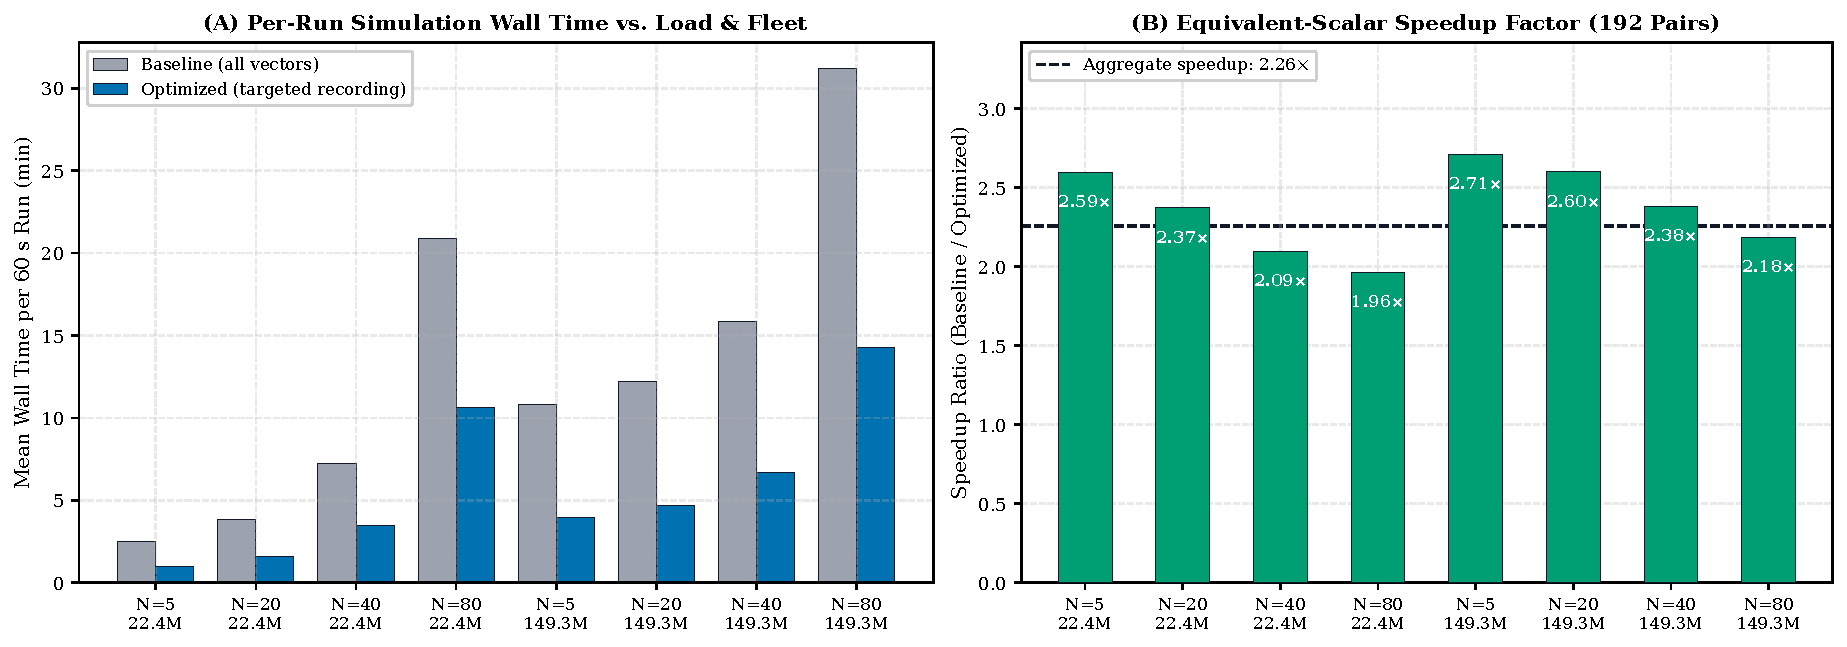
\includegraphics[width=0.92\textwidth]{images/pdf/fig_runtime_speedup.pdf}
\caption{Simulator runtime-optimization benchmark across $192$ paired baseline configurations ($384$ runs total): (A)~mean wall-clock duration per \qty{60}{\second} run versus fleet size and telemetry load; (B)~per-condition speedup factor ($2.26\times$ aggregate speedup across \qty{41.76}{core\text{-}hours} $\to$ \qty{18.50}{core\text{-}hours}).}
\label{fig:speedup}
\end{figure}

\FloatBarrier
\section{Dataset Accounting, Traceability, and Artifact Inventory}
\label{app:traceability}

\Cref{tab:pool_decomposition} summarizes the exact set decomposition and overlap arithmetic across the three analytical pools and the \num{6947}-run archive, \Cref{tab:req_coverage} maps the core architectural and analytical specifications to their validation locations in this report, and the artifact inventory documents the frozen campaign snapshot anchored at commit \texttt{8730cbe} and the validation package anchored at commit \texttt{3655aa3} (with INET commit \path{dfe270b21f}).

\begin{table}[!tb]
\centering
\footnotesize
\caption{Set decomposition and overlap arithmetic of the \num{6947}-run $80$-point validation archive (full factorial coverage at $R \ge 3$).}
\label{tab:pool_decomposition}
\begin{tabularx}{\textwidth}{l r r l Y}
\toprule
\textbf{Dataset Subset / Pool} & \textbf{Points} & \textbf{Runs} & \textbf{Seeds $R$} & \textbf{Exact Set Relationship \& Analytical Role} \\
\midrule
1. core-R3 (4-load balanced) & $40$ & $720$ & Uniform $3$ & $\Namr \in \{5, 10, 20, 40, 80\} \times \{22.4, 74.7, 95.0, 149.3\}\,\text{Mbps}$; balanced fleet scaling \\
2. knee-R3 (8-load balanced) & $48$ & $864$ & Uniform $3$ & $\Namr \in \{10,20,40\} \times \text{all } 8\text{ loads}$; wired knee \& LOO PCHIP validation \\
\quad $\hookrightarrow$ Overlap $|\mathrm{core\text{-}R3} \cap \mathrm{knee\text{-}R3}|$ & $24$ & $432$ & Uniform $3$ & $\Namr \in \{10,20,40\} \times 4\text{ base loads}$ shared by both balanced $R=3$ pools \\
\quad $\hookrightarrow$ Remainder at $\Namr \in \{5, 80\}$ & $16$ & $288$ & Uniform $3$ & Interior loads $\{45, 60, 85, 110\}\,\text{Mbps}$ at $\Namr \in \{5, 80\}$ ($\implies \num{1440}$ base $R=3$) \\
3. Extra paired reps in supp-maxR & $49$ & \num{5484} & $R \in \{5,22\}$ & $48$ slices at $R=22$ ($\Namr \in \{10,40,80\}$) + $1$ at $R=5$ ($\Namr=20$, \qty{12}{\mbps}, \qty{22.4}{\mbps}; $\text{rep} \ge 3$) \\
\quad $\hookrightarrow$ \textbf{Total supp-maxR pool} & $\mathbf{80}$ & $\mathbf{6{,}924}$ & $\mathbf{3\text{ to }22}$ & $\num{1440} + \num{5484} = \num{6924}$ paired 6-cell runs (full grid, regime map \& tails) \\
4. Post-hoc Cell~1 collapse seeds & $1$ & $23$ & $r \in [22, 44]$ & Unpaired Cell~1 only at $(80, \qty{12}{\mbps}, \qty{22.4}{\mbps})$, extending $R=22 \to 45$ \\
\midrule
\textbf{Frozen Validation Archive} & $\mathbf{80/80}$ & $\mathbf{6{,}947}$ & $\mathbf{3\text{ to }45}$ & $\num{6924}$ paired + $23$ post-hoc Cell~1 = \num{6947} runs (\num{3106282724} valid packets, $0$ conservation error) \\
\bottomrule
\end{tabularx}
\end{table}

\begin{table}[!tb]
\centering
\footnotesize
\caption{Traceability matrix linking system design and simulator specifications to validation evidence.}
\label{tab:req_coverage}
\begin{tabularx}{\textwidth}{P{2.6cm} P{3.6cm} Y P{2.6cm}}
\toprule
\textbf{Requirement Area} & \textbf{Specification} & \textbf{Validation Evidence} & \textbf{Report Location} \\
\midrule
1. Six-Cell Matrix \& Topology & 3 wired (FIFO, 802.1Q, TAS) $\times$ 2 wireless (CSMA/CA, TDMA); 80-packet switch buffer parity & Evaluated across all $80/80$ operating points (\num{6924} paired runs + \num{23} post-hoc collapse seeds; \num{6947} total runs) plus a 9-run Cell~3 80-packet TC0 buffer-parity control; spatial port orthogonality verified on \texttt{eth[0]} and \texttt{eth[1]}. & \Cref{sec:topology,sec:codesign_pilot}; \Cref{fig:topology}; \Cref{tab:six_cell_matrix,tab:traffic_inputs,tab:bufparity_pilot} \\
\addlinespace[2pt]
2. Four Industrial Traffic Classes & Orders (\qty{600}{\byte}), DDS (\qty{200}{\byte}), State (\qty{1000}{\byte}), Telemetry (\qty{1400}{\byte}) & Evaluated across $D \in \{1, 2, 5, 10, 20, 50, 100\}\,\text{ms}$; full-MTU (\qty{1472}{\byte}) and multi-frame VDA~5050 orders (\qtyrange{2100}{11500}{\byte}) checked against GCL guard bands. & \Cref{sec:analytical_wired,sec:rq1,sec:codesign_pilot}; \Cref{tab:deadline_spectrum,tab:gcl_pilot}; \Cref{fig:vda_gcl} \\
\addlinespace[2pt]
3. Three-Stream RNG Isolation & \texttt{rng-0} MAC, \texttt{rng-1} traffic/phases, \texttt{rng-2} AMR positions & Verified via 192-pair runtime-optimization equivalence audit (\num{688320} scalars, $0$ mismatches), 45-run \texttt{-{}-no-jemalloc} canary, and paired cross-cell seed contrasts. & \Cref{sec:topology,app:speedup}; \Cref{fig:speedup} \\
\addlinespace[2pt]
4. 64-Bit Fixed-Point TDMA & \texttt{simtime\_t::raw()} arithmetic; merged AP slot block & Zero wireless retry drops and zero Orders drops across all \num{3462} \texttt{ScheduledDcf} runs; zero AP grant releases under fixed zero-offset TAS pacing in Cell~6 ($0$ vs.\ $521$ each in Cells~2 and~4). & \Cref{sec:analytical_wireless,sec:micro_diagnostics}; \Cref{tab:tdma_feasibility}; \Cref{fig:timing_diagrams,fig:wireless_diagnostics} \\
\addlinespace[2pt]
5. Domain Delay \& Conservation & 3-domain timestamps ($g, t_{\mathrm{ap}}, t_{\mathrm{sw}}, a$) and five-outcome packet ledger & Zero integer error across \num{3106282724} valid packets (\num{27788} series); 240-pair naive linear-share baseline evaluated (\num{0}/240 wired exceedances). & \Cref{sec:ner_semantics,sec:rq2}; \Cref{tab:domain_delay_decomp,tab:hypothesis_test} \\
\addlinespace[2pt]
6. NER Semantics \& ZOH / KILL & Tick grid $c = \phi_T + \lceil(g-\phi_T+L_c)/T\rceil T$ at $T \in \{10,50,500\}\,\text{ms}$ & Multi-rate sensitivity, continuous $\MissA$ vs.\ counterfactual $\MissB$ on KILL classes, and delivered State ZOH staleness ($\le \qty{5}{\tick}$ TDMA vs.\ up to \num{1913} ticks CSMA) quantified. & \Cref{sec:ner_semantics,sec:ner_multirate}; \Cref{fig:ner_timeline,fig:ner_interface}; \Cref{tab:ner_multirate} \\
\addlinespace[2pt]
7. Wasserstein PCHIP Lookup & 25-quantile ECDF tables + monotone 1D Wasserstein PCHIP & LOO cross-validation across fleet and load axes (\qtyrange{70.0}{71.1}{\percent} $\Wone$ MAE reduction on \texttt{eth[0]} classes). & \Cref{sec:pchip_accuracy}; \Cref{tab:pchip_loo,tab:pchip_axes}; \Cref{fig:ner_interface}C and D \\
\bottomrule
\end{tabularx}
\end{table}

\paragraph{Artifact Inventory.}
The frozen simulation snapshot is anchored to commit \texttt{8730cbe} and INET commit \path{dfe270b21f}, while the validation package in \path{report/Project Validation/} is anchored to commit \texttt{3655aa3} (five-outcome integer packet conservation passed on all \num{6947}/\num{6947} runs in \path{tool/sync_validation_tables.py}, supplemented by independent-parser corner-plus-10\%-sample scalar and domain-delay audits in \path{analysis/audit_campaign.py} passing on $202/202$ sampled \texttt{core-R3}, $216/216$ sampled \texttt{knee-R3}, and \num{1233}/\num{1233} sampled \texttt{supp-maxR} runs with zero failures, plus the standalone PASTA ingress-serialization test \path{tool/verify_pasta_ingress.py}). All normalized pool exports (\path{tables/{core_r3,knee_r3,supp_maxr}/}) and derived summary tables (\path{tables/extra/}, with per-run cache \path{run_metrics_full.csv} regenerated locally by \path{tool/sync_validation_tables.py}) are built directly from the pool manifests (\path{tables/*_manifest.csv}). Isolated verification pilots for downlink TDMA (\path{pilot_codesign/}), port-specific \texttt{eth[0]} GCL rebalancing (\path{pilot_gcl/}), and Cell~3 80-packet TC0 buffer-parity control (\path{pilot_bufparity/}) accompany \path{tool/sync_validation_tables.py} and the reproducible vector figure generator \path{tool/generate_validation_figures.py} (\path{images/pdf/}).

\FloatBarrier

\printbibliography

\end{document}
